\documentclass[journal,12pt,twocolumn]{IEEEtran}
%
\usepackage{setspace}
\usepackage{gensymb}
%\doublespacing
\singlespacing

%\usepackage{graphicx}
%\usepackage{amssymb}
%\usepackage{relsize}
\usepackage[cmex10]{amsmath}
\usepackage{siunitx}
%\usepackage{amsthm}
%\interdisplaylinepenalty=2500
%\savesymbol{iint}
%\usepackage{txfonts}
%\restoresymbol{TXF}{iint}
%\usepackage{wasysym}
\usepackage{amsthm}
\usepackage{iithtlc}
\usepackage{mathrsfs}
\usepackage{txfonts}
\usepackage{stfloats}
\usepackage{steinmetz}
%\usepackage{bm}
\usepackage{cite}
\usepackage{cases}
\usepackage{subfig}
%\usepackage{xtab}
\usepackage{longtable}
\usepackage{multirow}
%\usepackage{algorithm}
%\usepackage{algpseudocode}
\usepackage{enumitem}
\usepackage{mathtools}
\usepackage{tikz}
\usepackage{circuitikz}
\usepackage{verbatim}
\usepackage{tfrupee}
\usepackage[breaklinks=true]{hyperref}
%\usepackage{stmaryrd}
\usepackage{tkz-euclide} % loads  TikZ and tkz-base
%\usetkzobj{all}
\usetikzlibrary{calc,math}
\usetikzlibrary{fadings}
\usepackage{listings}
    \usepackage{color}                                            %%
    \usepackage{array}                                            %%
    \usepackage{longtable}                                        %%
    \usepackage{calc}                                             %%
    \usepackage{multirow}                                         %%
    \usepackage{hhline}                                           %%
    \usepackage{ifthen}                                           %%
  %optionally (for landscape tables embedded in another document): %%
    \usepackage{lscape}     
\usepackage{multicol}
\usepackage{chngcntr}
%\usepackage{enumerate}

%\usepackage{wasysym}
%\newcounter{MYtempeqncnt}
\DeclareMathOperator*{\Res}{Res}
%\renewcommand{\baselinestretch}{2}
\renewcommand\thesection{\arabic{section}}
\renewcommand\thesubsection{\thesection.\arabic{subsection}}
\renewcommand\thesubsubsection{\thesubsection.\arabic{subsubsection}}

\renewcommand\thesectiondis{\arabic{section}}
\renewcommand\thesubsectiondis{\thesectiondis.\arabic{subsection}}
\renewcommand\thesubsubsectiondis{\thesubsectiondis.\arabic{subsubsection}}

% correct bad hyphenation here
\hyphenation{op-tical net-works semi-conduc-tor}
\def\inputGnumericTable{}                                 %%

\lstset{
%language=C,
frame=single, 
breaklines=true,
columns=fullflexible
}
%\lstset{
%language=tex,
%frame=single, 
%breaklines=true
%}

\begin{document}
%


\newtheorem{theorem}{Theorem}[section]
\newtheorem{problem}{Problem}
\newtheorem{proposition}{Proposition}[section]
\newtheorem{lemma}{Lemma}[section]
\newtheorem{corollary}[theorem]{Corollary}
\newtheorem{example}{Example}[section]
\newtheorem{definition}[problem]{Definition}
%\newtheorem{thm}{Theorem}[section] 
%\newtheorem{defn}[thm]{Definition}
%\newtheorem{algorithm}{Algorithm}[section]
%\newtheorem{cor}{Corollary}
\newcommand{\BEQA}{\begin{eqnarray}}
\newcommand{\EEQA}{\end{eqnarray}}
\newcommand{\define}{\stackrel{\triangle}{=}}

\bibliographystyle{IEEEtran}
%\bibliographystyle{ieeetr}


\providecommand{\mbf}{\mathbf}
\providecommand{\pr}[1]{\ensuremath{\Pr\left(#1\right)}}
\providecommand{\qfunc}[1]{\ensuremath{Q\left(#1\right)}}
\providecommand{\sbrak}[1]{\ensuremath{{}\left[#1\right]}}
\providecommand{\lsbrak}[1]{\ensuremath{{}\left[#1\right.}}
\providecommand{\rsbrak}[1]{\ensuremath{{}\left.#1\right]}}
\providecommand{\brak}[1]{\ensuremath{\left(#1\right)}}
\providecommand{\lbrak}[1]{\ensuremath{\left(#1\right.}}
\providecommand{\rbrak}[1]{\ensuremath{\left.#1\right)}}
\providecommand{\cbrak}[1]{\ensuremath{\left\{#1\right\}}}
\providecommand{\lcbrak}[1]{\ensuremath{\left\{#1\right.}}
\providecommand{\rcbrak}[1]{\ensuremath{\left.#1\right\}}}
\theoremstyle{remark}
\newtheorem{rem}{Remark}
\newcommand{\sgn}{\mathop{\mathrm{sgn}}}
\providecommand{\abs}[1]{\left\vert#1\right\vert}
\providecommand{\res}[1]{\Res\displaylimits_{#1}} 
\providecommand{\norm}[1]{\left\lVert#1\right\rVert}
%\providecommand{\norm}[1]{\lVert#1\rVert}
\providecommand{\mtx}[1]{\mathbf{#1}}
\providecommand{\mean}[1]{E\left[ #1 \right]}
\providecommand{\fourier}{\overset{\mathcal{F}}{ \rightleftharpoons}}
%\providecommand{\hilbert}{\overset{\mathcal{H}}{ \rightleftharpoons}}
\providecommand{\system}{\overset{\mathcal{H}}{ \longleftrightarrow}}
	%\newcommand{\solution}[2]{\textbf{Solution:}{#1}}
\newcommand{\solution}{\noindent \textbf{Solution: }}
\newcommand{\cosec}{\,\text{cosec}\,}
\providecommand{\dec}[2]{\ensuremath{\overset{#1}{\underset{#2}{\gtrless}}}}
\newcommand{\myvec}[1]{\ensuremath{\begin{pmatrix}#1\end{pmatrix}}}
\newcommand{\mydet}[1]{\ensuremath{\begin{vmatrix}#1\end{vmatrix}}}
%\numberwithin{equation}{section}
\numberwithin{equation}{subsection}
%\numberwithin{problem}{section}
%\numberwithin{definition}{section}
\makeatletter
\@addtoreset{figure}{problem}
\makeatother

\let\StandardTheFigure\thefigure
\let\vec\mathbf
%\renewcommand{\thefigure}{\theproblem.\arabic{figure}}
\renewcommand{\thefigure}{\theproblem}
%\setlist[enumerate,1]{before=\renewcommand\theequation{\theenumi.\arabic{equation}}
%\counterwithin{equation}{enumi}


%\renewcommand{\theequation}{\arabic{subsection}.\arabic{equation}}

\def\putbox#1#2#3{\makebox[0in][l]{\makebox[#1][l]{}\raisebox{\baselineskip}[0in][0in]{\raisebox{#2}[0in][0in]{#3}}}}
     \def\rightbox#1{\makebox[0in][r]{#1}}
     \def\centbox#1{\makebox[0in]{#1}}
     \def\topbox#1{\raisebox{-\baselineskip}[0in][0in]{#1}}
     \def\midbox#1{\raisebox{-0.5\baselineskip}[0in][0in]{#1}}

\vspace{3cm}

\title{
	\logo{
Solutions to Plane Coordinate Geometry by S L Loney
	}
}
\author{ G V V Sharma$^{*}$% <-this % stops a space
	\thanks{*The author is with the Department
		of Electrical Engineering, Indian Institute of Technology, Hyderabad
		502285 India e-mail:  gadepall@iith.ac.in. All content in this manual is released under GNU GPL.  Free and open source.}
	
}	
%\title{
%	\logo{Matrix Analysis through Octave}{\begin{center}\includegraphics[scale=.24]{tlc}\end{center}}{}{HAMDSP}
%}


% paper title
% can use linebreaks \\ within to get better formatting as desired
%\title{Matrix Analysis through Octave}
%
%
% author names and IEEE memberships
% note positions of commas and nonbreaking spaces ( ~ ) LaTeX will not break
% a structure at a ~ so this keeps an author's name from being broken across
% two lines.
% use \thanks{} to gain access to the first footnote area
% a separate \thanks must be used for each paragraph as LaTeX2e's \thanks
% was not built to handle multiple paragraphs
%

%\author{<-this % stops a space
%\thanks{}}
%}
% note the % following the last \IEEEmembership and also \thanks - 
% these prevent an unwanted space from occurring between the last author name
% and the end of the author line. i.e., if you had this:
% 
% \author{....lastname \thanks{...} \thanks{...} }
%                     ^------------^------------^----Do not want these spaces!
%
% a space would be appended to the last name and could cause every name on that
% line to be shifted left slightly. This is one of those "LaTeX things". For
% instance, "\textbf{A} \textbf{B}" will typeset as "A B" not "AB". To get
% "AB" then you have to do: "\textbf{A}\textbf{B}"
% \thanks is no different in this regard, so shield the last } of each \thanks
% that ends a line with a % and do not let a space in before the next \thanks.
% Spaces after \IEEEmembership other than the last one are OK (and needed) as
% you are supposed to have spaces between the names. For what it is worth,
% this is a minor point as most people would not even notice if the said evil
% space somehow managed to creep in.



% The paper headers
%\markboth{Journal of \LaTeX\ Class Files,~Vol.~6, No.~1, January~2007}%
%{Shell \MakeLowercase{\textit{et al.}}: Bare Demo of IEEEtran.cls for Journals}
% The only time the second header will appear is for the odd numbered pages
% after the title page when using the twoside option.
% 
% *** Note that you probably will NOT want to include the author's ***
% *** name in the headers of peer review papers.                   ***
% You can use \ifCLASSOPTIONpeerreview for conditional compilation here if
% you desire.




% If you want to put a publisher's ID mark on the page you can do it like
% this:
%\IEEEpubid{0000--0000/00\$00.00~\copyright~2007 IEEE}
% Remember, if you use this you must call \IEEEpubidadjcol in the second
% column for its text to clear the IEEEpubid mark.



% make the title area
\maketitle

\newpage

\tableofcontents

\bigskip

\renewcommand{\thefigure}{\theenumi}
\renewcommand{\thetable}{\theenumi}
%\renewcommand{\theequation}{\theenumi}

%\begin{abstract}
%%\boldmath
%In this letter, an algorithm for evaluating the exact analytical bit error rate  (BER)  for the piecewise linear (PL) combiner for  multiple relays is presented. Previous results were available only for upto three relays. The algorithm is unique in the sense that  the actual mathematical expressions, that are prohibitively large, need not be explicitly obtained. The diversity gain due to multiple relays is shown through plots of the analytical BER, well supported by simulations. 
%
%\end{abstract}
% IEEEtran.cls defaults to using nonbold math in the Abstract.
% This preserves the distinction between vectors and scalars. However,
% if the journal you are submitting to favors bold math in the abstract,
% then you can use LaTeX's standard command \boldmath at the very start
% of the abstract to achieve this. Many IEEE journals frown on math
% in the abstract anyway.

% Note that keywords are not normally used for peerreview papers.
%\begin{IEEEkeywords}
%Cooperative diversity, decode and forward, piecewise linear
%\end{IEEEkeywords}



% For peer review papers, you can put extra information on the cover
% page as needed:
% \ifCLASSOPTIONpeerreview
% \begin{center} \bfseries EDICS Category: 3-BBND \end{center}
% \fi
%
% For peerreview papers, this IEEEtran command inserts a page break and
% creates the second title. It will be ignored for other modes.
%\IEEEpeerreviewmaketitle

\begin{abstract}
This book provides a vector approach to analytical geometry.  The content and exercises are based on  S L Loney's book on 
Plane Coordinate Geometry.
\end{abstract}

\section{ Coordinates}
\subsection{1 }
\renewcommand{\theequation}{\theenumi}
\renewcommand{\thefigure}{\theenumi}
\begin{enumerate}[label=\thesubsection.\arabic*.,ref=\thesubsection.\theenumi]
\numberwithin{equation}{enumi}
\numberwithin{figure}{enumi}

\item Find the distance between the following pair of points (2,3) and (5,7). 
\\
\solution
%\input{solutions/1/1/Assignment_2.tex}

\item Find the coordinates of the point which divides, internally and externally, the line joining (-3,-4) to (-8,7) in the ratio 7:5
\\
\solution

Let
\begin{align}
    \Vec{A}=\myvec{-3\\-4}
\end{align}
\begin{align}
    \Vec{B}=\myvec{-8\\7}
\end{align}
\begin{enumerate}
\item Using section formula for internal division, 
\begin{align}
\vec{S}&=\large{\frac{7\myvec{-8\\7}+5\myvec{-3\\-4}}{\brak{7+5}}}   
\\
&=\frac{1}{12}\myvec{{-71} \\ {29}}
\end{align}
\item Similarly, for external division, 
\begin{align}
\vec{S}&=\large{\frac{7\myvec{-8\\7}-5\myvec{-3\\-4}}{\brak{7-5}}}   
&=\frac{1}{2} \myvec{{-41} \\ {69}}
\end{align}

Fig. \ref{1/18fig} plots the desired points.
\begin{figure}[!ht]
\centering
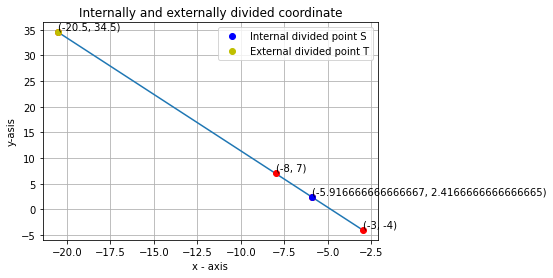
\includegraphics[width=\columnwidth]{solutions/1/18/Internal and external point.png}
\caption{ Plot of coordinate of the point which divides internally and externally }
\label{1/18fig}
\end{figure}
 \end{enumerate} 
 
%
\item The line joining the points (1, -2) and (-3,4) is  trisected;Find the coordinates of the points of the trisection.
\\
\solution
Let 
%
\begin{align}
    \Vec{A}=\myvec{1\\-2},
    \Vec{B}=\myvec{-3\\4}
\end{align}
%
Then, 
\begin{align}
\vec{Q}&=\frac{2\myvec{-3\\4}+1\myvec{1\\-2}}{\brak{1+2}}   \\
&
=\myvec{\frac{-5}{3}\\[0.2cm]{2}}
\\
\vec{P}&=\frac{1\myvec{-5/3\\2}+1\myvec{1\\-2}}{\brak{1+1}}   
\\
&=\myvec{\frac{-1}{3} \\[0.2cm]{0}}
\end{align}
Fig. \ref{1/19/python fig1.png} verifies the result.
\begin{figure}[!ht]
\centering
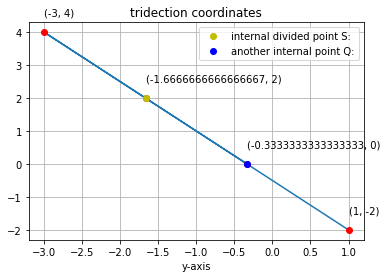
\includegraphics[width=\columnwidth]{solutions/1/19/assignment.1.pythom plot.png}
\caption{ Plot of coordinates}
\label{1/19/python fig1.png}
\end{figure}


 



% \item The coordinates of the vertices of a triangle are $(x_1,y_1)$, $(x_2,y_2)$ and $(x_3,y_3)$. The line joining the first two is divided in the ratio $l:k$, and the line joining his point of division to the opposite angular point is then divided in the ratio  $m:k+l$. Find the coordinates of the latter point of section. 
% %
% \\
% \solution
% From elementary analysis of coordinate geometry and in view of Fig.\ref{eq:solutions/2/22/f2}, as $\bf{D}$ divides the line AB in the ratio $AD:DC=l:k$, we have:

\begin{equation}
 {\bf{D}}=\frac{l{\bf{B}}+k\bf{A}}{l+k}
    \label{eq:solutions/2/22/eq4}
\end{equation}
The position vector $\bf{E}$ which  divides CD in the ratio $DE:EC=m:l+k$,  is clearly obtained by setting $l=m,k=l+k,\bf{A=D,B=C}$ and is given by: 

\begin{equation}
 {\bf{E}}=\frac{m{\bf{C}}+(l+k)\bf{D}}{m+l+k}
    \label{eq:solutions/2/22/eq5}
\end{equation}
 
Using Eq.\ref{eq:solutions/2/22/eq4} into Eq.\ref{eq:solutions/2/22/eq5} and simplifying yields :
\begin{equation}
 {\bf{E}}=\frac{m {\bf{C}}+l{\bf{B}}+k{\bf{A}}}{m+l+k}
    \label{eq:solutions/2/22/eq6}
\end{equation}

Where,
%\begin{align}
 $  \bf{A}  = \begin{pmatrix}
           x_{1} \\
           y_{1} \\
         \end{pmatrix}$, $ \bf{B}  = \begin{pmatrix}
           x_{2} \\
           y_{2} \\
         \end{pmatrix}$  and $  \bf{C}  = \begin{pmatrix}
           x_{3} \\
           y_{3} \\
         \end{pmatrix}$
         
In Fig.\ref{eq:solutions/2/22/f2}, the solution obtained from the Python code is depicted for a particular choice of input viz. $l=1,m=1,k=1$ and $A(0,0),B(3,3)\, $\&$\, C(6,0)$.
Using, Eq.\ref{eq:solutions/2/22/eq6} and the above mentioned input, we have:

$  \bf{E}  = \begin{pmatrix}
           x_{E} \\
           y_{E} \\
         \end{pmatrix}$ $=\begin{pmatrix}
           3 \\
           1 \\
         \end{pmatrix}$



 \begin{figure}[!ht]
    \centering
    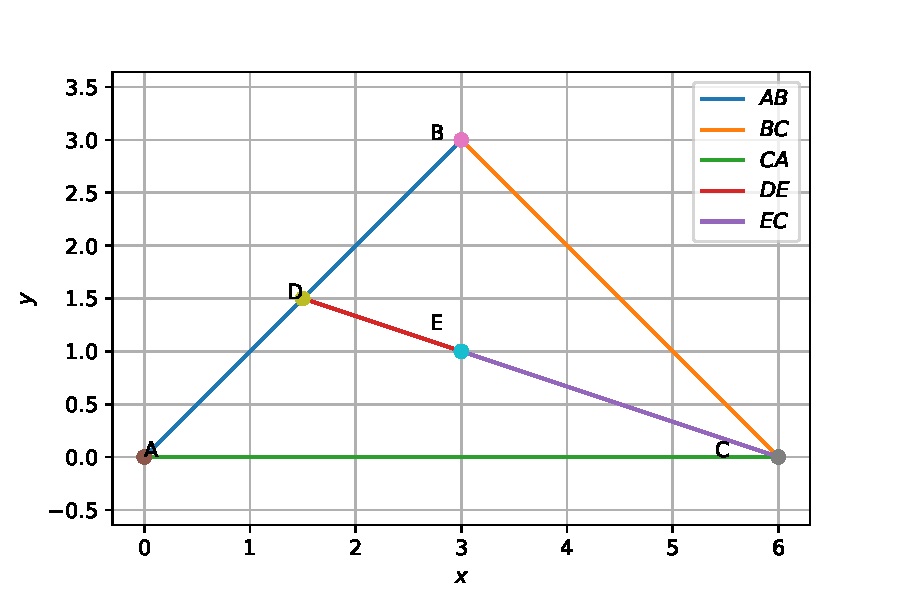
\includegraphics[width=\columnwidth]{./solutions/2/22/Ex1prob22.pdf}
    \caption{For $l=1,m=1,k=1$ and $A(0,0),B(3,3)\, $\&$\, C(6,0)$, the solution $E(3,1)$ is obtained using Python}
    \label{eq:solutions/2/22/f2}
\end{figure}
       


\end{enumerate}

\section{ The Straight Line}
\subsection{6}
\renewcommand{\theequation}{\theenumi}
\renewcommand{\thefigure}{\theenumi}
\begin{enumerate}[label=\thesubsection.\arabic*.,ref=\thesubsection.\theenumi]
\numberwithin{equation}{enumi}
\numberwithin{figure}{enumi}
%
\item Find the equation to the straight line passing through $(2,3)$ and perpendicular to the straight line: $4x-3y=10$.
%
\\
\solution
The vector which is normal to $4x-3y=10$ from simple inspection is :$\myvec{4\\-3}$. Clearly, the  direction vector $\bf{m}$ of a line which is perpendicular to the given line is :

\begin{equation}
\bf{m}=\myvec{3\\-4}
\label{eq:solutions/6/8/eq10}
\end{equation}
The equation of this line which is perpendicular to the given line and  passing through $\bf{A}=\myvec{x_A\\y_A}$ is then obtained as:
\begin{equation}
  {\bf{m^Tx}}=\bf{m^TA}
    \label{eq:solutions/6/8/eq20}
\end{equation}
\eqref{eq:solutions/6/8/eq20} simplifies to read:

\begin{equation}
 \myvec{3 &4 \\}\bf{x}=18 
    \label{eq:solutions/6/8/eq30}
\end{equation}
Which in scalar form reads: $3x+4y=18$
        
Both the straight lines are plotted in Fig. \ref{eq:solutions/6/8/ExVIprob8.pdf} along with the point $A(2,3)$ using Python script.      
        
\begin{figure}[ht]
    \centering
    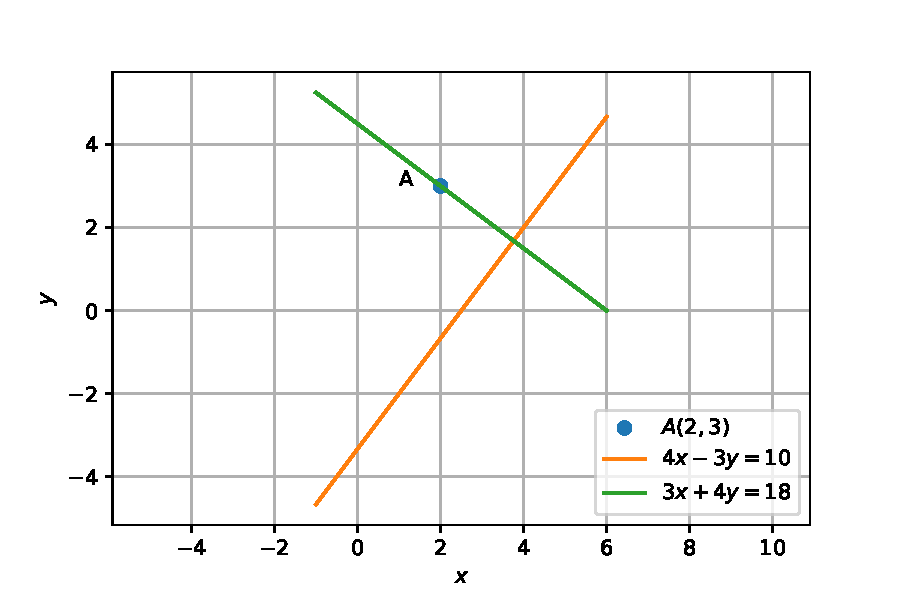
\includegraphics[width=\columnwidth]{./solutions/6/8/ExVIprob8.pdf}
    \caption{Solution}
    \label{eq:solutions/6/8/ExVIprob8.pdf}
\end{figure}




\end{enumerate}

\section{ The Circle}
\subsection{17}
\renewcommand{\theequation}{\theenumi}
\renewcommand{\thefigure}{\theenumi}
\begin{enumerate}[label=\thesubsection.\arabic*.,ref=\thesubsection.\theenumi]
\numberwithin{equation}{enumi}
\numberwithin{figure}{enumi}

\item Find the equation to the circle which passes through the points $\myvec{ 1 \\ -2 }$ and $\myvec{ 4 \\ -3 }$ and which has its centre on the straight line $\myvec{ 3 & 4 }x = 7$.
%
\\
\solution
The equation of circle can be expressed as
\begin{align}
    \vec{x}^T\vec{x}-2\vec{C}^T\vec{x}+f = 0
\end{align}
$\vec{C}$ is the centre  and substituting the points in the equation of circle we get
\begin{align}
2\myvec{1 & -2}\vec{C}-f &= 5\\
2\myvec{4 & -3}\vec{C}-f &= 25\\
\myvec{3 & 4}\vec{C} &= 7
\end{align}
can be expressed in matrix form
\begin{align}
\myvec{3 & 4 & 0 \\
2 & -4 & -1 \\
8 & -6 & -1}
\myvec{\vec{C}\\f} = \myvec{ 7 \\ 5 \\ 25}
\end{align}

Row reducing the augmented matrix
\begin{align}
\myvec{3 & 4 & 0 & 7\\
2 & -4 & -1 & 5 \\
8 & -6 & -1 & 25}
\xleftrightarrow{R_1\leftarrow R_1/3}
\myvec{1 & \frac{4}{3} & 0 & \frac{7}{3}\\ \\
2 & -4 & -1 & 5 \\ 
8 & -6 & -1 & 25}
\end{align}

\begin{align}
\xleftrightarrow[R_3\leftarrow R_3 - 8R_1]{R_2\leftarrow R_2 - 2R_1}
\myvec{1 & \frac{4}{3} & 0 & \frac{7}{3}\\ \\
0 & \frac{-20}{3} & -1 & \frac{1}{3} \\ \\
0 & \frac{-50}{3} & -1 & \frac{19}{3}}
\end{align}

\begin{align}
\xleftrightarrow{R_2\leftarrow \frac{-3}{20}R_2 }
\myvec{1 & \frac{4}{3} & 0 & \frac{7}{3}\\ \\
0 & 1 & \frac{3}{20} & \frac{-1}{20} \\ \\
0 & \frac{-50}{3} & -1 & \frac{19}{3}}
\end{align}

\begin{align}
\xleftrightarrow{R_3\leftarrow R_3 + \frac{50}{3}R_2}
\myvec{1 & \frac{4}{3} & 0 & \frac{7}{3}\\ \\
0 & 1 & \frac{3}{20} & \frac{-1}{20} \\ \\
0 & 0 & \frac{3}{2} & \frac{11}{2}}
\end{align}
\begin{align}
\vec{C} = \myvec{\frac{47}{15}  \\ \\ \frac{-3}{5} }
f = \frac{11}{3}
\end{align}
\begin{align}
f = \frac{11}{3}
\end{align}
The required circle equation,
\begin{align}
\vec{x}^T\vec{x}-2\myvec{\frac{47}{15} & \frac{-3}{5} }\vec{x} + \frac{11}{3} = 0
\end{align}

\begin{figure}[!ht]
\centering
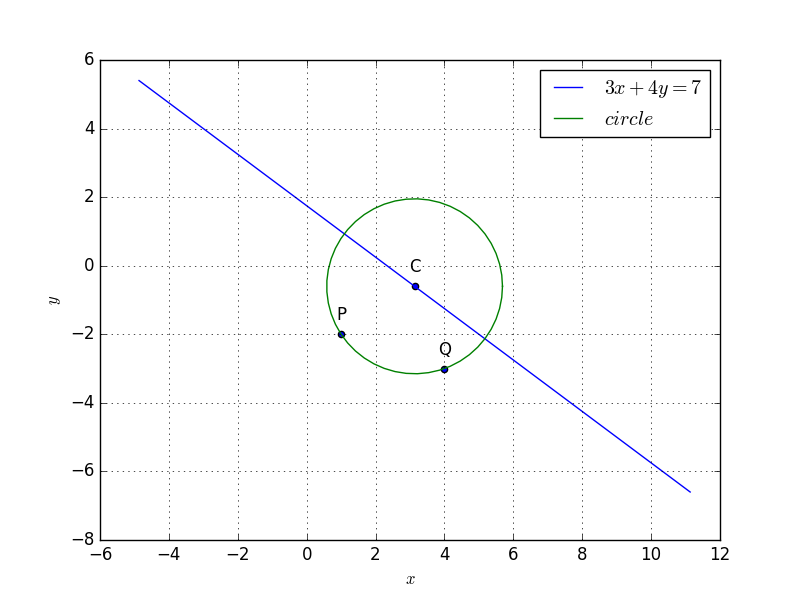
\includegraphics[width=\columnwidth]{./solutions/17/13/figure.png}
\caption{Circle passing through point P and Q also centre lie on the line 3x+4y=7}
\label{eq:solutions/17/13/Fig}
\end{figure}

Find the equation to the circle that passes through the points:
\begin{align}
\vec{x_1} = \myvec{1\\2},\vec{x_2} = \myvec{3\\-4} , \vec{x_3} = \myvec{5\\-6}
\end{align}
\solution
The equation of circle in vector form is given by:
\begin{align}
\vec{x^Tx}+2\vec{x^Tu}+f = 0 \label{eq:solutions/17/16/eq:1}
\end{align}
Using $\vec{x_1}, \vec{x_2}, \vec{x_3}$ in \eqref{eq:solutions/17/16/eq:1},
\begin{align}
\vec{x_1}^T\vec{x_1}+2\vec{x_1}^T\vec{u}+f=0\\
\vec{x_2}^T\vec{x_2}+2\vec{x_2}^T\vec{u}+f=0\\
\vec{x_3}^T\vec{x_3}+2\vec{x_3}^T\vec{u}+f=0
\end{align}
The above system can be written in matrix form as:
\begin{align}
\myvec{2\vec{x_1}^T & 1\\2\vec{x_2}^T & 1\\2\vec{x_3}^T & 1}\myvec{\vec{u}\\f}=\myvec{-\vec{x_1}^T\vec{x_1}\\-\vec{x_1}^T\vec{x_1}\\-\vec{x_3}^T\vec{x_3}} \label{eq:solutions/17/16/eq:2}
\end{align}
Substituting the values for $\vec{x_1}, \vec{x_2}, \vec{x_3}$ in \eqref{eq:solutions/17/16/eq:2},
\begin{align}
\myvec{2 & 4 & 1\\6 & -8 & 1\\10 & -12 & 1}\myvec{\vec{u}\\f}&=\myvec{-5\\-25\\-61} \label{eq:solutions/17/16/eq:3}
\end{align}
Using row echelon form to reduce \eqref{eq:solutions/17/16/eq:3}, we get:
\begin{align}
\xleftrightarrow[R_3\rightarrow R_3-5R_1]{R_2\rightarrow R_2-3R_1}\myvec{2 & 4 & 1 & -5\\0 & -20 & -2 & -10\\ 0 & -32 & -4 & -36}\\
\xleftrightarrow[R_3\rightarrow -\frac{1}{4}R_3]{R_2 \rightarrow -\frac{1}{2}R_2}\myvec{2 & 4 & 1 & -5\\0 & 10 & 1 & 5\\ 0 & 8 & 1 & 9}\\
\xleftrightarrow[]{R_3 \rightarrow 5R_3-4R_2}\myvec{2 & 4 & 1 & -5\\0 & 10 & 1 & 5\\ 0 & 0 & 1 & 25}\\ \label{eq:solutions/17/16/eq:4}
\xleftrightarrow[R_2 \rightarrow \frac{1}{10}R_2]{R_1 \rightarrow \frac{1}{2}R_1}\myvec{1 & 2 & \frac{1}{2} & -\frac{5}{2}\\[0.2cm]0 & 1 & \frac{1}{10} & \frac{2}{5}\\[0.2cm] 0 & 0 & 1 & 25}
\end{align}
Back solving the system using \eqref{eq:solutions/17/16/eq:2} and \eqref{eq:solutions/17/16/eq:4}, we get:
\begin{align}
\myvec{\vec{u}\\f}=\myvec{-11 \\ -2 \\ 25} \\
\implies \vec{u} = \myvec{-11 \\ -2}, f = 25
\end{align}
The equation of the circle that passes through the points $\vec{x_1}, \vec{x_2}, \vec{x_3}$ is given by:
\begin{align}
\vec{x^Tx}+2\myvec{-11 \\ -2}^T\vec{x}+f = 0 \\
\implies x^2 + y^2 - 22x -4y + 25 = 0
\end{align}
The plot of the circle is given below:
\begin{figure}[t]
\centering
    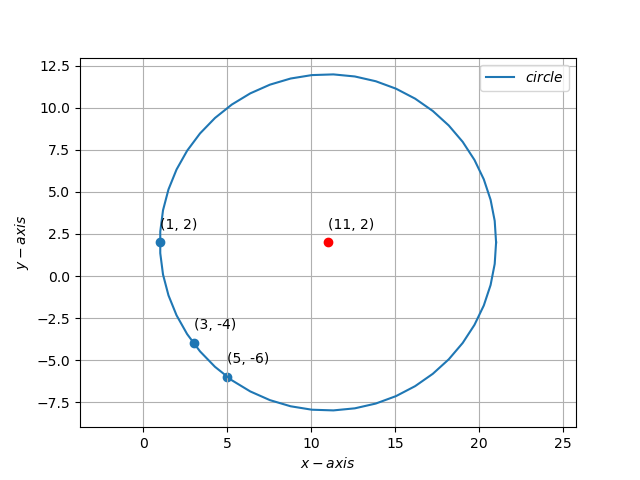
\includegraphics[width=\columnwidth]{solutions/17/16/Latex/Figure_1.png}
    \caption{Circle centered at $(11, 2)$ with radius $10$.}
    \label{eq:solutions/17/16/fig:1}
\end{figure}


\item Find the equation of circle passing through the points
\begin{align}
    \vec{x_1}=\myvec{1\\1}, \vec{x_2}=\myvec{2\\-1}, \vec{x_3}=\myvec{8\\2}\label{eq:solutions/17/17/eq:0}
\end{align}
%
\\
\solution
Vector form of the equation of circle is :
\begin{align}
\vec{x}^T\vec{x}+2\vec{x}^T\vec{u}+f=0\label{eq:solutions/17/17/eq:1}
\end{align}
For $\vec{x_1}$, $\vec{x_2}$ and $\vec{x_3}$ equation \eqref{eq:solutions/17/17/eq:1} can be written as:
\begin{align}
\vec{x_1}^T\vec{x_1}+2\vec{x_1}^T\vec{u}+f=0\\
\vec{x_2}^T\vec{x_2}+2\vec{x_2}^T\vec{u}+f=0\\
\vec{x_3}^T\vec{x_3}+2\vec{x_3}^T\vec{u}+f=0
\end{align}
In matrix form this can be written as :
\begin{align}
    \myvec{2\vec{x_1}^T&1\\2\vec{x_2}^T&1\\2\vec{x_3}^T&1}\myvec{\vec{u}\\f}&=\myvec{-\vec{x_1}^T\vec{x_1}\\-\vec{x_1}^T\vec{x_1}\\-\vec{x_3}^T\vec{x_3}}\label{eq:solutions/17/17/eq:5}
\end{align}
By putting the values of $\vec{x_1},\vec{x_2}$ and $\vec{x_3}$ from \eqref{eq:solutions/17/17/eq:0} in \eqref{eq:solutions/17/17/eq:5} we get :   
\begin{align}
 \myvec{2&2&1\\4&-2&1\\16&4&1}\myvec{\vec{u}\\f}&=\myvec{-2\\-5\\-68} \label{eq:solutions/17/17/eq:6}
\end{align}
Using Gaussian Elimination method :
\begin{align}
\xleftrightarrow[R_2 \leftarrow R_2-4R_1]{R_1 \leftarrow \frac{1}{2}R_1}\myvec{1&1&\frac{1}{2}&-1\\0&-6&-1&-1\\16&4&1&-68}\\
\xleftrightarrow{R_3 \leftarrow R_3-16R_1}\myvec{1&1&\frac{1}{2}&-1\\0&-6&-1&-1\\0&-12&-7&-52}\\
\xleftrightarrow[R_3 \leftarrow R_3+124R_2]{R_2 \leftarrow -\frac{1}{6}R_2}\myvec{1&1&\frac{1}{2}&-1\\[0.2cm]0&1&\frac{1}{6}&\frac{1}{6}\\[0.2cm]0&0&-5&-50}\label{eq:solutions/17/17/eq:9}
\end{align}
Using \eqref{eq:solutions/17/17/eq:6} and \eqref{eq:solutions/17/17/eq:9} we get : 
\begin{align}
\myvec{\vec{u}\\f}&=\myvec{-\frac{9}{2}\\[0.1cm]-\frac{3}{2}\\[0.1cm]10}\\
\vec{u}&=\myvec{-\frac{9}{2}\\[0.1cm]-\frac{3}{2}}\\
f&=10   
\end{align}
By putting the values of $\vec{u}$ and f in \eqref{eq:solutions/17/17/eq:1} we get : 
\begin{align}
\vec{x}^T\vec{x}+2\myvec{-\frac{9}{2}\\[0.1cm]-\frac{3}{2}}^T\vec{x}+10&=0\label{eq:solutions/17/17/eq:14}\\
x^2+y^2-9x-6y+10&=0\label{eq:solutions/17/17/eq:15}
\end{align}
Plot of the circle given by equation \eqref{eq:solutions/17/17/eq:15} is as follows :
\begin{figure}[h]
\centering
    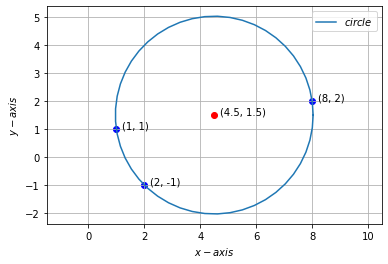
\includegraphics[width=\columnwidth]{solutions/17/17/circle3.png}
    \caption{A circle centered at $(4.5, 1.5)$ with radius $3.53$.}
    \label{eq:solutions/17/17/circle}
\end{figure}


\end{enumerate}

\subsection{18}
\renewcommand{\theequation}{\theenumi}
\renewcommand{\thefigure}{\theenumi}
\begin{enumerate}[label=\thesubsection.\arabic*.,ref=\thesubsection.\theenumi]
\numberwithin{equation}{enumi}
\numberwithin{figure}{enumi}


\item Write down the equation of the tangent to a circle passing through the point $\vec{p}$. 

Equation of the circle and positional vector $\vec{p}$ is given as :
\begin{align}
    x^2+y^2-3x+10y&=15\label{eq:solutions/18/1/eq:0}\\
    \vec{p}&=\myvec{4\\-11}
\end{align}
\solution


General equation of the circle in vector form is :
\begin{align}
\vec{x}^T\vec{x}+2\vec{u}^T\vec{x}+f=0\label{eq:solutions/18/1/eq:1}
\end{align}
In the vector form \eqref{eq:solutions/18/1/eq:0} can be written as :
\begin{align}
\vec{x}^T\vec{x}+2\myvec{\frac{-3}{2}\\[0.1 cm]5}^T\vec{x}-15=0\label{eq:solutions/18/1/eq:2}
\end{align}
By comparing \eqref{eq:solutions/18/1/eq:1} and \eqref{eq:solutions/18/1/eq:2} we get : 
\begin{align}
    \vec{u}=\myvec{-\frac{3}{2}\\[0.1 cm]5},f=-15\label{eq:solutions/18/1/eq:3}
\end{align}
We know that the equation of tangent in the form of normal vector $(\vec{p}+\vec{u})$ and point $\vec{p}$ can be written as:
\begin{align}
    (\vec{p}+\vec{u})^T(\vec{x}-\vec{p})&=0\\
    (\vec{p}+\vec{u})^T\vec{x}-\vec{p}^T\vec{p}-\vec{u}^T\vec{q}&=0\label{eq:solutions/18/1/eq:5}
\end{align}
Using \eqref{eq:solutions/18/1/eq:1}, \eqref{eq:solutions/18/1/eq:5} will become : 
\begin{align}
    (\vec{p}+\vec{u})^T\vec{x}+\vec{u}^T\vec{p}+f&=0\label{eq:solutions/18/1/eq:6}
\end{align}
By putting the values of $\vec{p}$, $\vec{u}$ and $f$ from \eqref{eq:solutions/18/1/eq:3} in \eqref{eq:solutions/18/1/eq:6} we get : 
\begin{align}
    \myvec{\frac{5}{2}&-6}\vec{x}+\myvec{4&-11}\myvec{\frac{-3}{2}\\[0.2cm]5}-15&=0\\
    \myvec{\frac{5}{2}&-6}\vec{x}-76&=0
\end{align}
Hence the equation of the tangent to the circle passing through the point $\vec{p}$ is:
\begin{align}
    \myvec{\frac{5}{2}&-6}\vec{x}&=76\label{eq:solutions/18/1/eq:9}
\end{align}
Plot of the tangent to a circle given by equation \eqref{eq:solutions/18/1/eq:9} is as follows :
\begin{figure}[h]
\centering
    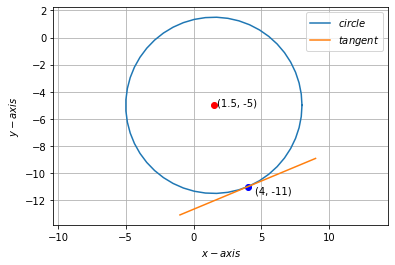
\includegraphics[width=\columnwidth]{solutions/18/1/tangent.png}
    \caption{Tangent to a circle centered at $(1.5, -5)$ with radius $6.5$ passing through the point $(4,-11)$.}
    \label{eq:solutions/18/1/tangent}
\end{figure}


\item Find equation of the tangent to the circle
\begin{align}
  x^2 + y^2 = 4 \label{eq:solutions/18/3/Latex/eq:1}
\end{align}
which is parallel to the line
\begin{align}
  x+2y-6=0  \label{eq:solutions/18/3/Latex/eq:2}
\end{align}
%
\solution
The equations for the circle and line in \eqref{eq:solutions/18/3/Latex/eq:1} and \eqref{eq:solutions/18/3/Latex/eq:2} can be rewritten in vector form as:
\begin{align}
  \norm{\vec{x}}^2 = 4 \\
  \myvec{1 & 2}\vec{x} = 6 \label{eq:solutions/18/3/Latex/eq:3}
\end{align}
The center of the circle happens to be $(0, 0)$ \\
The equation of a line is of the form:
\begin{align}
  \vec{n}^T\vec{x} = c \label{eq:solutions/18/3/Latex/eq:4}
\end{align}
Where n is the normal to the line. \\
Comparing \eqref{eq:solutions/18/3/Latex/eq:4} to \eqref{eq:solutions/18/3/Latex/eq:3},
\begin{align}
  \vec{n} = \myvec{1 \\ 2}
\end{align}
Since the tangent is parallel to the line in \eqref{eq:solutions/18/3/Latex/eq:3}, it will also have the same normal.

The point of contact for a conic is given by:
\begin{align}
  \vec{v} = \vec{V}^{-1}(\kappa\vec{n}-\vec{u}) \label{eq:solutions/18/3/Latex/eq:5}
\end{align}
where,
\begin{align}
  \kappa = \pm \sqrt[]{\frac{\vec{u}^T\vec{V^{-1}u}-f}{\vec{n}^T\vec{V}^{-1}\vec{n}}} \label{eq:solutions/18/3/Latex/eq:6}
\end{align}
For a circle,
\begin{align}
  \vec{V} = \vec{I}
\end{align}
Using properties of identity matrix, we get:
\begin{align}
  \vec{I}^{-1} = \vec{I} \\
  \vec{IX} = \vec{X}
\end{align}
Therefore \eqref{eq:solutions/18/3/Latex/eq:5} and \eqref{eq:solutions/18/3/Latex/eq:6} simplify to:
\begin{align}
  \kappa = \pm \sqrt[]{\frac{\vec{u}^T\vec{u}-f}{\vec{n}^T\vec{n}}} \\
  \implies \vec{v} = \kappa\vec{n-u}
\end{align}
Substituting the values, we get:
\begin{align}
  \kappa = \pm \sqrt[]{\frac{4}{\myvec{1 & 2}\myvec{1 \\ 2}}} \\
  \implies \kappa = \pm \sqrt[]{\frac{4}{5}} \\
  \vec{q} = \pm \sqrt[]{\frac{4}{5}}\myvec{1 \\ 2} \\
  \implies \vec{q_1} = \myvec{\sqrt[]{\frac{4}{5}} \\[0.2cm] \sqrt[]{\frac{16}{5}}}, \vec{q_2} = -\myvec{\sqrt[]{\frac{4}{5}} \\[0.2cm] \sqrt[]{\frac{16}{5}}}
\end{align}
Since there are two points of contact, there are two tangents parallel to \eqref{eq:solutions/18/3/Latex/eq:3} that have the same normal vector.
\begin{align}
  \implies \vec{n}^T\vec{q_1} = c_1 \\
  \vec{n}^T\vec{q_2} = c_2
\end{align}
Substituting the values, we get:
\begin{align}
  c_1 = 2\sqrt[]{5}, c_2 = -2\sqrt[]{5}
\end{align}
Therefore, the equation of the tangents are:
\begin{align}
  \myvec{1 & 2}\vec{x} = 2\sqrt[]{5} \\
  \myvec{1 & 2}\vec{x} = -2\sqrt[]{5}
\end{align}
The plot of the circle with the tangents is given below:
\begin{figure}[h]
\centering
    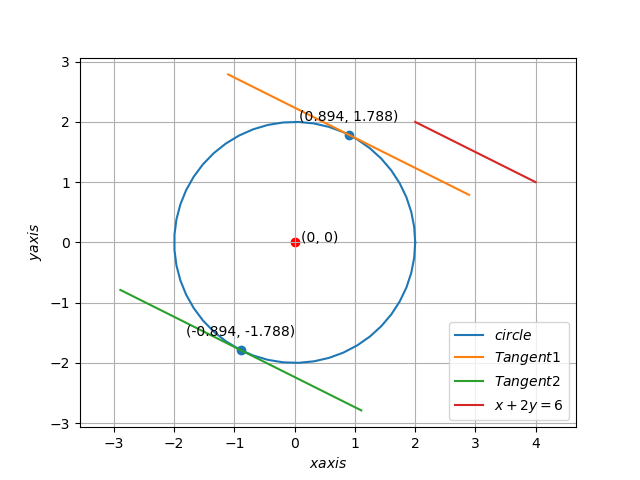
\includegraphics[width=\columnwidth]{solutions/18/3/Latex/Figure_1.png}
    \caption{Circle centered at $(0, 0)$ with tangents parallel to line $x+2y=6$.}
    \label{eq:solutions/18/3/Latex/fig:1}
\end{figure}

\end{enumerate}

\section{Pair of Straight Lines}
\subsection{13}
\renewcommand{\theequation}{\theenumi}
\renewcommand{\thefigure}{\theenumi}
\begin{enumerate}[label=\thesubsection.\arabic*.,ref=\thesubsection.\theenumi]
\numberwithin{equation}{enumi}
\numberwithin{figure}{enumi}
%
\item Prove that the following equations represent two straight lines, find also their point of intersection and the angle between them.\\
$6y^2-xy-x^2+30y+36=0$.
%
\\
\solution

The given equation can be written as:
\begin{align}
-x^2-xy+6y^2+30y+36=0 \label{eq:solutions/13/1/eq1}
\end{align}
\mydet{\vec{V}&\vec{u}\\\vec{u}^T&f} of \eqref{eq:solutions/13/1/eq1} becomes
\begin{align}
    \mydet{-1&-\frac{1}{2}&0\\\frac{-1}{2}&6&15\\0&15&36}=0\label{eq:solutions/13/1/eq02}
\end{align}
Expanding equation \eqref{eq:solutions/13/1/eq02}, we get zero.\\
Hence given equation represents a pair of straight lines.

The general equation second degree is given by
\begin{equation}\label{eq:solutions/13/1/eq5}
	ax^2 + 2bxy + cy^2 + 2dx + 2ey + f = 0
\end{equation}
Let $(\alpha,\beta)$ be their point of intersection, then
\begin{equation}\label{eq:solutions/13/1/eq6}
	\myvec{ a & h\\ h & b}\myvec{\alpha \\ \beta} = \myvec{-d \\ -e}
\end{equation}
Given equation is
\begin{align}
	-x^2-xy+6y^2+30y+36=0
\end{align}
Substituting in \eqref{eq:solutions/13/1/eq6}
\begin{align}
	\label{eq:solutions/13/1/eq16}\myvec{ -1 & \frac{-1}{2}\\\frac{-1}{2} & 6}\myvec{\alpha \\ \beta} = \myvec{0 \\ -15} \\
	\label{eq:solutions/13/1/eq17}\implies \myvec{\alpha \\ \beta} =\myvec{\frac{6}{5} \\ \frac{-12}{5}}
\end{align}
\text{Hence, the intersection point is}
\myvec{\frac{6}{5}\\-\frac{12}{5}}\\
Also, Verified using python code from
\begin{lstlisting}
codes/Assignment_5.py
\end{lstlisting}
From, Spectral decomposition,
\begin{align}
	\vec{V} &= \vec{P}\vec{D}\vec{P}^T\\
	\label{eq:solutions/13/1/eq18}\vec{V} &= \myvec{ -1 & \frac{-1}{2}\\\frac{-1}{2} & 6}\\
	\label{eq:solutions/13/1/eq19}\vec{P} &= \myvec{7-5 \sqrt{2} & 7+5 \sqrt{2}\\ 1 & 1}\\
	\label{eq:solutions/13/1/eq20}\vec{D} &= \myvec{\frac{5+5\sqrt{2}}{2} & 0\\ 0 & \frac{5-5\sqrt{2}}{2}}
\end{align}
P and D are also verified using python code from
\begin{lstlisting}
codes/diagonalize1.py
\end{lstlisting}
Using, \eqref{eq:solutions/13/1/eq17}, \eqref{eq:solutions/13/1/eq19} and \eqref{eq:solutions/13/1/eq20} in,
\begin{align}
	u_1(x-\alpha) + u_2(y-\beta) &= \pm \sqrt{-\frac{\lambda_2}{\lambda_1}}(v_1(x-\alpha) + v_2(y-\beta))\label{eq:solutions/13/1/eq14}
\end{align}
\begin{multline}\label{eq:solutions/13/1/eq21}
\implies	\left(7-5 \sqrt{2}\right)\left(x-\frac{30}{23}\right) + \left(y+\frac{60}{23}\right) \\= \pm \sqrt{-\frac{\frac{5-5\sqrt{2}}{2}}{\frac{5+5\sqrt{2}}{2}}}\left(\left(7-5 \sqrt{2}\right)\left(x-\frac{6}{5}\right) + \left(y+\frac{12}{5}\right)\right)
\end{multline}
simplifying \ref{eq:solutions/13/1/eq21}, we get:
\begin{align}
	\label{eq:solutions/13/1/eq22}-x + 2y + 6 = 0 \text{ and } x + 3y + 6 = 0\\
	\implies (-x + 2y + 6)(x + 3y + 6) = 0\\
	\therefore -x+2y=-6 \quad , \quad x+3y=-6\label{eq:solutions/13/1/eq23}
\end{align}


Angle between two lines, $\theta$ can be given by
\begin{align}
n_1&=(\vec{-2,-1})\\
n_2&=(\vec{-3,1})\\
\cos \theta &= \frac{\vec{n_1}^T\vec{n_2}}{\norm{\vec{n_1}}\norm{\vec{n_2}}}\\
\cos \theta&=\frac{\myvec{-2&-1}\myvec{-3\\1}}{\sqrt{(-2)^2 +(-1)^2} \times \sqrt{+(-3)^2+1}}=\frac{1}{\sqrt{2}}\\
\implies \theta &= 45\degree
\end{align}
\begin{figure}[!h]
\centering
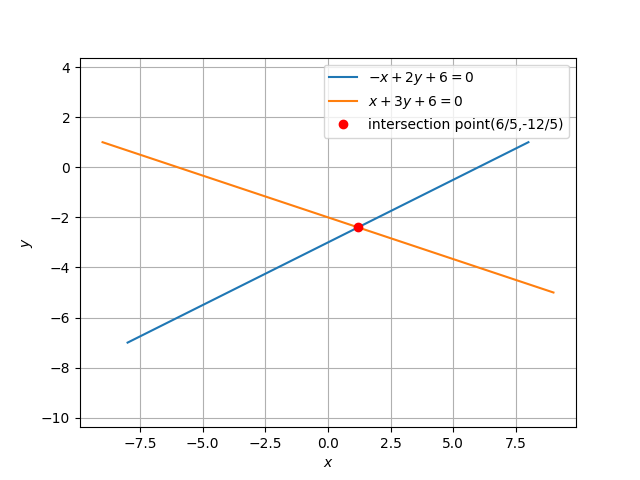
\includegraphics[width=\columnwidth]{./solutions/13/1/Figure_1.png}
\caption{plot showing intersection of lines.}
\label{eq:solutions/13/1/Fig_1}
\end{figure}

\item Prove that the following equations represent two straight lines; and also find their point of intersection and the angle between them
\begin{align}\nonumber
    x^2-5xy+4y^2+x+2y-2=0
\end{align}
\\
\solution
{Proving that given equation represents two straight lines}
The given equation is
\begin{align}\label{eq:solutions/13/2/eq:e1}
    x^2-5xy+4y^2+x+2y-2=0
\end{align}
Comparing this to the standard equation,
\begin{align}
    \vec{V} = \myvec{1 & \frac{-5}{2} \\ \frac{-5}{2} & 4}\\
    \vec{u} = \myvec{\frac{1}{2} \\ 1}\\
    f = -2
\end{align}
\begin{align}\label{eq:solutions/13/2/eq:e3}
    \implies\vec{x}^T\myvec{1 & \frac{-5}{2} \\ \frac{-5}{2} & 4}\vec{x} + 2\myvec{\frac{1}{2} & 1}\vec{x} -2 = 0
\end{align}
Equation \eqref{eq:solutions/13/2/eq:e1} represents a pair of straight lines if
\begin{align}
    \label{eq:solutions/13/2/eq:det}\mydet{\vec{V} & \vec{u}\\ \vec{u}^T & f}=0
\end{align}
\begin{align}
    \delta & = \mydet{1 & \dfrac{-5}{2} & \dfrac{1}{2} \\ \dfrac{-5}{2} & 4 & 1 \\ \dfrac{1}{2} & 1 & -2} \\ & = 0
\end{align}
Hence, proved that given equation represents two straight lines.
{Finding point of intersection between the straight lines}
\begin{align}
    \det V & = \mydet{1 & \frac{-5}{2}\\ \frac{-5}{2} & 4}\\ & = \frac{-9}{4} < 0
\end{align}
Thus, the two straight lines intersect. Let the equation of the straight lines be given as
\begin{align}
    \label{eq:solutions/13/2/eq:line1}\vec{n}_1^T\vec{x}=c_1 \\
    \label{eq:solutions/13/2/eq:line2}\vec{n}_2^T\vec{x}=c_2
\end{align}
with their slopes as $\vec{m}_1$ and $\vec{m}_2$ respectively.

Then the equation of the pair of straight lines is
\begin{align}\label{eq:solutions/13/2/eq:line1line2}
    (\vec{n}_1^T\vec{x}-c_1)(\vec{n}_2^T\vec{x}-c_2) = 0
\end{align}
Using \eqref{eq:solutions/13/2/eq:e3} and \eqref{eq:solutions/13/2/eq:line1line2},
\begin{align}
    (\vec{n}_1^T\vec{x}-c_1)(\vec{n}_2^T\vec{x}-c_2) = \vec{x}^T\myvec{1 & \frac{-5}{2} \\ \frac{-5}{2} & 4}\vec{x} + 2\myvec{\frac{1}{2} & 1}\vec{x} -2
\end{align}
Comparing both sides,
\begin{align}
    c_2\vec{n}_1+c_1\vec{n}_2 = -2\myvec{\frac{1}{2} \\ 1}\label{eq:solutions/13/2/eq:c1c2}\\
    c_1c_2 = -2
\end{align}
Slopes of the lines are roots of the equation
\begin{align}
    cm^2+2bm+a=0 \label{eq:solutions/13/2/eq:slope}\\
    \implies m_i = \frac{-b\pm \sqrt{-\mydet{\vec{V}}}}{c}\\
    \vec{n}_i = k_i\myvec{-m_i \\ 1}
\end{align}
Substituting \eqref{eq:solutions/13/2/eq:e1} in \eqref{eq:solutions/13/2/eq:slope},
\begin{align}
    4m^2-5m+1=0\\
    \implies m_i = \frac{\frac{5}{2}\pm \frac{3}{2}}{4} \\
    \implies m_1 = 1, m_2 = \frac{1}{4}
\end{align}
Therefore,
\begin{align}
    \vec{n}_1=k_1\myvec{-1 \\ 1}\\
    \vec{n}_2=k_2\myvec{\frac{-1}{4} \\ 1}
\end{align}
We know that
\begin{align}
	\label{eq:solutions/13/2/n1n2}\vec{n}_1*\vec{n}_2 = \myvec{a\\2b\\c}\\
	k_1\myvec{-1 \\ 1}*k_2\myvec{\frac{-1}{4} \\ 1} = \myvec{1 \\ -5 \\ 4}\\
	\implies k_1k_2 = 4
\end{align}
Taking $k_1 = 1$, $k_2 = 4$, we get
\begin{align}
    \vec{n}_1 = \myvec{-1 \\ 1}\nonumber\\
    \vec{n}_2 = \myvec{-1 \\ 4}\label{eq:solutions/13/2/eq:nvalues}
\end{align}
For verifying values of $\vec{n}_1$ and $\vec{n}_2$, we compute the convolution by representing $\vec{n}_1$ as Toeplitz matrix,
\begin{align}
    \vec{n}_1*\vec{n}_2=\myvec{-1 & 0 \\ 1 & -1 \\ 0 & 1}\myvec{-1 \\ 4} = \myvec{1 \\ -5 \\ 4}
\end{align}
Now, obtaining $c_1$ and $c_2$ using \eqref{eq:solutions/13/2/eq:nvalues} and \eqref{eq:solutions/13/2/eq:c1c2}
\begin{align}
    \myvec{\vec{n}_1 & \vec{n}_2}\myvec{c_2 \\ c_1} = -2\myvec{\frac{1}{2} \\ 1}\\
    \implies \myvec{-1 & -1 \\ 1 & 4}\myvec{c_2 \\ c_1} = \myvec{-1 \\ -2}
\end{align}
Row reducing the augmented matrix,
\begin{align}
    \myvec{-1 & -1 & -1 \\ 1 & 4 & -2} \xleftrightarrow{R_1 \leftarrow -R_1}\myvec{1 & 1 & 1 \\ 1 & 4 & -2}\\\xleftrightarrow{R_2\leftarrow R_2-R_1}\myvec{1 & 1 & 1 \\ 0 & 3 & -3}\\
    \xleftrightarrow{R_1\leftarrow R_1-R_2}\myvec{1 & 0 & 2 \\ 0 & 1 & -1}
\end{align}
\begin{align}
    \implies \myvec{1 & 0 \\ 0 & 1}\myvec{c_2 \\ c_1} = \myvec{2 \\ -1}\nonumber\\
    c_1 = -1\\
    c_2 = 2\label{eq:solutions/13/2/eq:cvalues}
\end{align}
Thus, equation of lines can be written as
\begin{align}
    \myvec{-1 & 1}\vec{x} = -1\\
    \myvec{-1 & 4}\vec{x} = 2
\end{align}
Augmented matrix for these set of equations is
\begin{align}
    \myvec{-1 & 1 & -1 \\ -1 & 4 & 2}\xleftrightarrow{R_1\leftarrow -R_1}\myvec{1 & -1 & 1 \\ -1 & 4 & 2}\\\xleftrightarrow{R_2\leftarrow R_2+R_1}\myvec{1 & -1 & 1 \\ 0 & 3 & 3}
    \xleftrightarrow{R_2\leftarrow \frac{R_2}{3}}\myvec{1 & -1 & 1 \\ 0 & 1 & 1}\\\xleftrightarrow{R_1\leftarrow R_1+R_2}\myvec{1 & 0 & 2 \\ 0 & 1 & 1}
\end{align}
Thus, the point of intersection is $\vec{A} = \myvec{2 \\ 1}$.
\begin{figure}[h!]
    \centering
    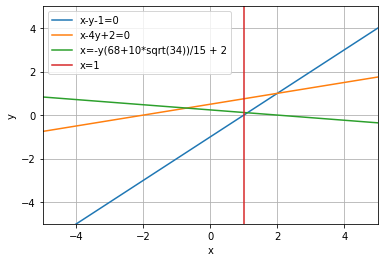
\includegraphics[width=\columnwidth]{./solutions/13/2/assignment3.png}
    \caption{Intersection of pair of original pair of straight lines and the pair of straight lines after affine transform}
    \label{eq:solutions/13/2/fig:fig1}
\end{figure}

Using \eqref{eq:solutions/13/2/eq:nvalues} and \eqref{eq:solutions/13/2/eq:cvalues} in \eqref{eq:solutions/13/2/eq:line1line2}, equation of the pair of straight lines is
\begin{align}
    (x-y-1)(x-4y+2) = 0
\end{align}

{Angle between lines}
Angle between pair of lines is,
\begin{align}\label{eq:solutions/13/2/eq:cos}
    \theta = \cos^{-1}\left(\frac{\vec{n}_1^T\vec{n}_2}{\norm{\vec{n}_1}\norm{\vec{n}_2}}\right)
\end{align}
\begin{align}
    \vec{n}_1^T\vec{n}_2 = \myvec{-1 & 1}\myvec{-1 \\ 4} = 5 \label{eq:solutions/13/2/eq:a2} 
\end{align}
\begin{align}
    \norm{\vec{n}_1}=\sqrt{(-1)^2+1^2}=\sqrt{2}\\
    \norm{\vec{n}_2}=\sqrt{(-1)^2+4^2}=\sqrt{17} \label{eq:solutions/13/2/eq:}
\end{align}
Substituting these values \eqref{eq:solutions/13/2/eq:cos}
\begin{align}
    \theta = 30.9\degree
\end{align}
Hence, angle between the given pair of straight lines is $30.9\degree$
{Affine Transformation and Eigen Value decomposition}
First, verifying if $\vec{u}^T\vec{V}^{-1}\vec{u}-f = 0$. To do this, finding $V^{-1}$ by augmenting with identity matrix and row reducing as follows :
\begin{align}
    \myvec{1 & \frac{-5}{2} & 1 & 0\\ \frac{-5}{2} & 4 & 0 & 1}\xleftrightarrow{R_2\leftarrow R_2 + \frac{5}{2}R_1}\myvec{1 & \frac{-5}{2} & 1 & 0\\ 0 & \frac{-9}{4} & \frac{5}{2} & 1}\\\xleftrightarrow{R_2\leftarrow\frac{-4}{9}R_2}\myvec{1 & \frac{-5}{2} & 1 & 0\\ 0 & 1 & \frac{-10}{9} & \frac{-4}{9}}\\\xleftrightarrow{R_1\leftarrow R_1 + \frac{5}{2}R_2}\myvec{1 & 0 & \frac{-16}{9} & \frac{-10}{9}\\ 0 & 1 & \frac{-10}{9} & \frac{-4}{9}}\\
    \implies\vec{V}^{-1} = \myvec{\frac{-16}{9} & \frac{-10}{9} \\ \frac{-10}{9} & \frac{-4}{9}}
\end{align}
\begin{align}
    u^TV^{-1}u-f & = \myvec{\frac{1}{2} & 1}\myvec{\frac{-16}{9} & \frac{-10}{9} \\ \frac{-10}{9} & \frac{-4}{9}}\myvec{\frac{1}{2} \\ 1} - (-2) \\ & = 0
\end{align}
The characteristic equation of $\vec{V}$ is given as :
\begin{align}
    \mydet{\lambda\vec{I}-\vec{V}} = \mydet{\lambda - 1 & \frac{5}{2} \\ \frac{5}{2} & \lambda - 4} = 0\\
    \implies (\lambda - 1)(\lambda - 4) - \dfrac{25}{4} = 0\\
    \label{eq:solutions/13/2/eq:characteristic}\implies 4\lambda^2-20\lambda-9 = 0
\end{align}
The roots of \eqref{eq:solutions/13/2/eq:characteristic}, i.e. the eigenvalues of $\vec{V}$ are
\begin{align}
    \lambda_1 = \dfrac{5+\sqrt{34}}{2}, \lambda_2 = \dfrac{5-\sqrt{34}}{2}\label{eq:solutions/13/2/eq:eigenval}
\end{align}
The eigen vector $\vec{p}$ is defined as, 
\begin{align}
    \vec{V}\vec{p} &= \lambda\vec{p}\\
    \implies(\lambda\vec{I}-\vec{V})\vec{p}=0
\end{align}
For $\lambda_1=\dfrac{5+\sqrt{34}}{2}$
\begin{align}
    (\lambda_1\vec{I}-\vec{V}) = \myvec{\frac{3+\sqrt{34}}{2} & \frac{5}{2} \\ \frac{5}{2} & \frac{-3 +\sqrt{34}}{2}}
\end{align}
To find $\vec{p}_1$, let's look at Augmented form of $(\lambda_1\vec{I}-\vec{V})$
\begin{align}
    \myvec{\frac{3+\sqrt{34}}{2} & \frac{5}{2} & 0 \\ \frac{5}{2} & \frac{-3 +\sqrt{34}}{2} & 0}\\\xleftrightarrow{R_1 \leftarrow \frac{2}{3+\sqrt{34}}R_1}\myvec{1 & \frac{-3+\sqrt{34}}{5} & 0 \\ \frac{5}{2} & \frac{-3 +\sqrt{34}}{2} & 0}\\\xleftrightarrow{R_2\leftarrow \frac{2}{5}R_2 - R_1}\myvec{1 & \frac{-3+\sqrt{34}}{5} & 0 \\ 0&0&0}
\end{align}
So we get
\begin{align}
    x_1 + \left(\frac{-3+\sqrt{34}}{5}\right) x_2 = 0
\end{align}
Thus, our eigenvector corresponding to $\lambda_1$
\begin{align}
    \vec{p}_1 = \myvec{\frac{3-\sqrt{34}}{5} \\ 1}
\end{align}
For $\lambda_2=\dfrac{5-\sqrt{34}}{2}$
\begin{align}
    (\lambda_2\vec{I}-\vec{V}) = \myvec{\frac{3-\sqrt{34}}{2} & \frac{5}{2} \\ \frac{5}{2} & \frac{-3 -\sqrt{34}}{2}}
\end{align}
To find $\vec{p}_2$, let's look at Augmented form of $(\lambda_2\vec{I}-\vec{V})$
\begin{align}
    \myvec{\frac{3-\sqrt{34}}{2} & \frac{5}{2} & 0 \\ \frac{5}{2} & \frac{-3 -\sqrt{34}}{2} & 0}\\\xleftrightarrow{R_1 \leftarrow \frac{2}{3-\sqrt{34}}R_1}\myvec{1 & \frac{-3-\sqrt{34}}{5} & 0 \\ \frac{5}{2} & \frac{-3 -\sqrt{34}}{2} & 0}\\\xleftrightarrow{R_2\leftarrow \frac{2}{5}R_2 - R_1}\myvec{1 & \frac{-3-\sqrt{34}}{5} & 0 \\ 0&0&0}
\end{align}
So we get
\begin{align}
    x_1 + \left(\frac{-3-\sqrt{34}}{5}\right) x_2 = 0
\end{align}
Thus, our eigenvector corresponding to $\lambda_2$
\begin{align}
    \vec{p}_2 = \myvec{\frac{3+\sqrt{34}}{5} \\ 1}
\end{align}
We know $\vec{V} = \vec{P}\vec{D}\vec{P}^{T}$, where $\vec{P}$ and the diagonal matrix $\vec{D}$ are given as:
\begin{align}
    \vec{D} & = \myvec{\lambda_1 & 0 \\ 0 & \lambda_2}\\ & = \myvec{\frac{5+\sqrt{34}}{2} & 0\\ 0 & \frac{5-\sqrt{34}}{2}}\label{eq:solutions/13/2/eq:DVal}\\
    \vec{P} & = \myvec{\vec{p}_1 & \vec{p}_2}\\&= \myvec{\frac{3-\sqrt{34}}{5} & \frac{3+\sqrt{34}}{5}\\ 1 & 1}\label{eq:solutions/13/2/eq:PVal}
\end{align}
So, the equation of the pair of straight lines is given by :
\begin{align}
    \vec{y}^T\vec{D}\vec{y} = \vec{u}^T\vec{V}^{-1}\vec{u}-f\qquad\text{$\mydet{\vec{V}}\neq0$}\\
    \vec{y}^T\myvec{\dfrac{5+\sqrt{34}}{2} & 0\\ 0 & \dfrac{5-\sqrt{34}}{2}}\vec{y} =0\\
    \implies \myvec{y_1 & y_2}\myvec{\dfrac{5+\sqrt{34}}{2} & 0\\ 0 & \dfrac{5-\sqrt{34}}{2}}\myvec{y_1 \\ y_2} = 0\\
    \implies (5+\sqrt{34})y_1^2 + (5-\sqrt{34})y_2^2 = 0
\end{align}
So we get the equation of the pair of straight lines, as we can see this passes through the origin $(0,0)$. The corresponding image is shown in Fig. \ref{eq:solutions/13/2/fig:fig2}
\begin{align}
    \vec{c} = -\vec{V}^{-1}\vec{u}\qquad\text{$\mydet{\vec{V}}\neq0$}\\
    \implies \vec{c} = -\myvec{\frac{-16}{9} & \frac{-10}{9} \\ \frac{-10}{9} & \frac{-4}{9}}\myvec{\frac{1}{2} \\ 1} = \myvec{2 \\ 1}\\
    \intertext{And,}
    \vec{P}^T = \myvec{\frac{3-\sqrt{34}}{5} & 1\\ \frac{3+\sqrt{34}}{5} & 1}
    \intertext{Using affine transformation, we can express the equation as}
    \vec{x} = \vec{P}\vec{y} + \vec{c}\\
    \implies \vec{x} = \myvec{\frac{3-\sqrt{34}}{5} & \frac{3+\sqrt{34}}{5}\\1 & 1}\vec{y} + \myvec{2 \\ 1}
\end{align}
The corresponding image is shown in Fig. \ref{eq:solutions/13/2/fig:fig1}
\begin{figure}[h!]
    \centering
    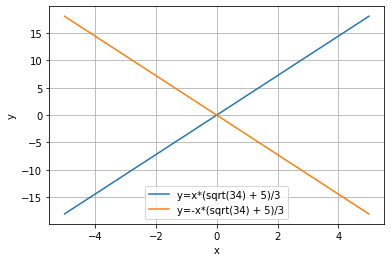
\includegraphics[width=\columnwidth]{./solutions/13/2/assignment3.1.png}
    \caption{Pair of straight lines passing through origin after eigenvalue decomposition}
    \label{eq:solutions/13/2/fig:fig2}
\end{figure}

\item Prove that the following equations represent two straight lines.Also find their point of intersection and the angle between them
\begin{align}
 3y^2-8xy-3x^2-29x+3y-18=0   
\label{eq:solutions/13/3/1}
\end{align}
\solution
\mydet{\vec{V}&\vec{u}\\\vec{u}^T&f} of \eqref{eq:solutions/13/3/1} becomes
\begin{align}
    \mydet{-3&-4&-\frac{29}{2}\\-4&3&\frac{3}{2}\\-\frac{29}{2}&\frac{3}{2}&-18}\label{eq:solutions/13/3/2}
\end{align}
Expanding equation \eqref{eq:solutions/13/3/2}, we get zero.\\
Hence given equation represents a pair of straight lines.
Slopes of the individual lines are roots of equation 
\begin{align}
    cm^2+2bm+a=0\\
    \implies 3m^2-8m-3=0\\
    \text{Solving, }m=3,-\frac{1}{3}
\end{align}
The normal vectors of the lines then become
\begin{align}
    \vec{n_1}=\myvec{\frac{1}{3}\\1}\\
    \vec{n_2}=\myvec{-3\\1}
\end{align}
Equations of the lines can therefore be written as
\begin{align}
  \myvec{\frac{1}{3}&1}\vec{x}=c\\
 \implies \myvec{1&3}\vec{x}=c_1 ,\\
   \myvec{-3&1}\vec{x}=c_2\\
  \implies \left[\myvec{1&3}\vec{x}-c_1\right]\left[\myvec{-3&1}\vec{x}-c_2\right]
\end{align}
represents the equation specified in \eqref{eq:solutions/13/3/1}\\
Comparing the equations, we have
\begin{align}
    \myvec{1&-3\\3&1}\myvec{c_2\\c_1}=\myvec{29\\-3}\\
 \end{align}
 Row reducing the augmented matrix
 \begin{align}
    \myvec{1&-3&29\\3&1&-3}\xleftrightarrow[]{R_2\leftarrow R_2-3\times R_1}
    \myvec{1&-3&29\\0&10&-90}\\
    \xleftrightarrow[]{R_2\leftarrow R_2\times \frac{1}{10}}
    \myvec{1&-3&29\\0&1&-9}\\
    \xleftrightarrow[]{R_1\leftarrow R_1+3\times R_2}
    \myvec{1&0&2\\0&1&-9}\\
    \implies c_2=2 \text{ and }c_1=-9
\end{align}
The individual line equations therefore become
\begin{align}
    \myvec{1&3}\vec{x}=-9\label{eq:solutions/13/3/3} ,\\\myvec{-3&1}\vec{x}=2\label{eq:solutions/13/3/4}
\end{align}
Note that the convolution of the normal vectors, should satisfy the below condition
\begin{align}
    \myvec{1\\3}*\myvec{-3\\1}=\myvec{a\\2b\\c}\label{eq:solutions/13/3/5}
\end{align}
The LHS part of \eqref{eq:solutions/13/3/5} can be rewritten using toeplitz matrix as
\begin{align}
    \myvec{1&0\\3&1\\0&3}\myvec{-3\\1}=\myvec{-3\\-8\\3}=\myvec{a\\2b\\c}
\end{align}

The augmented matrix for the set of equations represented in \eqref{eq:solutions/13/3/3}, \eqref{eq:solutions/13/3/4} is
\begin{align}
\myvec{1&3&-9\\-3&1&2}
\end{align}
Row reducing the matrix
\begin{align}
 \myvec{1&3&-9\\-3&1&2}\xleftrightarrow[]{R_2\leftarrow R_2+3\times R_1}\myvec{1&3&-9\\0&10&-25}\\
 \xleftrightarrow[]{R_1\leftarrow R_1-\frac{3}{10}\times R_2}\myvec{1&0&-\frac{3}{2}\\0&10&-25}\\
 \xleftrightarrow[]{R_2\leftarrow \frac{R_2}{10}}\myvec{1&0&-\frac{3}{2}\\0&1&-\frac{5}{2}}\\
\text{Hence, the intersection point is}
\myvec{-\frac{3}{2}\\-\frac{5}{2}}
\end{align}
\begin{figure}[!ht]
\centering
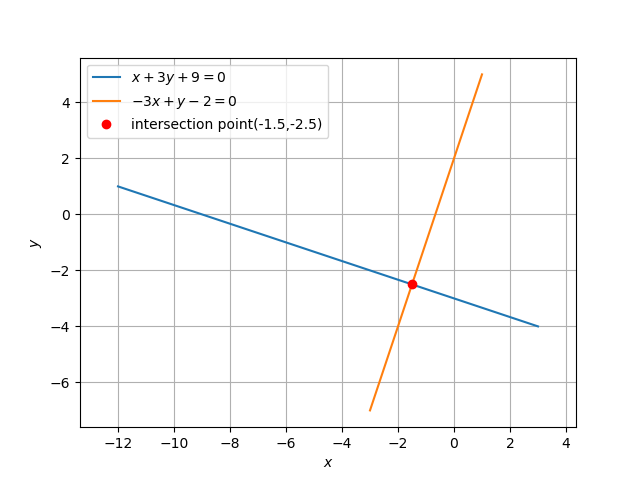
\includegraphics[width=\columnwidth]{./solutions/13/3/hw4plot.png}
\caption{plot showing intersection of lines}
\label{eq:solutions/13/3/Fig:solutions/13/3/}
\end{figure}
Angle between two lines $\theta$ can be given by
\begin{align}
\cos \theta = \frac{\vec{n_1}^T\vec{n_2}}{\norm{\vec{n_1}}\norm{\vec{n_2}}}
\end{align}
%From \eqref{eq:solutions/13/3/3}, \eqref{eq:solutions/13/3/4},
\begin{align}
\cos \theta=\frac{\myvec{1&3}\myvec{-3\\1}}{\sqrt{(3)^2 +1} \times \sqrt{(-3)^2 +1}}=0\\
\implies \theta = 90\degree
\end{align}


\item Prove that the following equations represents two straight lines also find their point of intersection and angle between them.
\begin{align}
y^2+xy-2x^2-5x-y-2=0
\end{align}
%
\solution
\begin{align}
\vec{V}=\myvec{a&b\\b&c}=\myvec{-2&\frac{1}{2}\\\frac{1}{2}&1}\\
\vec{u}=\myvec{d\\e}=\myvec{\frac{-5}{2}\\\frac{-1}{2}}\\
f=-2
\end{align}
\begin{align}
\mydet{
-2&\frac{1}{2}&\frac{-5}{2}\\
\frac{1}{2}&1&\frac{-1}{2}\\
\frac{-5}{2}&\frac{-1}{2}&-2}
\xleftrightarrow[R_1\rightarrow R_1+R_3]{R_1\rightarrow R_1-R_2}
\mydet{
0&0&0\\
\frac{1}{2}&1&\frac{-1}{2}\\
\frac{-5}{2}&\frac{-1}{2}&-2}=0
\end{align}
Hence it represents the pair of straight lines.
Now two intersecting lines are obtained when
\begin{align}
\mydet{V} < 0 
\implies \mydet{-2&\frac{1}{2}\\\frac{1}{2}&1}
=\frac{-9}{4} < 0
\end{align}
Let the pair of straight of lines be given by
\begin{align}
\vec{n_1}^T\vec{x}=c_1\\
\vec{n_2}^T\vec{x}=c_2
\end{align}
The slopes of the lines are given by the roots of the polynomial 
\begin{align}
cm^2+2bm+a=0 \\
m_1,m_2 = \frac{-\frac{1}{2}\pm\sqrt{\frac{9}{4}}}{1}\\
m_1= 1 , m_2 =-2\\
\implies\vec{n_1}=\myvec{-1\\1} and \vec{n_2}=\myvec{2\\1}
\end{align}
\begin{align}
(\vec{n_1}^T\vec{x}-c_1)(\vec{n_2}^T\vec{x}-c_2) =
\vec{x}^T\vec{V}\vec{x}+2\vec{u}^T\vec{x}+f 
\end{align}
\begin{align}
c_2\vec{n_1}+c_1\vec{n_2} =-2\vec{u}
 \end{align}
 \begin{align}
 c_2\myvec{-1\\1}+c_1\myvec{2\\1} =-2\myvec{\frac{-5}{2}\frac{-1}{2}}
 \end{align}
 \begin{align}
 \myvec{1&1\\2&-1}\myvec{c_1\\c_2}=\myvec{1\\5}
 \end{align}
 Using row reduction we get
 \begin{align}
\myvec{1&1&1\\2&-1&5}\\
\xleftrightarrow[R_2\leftarrow R_2/-3]{R_2\leftarrow R_2-2R_1}
\myvec{1&1&1\\0&1&-1}\\\xleftrightarrow[]{R_1\leftarrow R_1-R_2}
\myvec{1&0&2\\0&1&-1}
\end{align}
\begin{align}
C  =\myvec{2\\-1}
\end{align}
 The convolution of the normal vectors, should satisfy the below condition
 \begin{align}
    \myvec{-1\\1}*\myvec{2\\1}=\myvec{a\\2b\\c}
\end{align}
The LHS part of equation(2.0.20) can be rewritten using toeplitz matrix as
\begin{align}
    \myvec{-1&0\\1&-1\\0&1}\myvec{2\\1}=\myvec{-2\\1\\1}=\myvec{a\\2b\\c}
\end{align}
Therefore the equation of lines is given by 
\begin{align}
\myvec{-1&1}\vec{x}=2\\
\myvec{2&1}\vec{x}=-1
\end{align}
consider the augmented matrix
\begin{align}
\myvec{-1&1&2\\2&1&-1}\\
\xleftrightarrow[R_2\leftarrow R_2-2R_1]{R_1\leftarrow -R_1}
\myvec{1&2&1\\0&1&1}\\\xleftrightarrow[R_1\leftarrow R_1+R_2]{R_1\leftarrow R_1/3}
\myvec{1&0&-1\\0&1&1}
\end{align}
Therefore point of intersection is $\vec{A}=\myvec{-1\\1}.$
\\
Angle between two lines $\theta$ can be given by
\begin{align}
\cos\theta =\frac{\vec{n_1}^T\vec{n_2}}{\norm{\vec{n_1}}\norm{\vec{n_2}}}\\
 \cos\theta=\frac{\myvec{-1&1}\myvec{2\\1}}{\sqrt{\left(1\right)^2 +1} \times \sqrt{(2)^2 +1}}
\end{align}
\begin{align}
\theta = \cos^{-1}(\frac{-1}{\sqrt{10}})\implies \theta = tan^{-1}3
\end{align}
\begin{figure}[!ht]
\centering
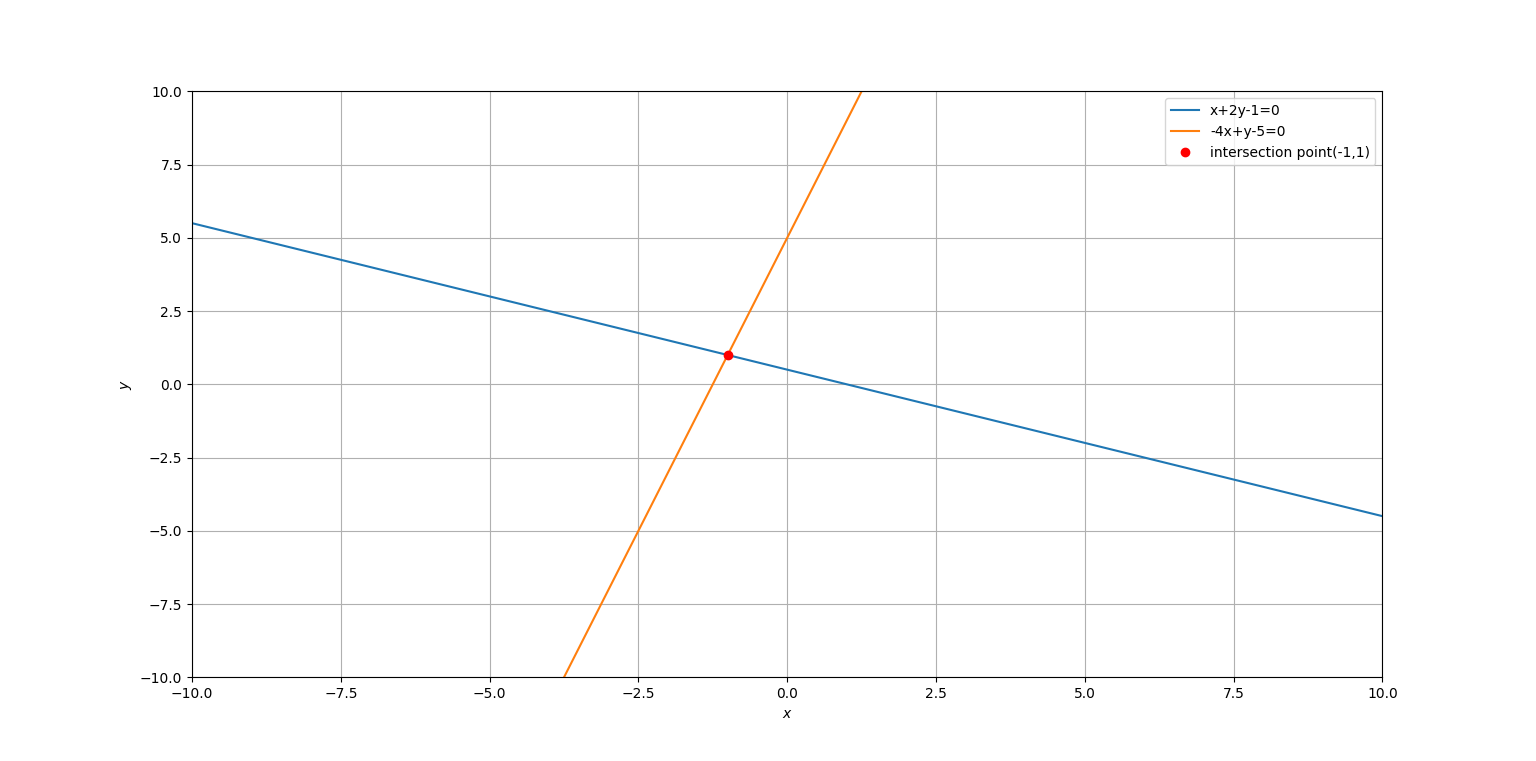
\includegraphics[width=\columnwidth]{./solutions/13/4/Figure_2.png}
\caption{plot showing intersection of lines}
\label{Fig:solutions/13/4}
\end{figure}

\item Prove that the equation
\begin{align} 
    x^{2}+6xy+9y^{2}+4x+12y-5=0 \label{eq:solutions/13/5/eq:0}
\end{align}
represents two parallel lines.

\solution
The given equation \eqref{eq:solutions/13/5/eq:0} can be written as
\begin{align}
\vec{x}^T\myvec{1 & 3 \\ 3 & 9}\vec{x} +2\myvec{2 &6}\vec{x}-5=0\label{eq:solutions/13/5/eq:1}\\
\vec{V} = \myvec{1 & 3 \\ 3 & 9} \quad \vec{u} = \myvec{2 \\ 6} \quad f= -5 \label{eq:solutions/13/5/eq:2}
\end{align}
Equation \eqref{eq:solutions/13/5/eq:0} represents pair of straight line as,
\begin{align}
D = \mydet{1&3&2\\3&9&6\\2&6&-5} = 0
\end{align}
Vector form of straight lines,
\begin{align}
\vec{n_1}^T\vec{x}= \vec{c_1}\\
\vec{n_2}^T\vec{x} = \vec{c_2}
\end{align}
Equating their product with \eqref{eq:solutions/13/5/eq:1}
\begin{align}
(\vec{n_1}^T\vec{x} -\vec{c_1})(\vec{n_2}^T\vec{x} - \vec{c_2})= \vec{x}^T\myvec{1 & 3 \\ 3 & 9}\vec{x} +2\myvec{2 &6}\vec{x}-5
\end{align}
\begin{align}
\vec{n_1}*\vec{n_2}=\myvec{1\\6\\9}\label{eq:solutions/13/5/eq:3}\\
c_2\vec{n_1}+c_1\vec{n_2} = -2\myvec{2\\6}\\
c_1c_2 = -5
\end{align}
The slopes of the lines can be given by roots of the equation,
\begin{align} 
cm^2+2bm+a=0 \label{eq:solutions/13/5/eq:4}\\
m_i = \frac{-b\pm \sqrt{-\mydet{\vec{V}}}}{c}\label{eq:solutions/13/5/eq:5}\\
\vec{n_i}=k_i\myvec{-m_i\\1}\label{eq:solutions/13/5/eq:6}
\end{align}
From \eqref{eq:solutions/13/5/eq:1} equation \eqref{eq:solutions/13/5/eq:4} becomes
\begin{align}
9m^2+6m+1=0
\end{align}
Using \eqref{eq:solutions/13/5/eq:2},
\begin{align}
\mydet{\vec{V}} = \mydet{1 & 3\\ 3 & 9} = 0
\end{align}
Substituting the values in \eqref{eq:solutions/13/5/eq:5},
\begin{align}
m_i = \frac{-3\pm 0}{9}\\
m_1= m_2 = \frac{-1}{3} \label{eq:solutions/13/5/eq:7}
\end{align}
Substituting values in \eqref{eq:solutions/13/5/eq:6}
\begin{align}
\vec{n_1}=k_1\myvec{\frac{1}{3}\\1}\\
\vec{n_2}=k_2\myvec{\frac{1}{3}\\1}
\end{align}
Using the above values in \eqref{eq:solutions/13/5/eq:3},
\begin{align}
k_1k_2 = 9
\end{align}
Taking $k_1=3$ and $k_2 = 3$ we get
\begin{align}
\vec{n_1}=\myvec{1\\3}\\
\vec{n_2}=\myvec{1\\3}
\end{align}
Verifying $\vec{n_1}$ and $\vec{n_2}$ by computing the convolution by representing $\vec{n_1}$ as Toeplitz matrix,
\begin{align}
\vec{n_1}*\vec{n_2}=\myvec{1&0\\3&1\\0&3}\myvec{1\\3}=\myvec{1\\6\\9}
\end{align}
Finding the Angle between the lines,
\begin{align}
\theta = \cos^{-1}\brak{\frac{\vec{n_1}^T\vec{n_2}}{\norm{\vec{n_1}}\norm{\vec{n_2}}}}\label{eq:solutions/13/5/eq:8}\\
\vec{n_1}^T\vec{n_2} = \myvec{1&3}\myvec{1\\3} = 10 \label{eq:solutions/13/5/eq:9}\\
\norm{\vec{n_1}} = \sqrt{10}\quad \norm{\vec{n_2}}=\sqrt{10} \label{eq:solutions/13/5/eq:10}
\end{align}
Substituting \eqref{eq:solutions/13/5/eq:9} and \eqref{eq:solutions/13/5/eq:10} in \eqref{eq:solutions/13/5/eq:8} we get,
\begin{align}
\theta = \cos^{-1}(1)\\
\theta = 0^{\circ}\label{eq:solutions/13/5/eq:11}
\end{align}
From \eqref{eq:solutions/13/5/eq:7} and \eqref{eq:solutions/13/5/eq:11} shows the given equation \eqref{eq:solutions/13/5/eq:0} represents two parallel lines. Hence proved.
\begin{figure}[!ht]
\centering
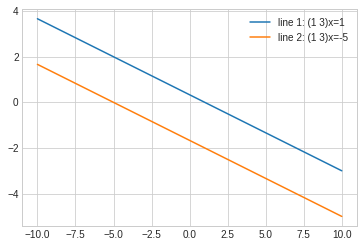
\includegraphics[width=\columnwidth]{./solutions/13/5/Straight_lines.png}
\caption{Pair of straight lines plot generated using python}
\label{eq:solutions/13/5/fig:plot}
\end{figure}

\item 
%
\solution
Find the value of k such that 
\begin{align}
	6x^2 + 11xy - 10y^2 + x + 31y + k =0 \label{eq:solutions/13/6/eq:eq5}
\end{align}

represent pairs of straight lines.

From \eqref{eq:solutions/13/6/eq:eq5} we get,
\begin{align}
	\vec{V} &= \myvec{6 & \frac{11}{2} \\ \frac{11}{2} & -10}\\
	\vec{u} &= \myvec{\frac{1}{2}\\ \frac{31}{2}}\\
	f &= k
\end{align}
Compute the slopes of lines given by the roots of the polynomial $-10m^2 + 11m + 6$
\begin{align}
   i.e., m_i &= \frac{-b \pm \sqrt{- \mydet{\vec{V}}}}{c} \label{eq:solutions/13/6/eq:eq2} \\
   \implies m &= \frac{\frac{-11}{2} \pm \frac{19}{2}}{-10} \\ 
   \implies m_1 &= \frac{-2}{5}, m_2 = \frac{3}{2} 
\end{align} 
Let the pair of straight lines be given by 
\begin{align}
	\vec{n}_1^T\vec{x} = c_1 \label{eq:solutions/13/6/eq:n_1}\\
	\vec{n}_2^T\vec{x} = c_2 \label{eq:solutions/13/6/eq:n_2}
\end{align}
Here,
\begin{align}
	\vec{n}_1 &= k_1\myvec{-m_1\\1} = k_1 \myvec{ \frac{2}{5} \\ 1}  \label{eq:solutions/13/6/eq:n1val}\\
	\vec{n}_2 &= k_2\myvec{-m_2\\1} = k_2 \myvec{\frac{-3}{2} \\ 1} \label{eq:solutions/13/6/eq:n2val}
\end{align}
We know that, 
\begin{align}
	\vec{n}_1 * \vec{n}_2 = \myvec{a\\2b\\c} \label{eq:solutions/13/6/eq:n1n2}
\end{align}
Substituting \eqref{eq:solutions/13/6/eq:n1val} and \eqref{eq:solutions/13/6/eq:n2val} in the above equation, we get
\begin{align}
	k_1 \myvec{ \frac{2}{5} \\ 1} * k_2 \myvec{\frac{-3}{2} \\ 1} &= \myvec{6\\ 11\\ -10}\\
	\implies k_1k_2 &= -10
\end{align} 
By inspection, we get the values, $k_1 = 5, k_2 = -2$. Substituting the values of $k_1$ and $k_2$ in \eqref{eq:solutions/13/6/eq:n1val} and \eqref{eq:solutions/13/6/eq:n2val} respectively, we get
\begin{align}
	\vec{n}_1 &= \myvec{2 \\ 5} \label{eq:solutions/13/6/eq:n1}\\
	\vec{n}_2 &= \myvec{3 \\ -2} \label{eq:solutions/13/6/eq:n2}
\end{align}
Using Teoplitz matrix representation, the convolution of $\vec{n}_1$ with $\vec{n}_2$, is as follows:
\begin{align}
	\myvec{2 & 0 & 5\\ 5 & 2 & 0\\ 0 & 5 & 2}\myvec{3\\-2\\0} = \myvec{6 \\11 \\ -10} = \myvec{a \\ 2b \\ c}
\end{align}
Hence, $\vec{n}_1$ and $\vec{n}_2$ satisfies \eqref{eq:solutions/13/6/eq:n1n2}.
We have,
\begin{align}
	c_2\vec{n}_1 + c_1\vec{n}_2 &= -2\vec{u} \label{eq:solutions/13/6/eq:cneq}
\end{align}
Substituting \eqref{eq:solutions/13/6/eq:n1}, \eqref{eq:solutions/13/6/eq:n2} in \eqref{eq:solutions/13/6/eq:cneq}, we get
\begin{align}
 \myvec{2 & 3\\ 5 & -2}\myvec{c_2 \\ c_1} &= -2\myvec{\frac{1}{2} \\ \frac{31}{2}}
\end{align}
Solving for $c_1$ and $c_2$, the augmented matrix is,
\begin{align}
	\myvec{2 & 3 & -1\\ 5 & -2 & -31} &\xleftrightarrow[R_2 \leftarrow R_2 - 5R_1]{R_1 \leftarrow \frac{R_1}{2}} \myvec{1 & \frac{3}{2}  & \frac{-1}{2} \\ 0 & \frac{-19}{2} & \frac{-57}{2}} \\
	&\xleftrightarrow[R_1 \leftarrow R_1 - \frac{3}{2}R_2]{R_2 \leftarrow \frac{R_2}{-19/2}} \myvec{1 & 0 & -5\\0 & 1 & 3}
\end{align}
Hence we obtain,
\begin{align}
	c_1 = 3, c_2 = -5
\end{align}
We know that,
\begin{align}
	f = k = c_1c_2\\
	\implies \boxed{k = -15}
\end{align}
Hence the solution. Using \eqref{eq:solutions/13/6/eq:n_1} and \eqref{eq:solutions/13/6/eq:n_2}, the equation of pair of straight lines is given by,
\begin{align}
\myvec{2 & 5}\vec{x} &= 3\\
\myvec{3 & -2}\vec{x} &= -5
\end{align}
See Fig. \ref{fig:solutions/13/6/}


\begin{figure}[!ht] 
	\centering
	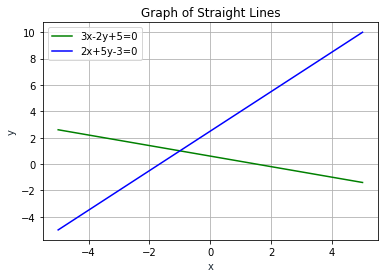
\includegraphics[width=\columnwidth]{./solutions/13/6/a6_graph.png}
	\caption{Plot of two straight lines.}
\label{fig:solutions/13/6/}
\end{figure}

%
\item Find the value of k so that following equation may represent pairs of straight lines,
\begin{align}
12x^2-10xy+2y^2+11x-5y+k=0
\label{eq:solutions/13/7/1}
\end{align}
%
\solution
The general equation of second degree is given by,
\begin{align}
ax^2 + 2bxy + cy^2 + 2dx +2ey +f = 0
\label{eq:solutions/13/7/2}
\end{align}
In vector from the equation \eqref{eq:solutions/13/7/2} can be expressed as,
\begin{align}
\vec{x}^T\vec{V}\vec{x} + 2\vec{u}^T\vec{x} + f = 0 
\label{eq:solutions/13/7/line_vec}
\end{align}
where,
\begin{align}
\vec{V} = \vec{V}^T = \myvec{a&b\\b&c}
\label{eq:solutions/13/7/3}
\end{align}
\begin{align}
\vec{u} = \myvec{d\\e}
\label{eq:solutions/13/7/4}
\end{align}
Now, comparing \eqref{eq:solutions/13/7/2} to \eqref{eq:solutions/13/7/1} we get, a =12, b=-5, c = 2, d = $\frac{11}{2}$,e = -$\frac{5}{2}$, f = k.  
Hence, substituting these values in \eqref{eq:solutions/13/7/3} and \eqref{eq:solutions/13/7/4} we get,
\begin{align}
\vec{V} = \myvec{12 & -5 \\ -5 & 2}
\end{align}
\begin{align}
\vec{u} = \myvec{\frac{11}{2} \\ -\frac{5}{2}}
\end{align}
\eqref{eq:solutions/13/7/1} represents pair of straight lines if,
\begin{align}
\mydet{\vec{V}&\vec{u}\\\vec{u}^T&f} = 0
\end{align}
\begin{align}
\mydet{12&-5&\frac{11}{2}\\-5&2&-\frac{5}{2}\\\frac{11}{2}&-\frac{5}{2}&k} = 0
\end{align}
\begin{align}
\implies k =2
\label{eq:solutions/13/7/5}
\end{align}
Lines Intercept if
\begin{align}
    |\vec{V}|<0\\
    |\vec{V}|=-1<0
\end{align}
Hence Line intercept.\\
Let $(\alpha,\beta)$ be their point of intersection, then
\begin{equation}\label{eq:solutions/13/7/eq6}
	\myvec{ a & b\\ b & c}\myvec{\alpha \\ \beta} = \myvec{-d \\ -e}
\end{equation}
Substituting in \eqref{eq:solutions/13/7/eq6}
\begin{align}
	\label{eq:solutions/13/7/eq11}\myvec{ 12 & -5\\-5 & 2}\myvec{\alpha \\ \beta} = \myvec{-\frac{11}{2} \\ \frac{5}{2}} \\
	\label{eq:solutions/13/7/eq12}\implies \myvec{\alpha \\ \beta} = \myvec{-\frac{3}{2} \\ -\frac{5}{2}}
\end{align}
Spectral Decomposition  of $\vec{V}$ is given as
\begin{equation}
\vec{V} = \vec{P}\vec{D}\vec{P}^T
\end{equation}
\begin{align}
	\label{eq:solutions/13/7/eq7}\vec{V} &= \myvec{ 12 & -5\\ -5 & 2}\\
	\label{eq:solutions/13/7/eq8}\vec{P} &= \myvec{-1-\sqrt{2} & -1 + \sqrt{2}\\ 1 & 1}\\
	\label{eq:solutions/13/7/eq9}\vec{D} &= \myvec{7 + 5\sqrt{2} & 0\\ 0 & 7 - 5\sqrt{2}}
\end{align}
Using Spectral decomposition concept and substution
\begin{align}
u_1(x-\alpha) + u_2(y-\beta) &= \pm \sqrt{-\frac{\lambda_2}{\lambda_1}}(v_1(x-\alpha) + v_2(y-\beta))\label{eq:solutions/13/7/eq10}
\end{align}
Substituting \eqref{eq:solutions/13/7/eq12}, \eqref{eq:solutions/13/7/eq8} and \eqref{eq:solutions/13/7/eq9} in \eqref{eq:solutions/13/7/eq10}
\begin{multline}\label{eq:solutions/13/7/eq13}
	\brak{-1-\sqrt{2}}\brak{x- \frac{-3}{2}} + \brak{y-\frac{-5}{2}} \\= \pm \sqrt{-\frac{7 +5\sqrt{2}} {7-5\sqrt{2}}}\brak{\brak{-1+\sqrt{2}}\brak{x- \frac{-3}{2}} + \brak{y-\frac{-5}{2}}}
\end{multline}
Simplifying \eqref{eq:solutions/13/7/eq13},
\begin{align}
	\label{eq:solutions/13/7/eq22}-6x + 2y - 4 = 0 \text{ and } -2x + y -\frac{1}{2} = 0\\
	\implies \brak{-6x + 2y - 4}\brak{-2x + y -\frac{1}{2}} = 0
\end{align}
Thus the equation of lines are
\begin{align}
\myvec{-6&2}\vec{x} = 4\\ 
\myvec{-2&1}\vec{x} = \frac{1}{2}
\end{align}
Hence, Plot is shown below 
\begin{figure}[ht!]
\centering
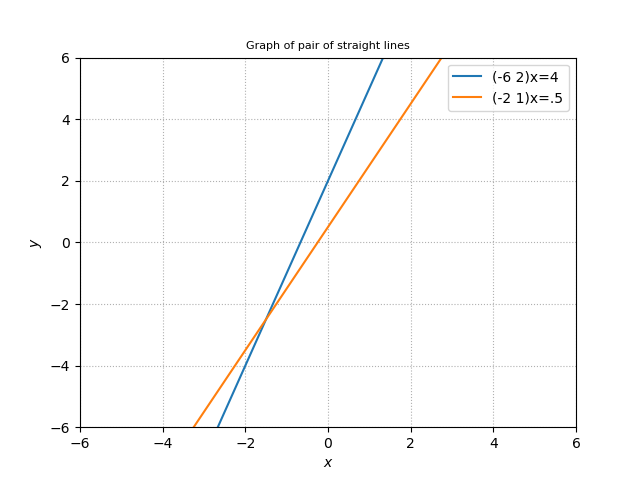
\includegraphics[width=\columnwidth]{./solutions/13/7/Figure.png}
\caption{Pair of lines}
\end{figure}

\item Find the value of k so that the following equation may represent pair of straight lines: 
\begin{align}
    12x^2+kxy+2y^2+11x-5y+2=0\label{eq:solutions/13/8/1.1}
\end{align}
\solution
\begin{align}
    \vec{V}=\vec{V}^T=\myvec{a & b \\ b & c}=\myvec{12 & \frac{k}{2} \\ \frac{k}{2} & 2}\label{eq:solutions/13/8/2.3}\\
    \vec{u}=\myvec{d \\ e}=\myvec{\frac{11}{2} \\ -\frac{5}{2}}\label{eq:solutions/13/8/2.4}
\end{align}

The equation \eqref{eq:solutions/13/8/1.1} represents pair of straight lines if
\begin{align}
    &\mydet{\vec{V} & \vec{u} \\ \vec{u}^T & f}=0\\
    \implies&\mydet{12 & \frac{k}{2} & \frac{11}{2} \\ \frac{k}{2} & 2 & -\frac{5}{2} \\ \frac{11}{2} & -\frac{5}{2} & 2}=0\label{eq:solutions/13/8/2.6}\\
    \implies&\mydet{24 & k & 11 \\ k & 4 & -5 \\ 11 & -5 & 4}=0\\
    \implies&24\mydet{ 4 & -5 \\ -5 & 4}-k\mydet{ k & -5 \\ 11 & 4}+11\mydet{ k & 4 \\ 11 & -5}=0
\end{align}
\begin{align}
    \implies2k^2+55k+350=0\\
    \implies(10+k)(2k+35)=0\\
    \implies k=-10\nonumber\\
    k=-\frac{35}{2}
\end{align}
Therefore, for $k=-10$ and $k=-\frac{35}{2}$ the given equation represents pair of straight lines.\\
Now Lets find equation of lines for $k=-10$.
\noindent
Substitute $k=-10$ in \eqref{eq:solutions/13/8/1.1}. We get equation of pair of straight lines as:
\begin{align}
    12x^2-10xy+2y^2+11x-5y+2=0
\end{align}
%Comparing above equation with \eqref{eq:solutions/13/8/2.1}, we will get $a=12$, $b=-5$, $c=2$, $d=\frac{11}{2}$, $e=-\frac{5}{2}$, $f=2$.\\
From \eqref{eq:solutions/13/8/1.1}, \eqref{eq:solutions/13/8/2.3}, \eqref{eq:solutions/13/8/2.4} we get
\begin{align}
    \vec{V}=\vec{V}^T=\myvec{12 & -5 \\ -5 & 2}\label{eq:solutions/13/8/2.17}\\
    \vec{u}=\myvec{\frac{11}{2} \\ -\frac{5}{2}}\label{eq:solutions/13/8/2.18}
\end{align}
\noindent
If $\mydet{\vec{V}}<0$ then two lines will intersect.
\begin{align}
    \mydet{\vec{V}}&=\mydet{12 & -5 \\ -5 & 2}\\
    \implies\mydet{\vec{V}}&=-1\\
    \implies\mydet{\vec{V}}&<0
\end{align}
\noindent
Therefore the lines will intersect.\\
The equation of two lines is given by
\begin{align}
    \vec{n_1}^T\vec{x}=c_1\label{eq:solutions/13/8/1.12}\\
    \vec{n_2}^T\vec{x}=c_2\label{eq:solutions/13/8/1.13}
\end{align}
Equating their product with \eqref{eq:solutions/13/8/1.1}
\begin{multline}
    (\vec{n_1}^T\vec{x}-c_1)(\vec{n_2}^T\vec{x}-c_2)\\=\vec{x}^T\vec{V}\vec{x}+2\vec{u}^T\vec{x}+f=0
\end{multline}
\begin{align}
    \implies\vec{n_1}*\vec{n_2}&=\myvec{a \\ 2b \\c}=\myvec{12\\-10\\2}\label{eq:solutions/13/8/conv}
\end{align}
\begin{align}
    c_2\vec{n_1}+c_1\vec{n_2}&=-2\vec{u}=-2\myvec{\frac{11}{2} \\ -\frac{5}{2}}\label{eq:solutions/13/8/1.16}\\
    c_1c_2&=f=2
\end{align}
The slopes of the lines are given by roots of equation
\begin{align}
    cm^2+2bm+a=0\label{eq:solutions/13/8/poly}\\
    \implies 2m^2-10m+12=0\\
    m_i=\frac{-b\pm{\sqrt{-\mydet{\vec{V}}}}}{c}\\
    \implies m_i=\frac{5\pm{\sqrt{1}}}{2}\\
    \implies m_1=3\\
     m_2=2
\end{align}
The normal vector for two lines is given by
\begin{align}
    \vec{n_i}=k_i\myvec{-m_i\\1}\label{eq:solutions/13/8/normvec}\\
    \implies\vec{n_1}=k_1\myvec{-3\\1}\label{eq:solutions/13/8/n1}\\
    \vec{n_2}=k_2\myvec{-2\\1}\label{eq:solutions/13/8/n2}
\end{align}
Substituting \eqref{eq:solutions/13/8/n1},\eqref{eq:solutions/13/8/n2} in \eqref{eq:solutions/13/8/conv}. we get
\begin{align}
    k_1k_2=2
\end{align}
The possible combinations of ($k_1$,$k_2$) are (1,2), (2,1), (-1,-2) and (-2,-1).\\
lets assume $k_1=1$,$k_2=2$ we get
\begin{align}
    \implies\vec{n_1}=\myvec{-3\\1}\label{soln1}\\
    \vec{n_2}=\myvec{-4\\2}\label{soln2}
\end{align}
We verify obtained $\vec{n_1}$,$\vec{n_2}$ using Toeplitz matrix
\begin{align}
    \vec{n_1}*\vec{n_2}=\myvec{-3 & 0\\1 & -3\\0 & 1}\myvec{-4 \\ 2}=\myvec{12\\-10\\2}\label{eq:solutions/13/8/comp1}\\
    \implies \vec{n_1}*\vec{n_2}=\myvec{12\\-10\\2}=\myvec{a\\2b\\c}
\end{align}
Therefore the obtained $\vec{n_1}$,$\vec{n_2}$ are correct.\\
Substitute \eqref{soln1}, \eqref{soln2} in \eqref{eq:solutions/13/8/1.16}
and calculate for $c_1$ and $c_2$

\begin{align}
    c_2\myvec{-3\\1}+c_1\myvec{-4\\2}=\myvec{ -11\\ -5}
\end{align}
Solve using row reduction technique.
\begin{align}
    \implies\myvec{-4 & -3 & -11\\2 & 1 & -5}\\
    \xleftrightarrow[]{R_2\leftarrow 2R_2+R_1}\myvec{-4 & -3 & -11\\0 & -1 & -21}\\
    \xleftrightarrow[]{R_1\leftarrow R_1-3R_2}\myvec{-4 & 0 & 52\\0 & -1 & -21}\\
    \implies\myvec{1 & 0 & -13\\0 & 1 & 21}\\
    \implies c_1=-13\label{c1}\\
    c_2=21\label{c2}
\end{align}

Substituting \eqref{soln1},\eqref{soln2},\eqref{c1},\eqref{c2} in \eqref{eq:solutions/13/8/1.12} and \eqref{eq:solutions/13/8/1.13}. We get equation of two straight lines.
\begin{align}
    \myvec{-3 & 1}\vec{x}=-13\\
    \myvec{-4 & 2}\vec{x}=21
\end{align}

The plot of these two lines is shown in Fig.~\ref{fig:solutions/13/8/figure1}.
\begin{figure}[ht!]
    \centering
    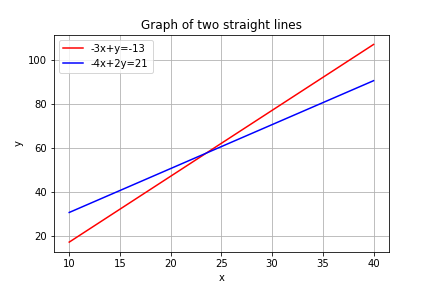
\includegraphics[width=\columnwidth]{./solutions/13/8/Figure1}
    \caption{Pair of straight lines for $k=-10$}
    \label{fig:solutions/13/8/figure1}
\end{figure}

Now Lets find equation of lines for $k=-\frac{35}{2}$.

Substitute $k=-\frac{35}{2}$ in \eqref{eq:solutions/13/8/1.1}. We get equation of pair of straight lines as:
\begin{align}
    12x^2-\frac{35}{2}xy+2y^2+11x-5y+2=0
\end{align}

%Comparing above equation with \eqref{eq:solutions/13/8/2.1}, we will get $a=12$, $b=-\frac{35}{4}$, $c=2$, $d=\frac{11}{2}$, $e=-\frac{5}{2}$, $f=2$.\\
From \eqref{eq:solutions/13/8/1.1}, \eqref{eq:solutions/13/8/2.3}, \eqref{eq:solutions/13/8/2.4} we get
\begin{align}
    \vec{V}=\vec{V}^T=\myvec{12 & -\frac{35}{4} \\ -\frac{35}{4} & 2}\label{eq:solutions/13/8/2.48}\\
    \vec{u}=\myvec{\frac{11}{2} \\ -\frac{5}{2}}\label{eq:solutions/13/8/2.49}
\end{align}
If $\mydet{\vec{V}}<0$ then two lines will intersect.
\begin{align}
    \mydet{\vec{V}}&=\mydet{12 & -\frac{35}{4} \\ -\frac{35}{4} & 2}\\
    \implies\mydet{\vec{V}}&=-\frac{841}{16}\\
    \implies\mydet{\vec{V}}&<0
\end{align}
Therefore the lines will intersect.\\
Now from \eqref{eq:solutions/13/8/conv},
\begin{align}
    \implies\vec{n_1}*\vec{n_2}&=\myvec{a \\ 2b \\c}=\myvec{12\\-\frac{35}{2}\\2}\label{eq:solutions/13/8/conv2}
\end{align}
The slopes of the lines are given by roots of equation \eqref{eq:solutions/13/8/poly}
\begin{align}
    \implies 2m^2-\frac{35}{2}m+12=0\\
    m_i=\frac{-b\pm{\sqrt{-\mydet{\vec{V}}}}}{c}\\
    \implies m_i=\frac{\frac{35}{4}\pm{\sqrt{\frac{841}{16}}}}{2}\\
    \implies m_1=8\\
     m_2=\frac{3}{4}
\end{align}
The normal vector for two lines is given by \eqref{eq:solutions/13/8/normvec}
\begin{align}
    \implies\vec{n_1}=k_1\myvec{-8\\1}\label{eq:solutions/13/8/n3}\\
    \vec{n_2}=k_2\myvec{-\frac{3}{4}\\1}\label{eq:solutions/13/8/n4}
\end{align}
Substituting \eqref{eq:solutions/13/8/n3},\eqref{eq:solutions/13/8/n4} in \eqref{eq:solutions/13/8/conv2}. we get
\begin{align}
    k_1k_2=2
\end{align}
The possible combinations of ($k_1$,$k_2$) are (1,2), (2,1), (-1,-2) and (-2,-1).\\
lets assume $k_1=1$,$k_2=2$ we get

\begin{align}
    \implies\vec{n_1}=\myvec{-8\\1}\label{soln3}\\
    \vec{n_2}=\myvec{-\frac{3}{2}\\2}\label{soln4}
\end{align}
We verify obtained $\vec{n_1}$,$\vec{n_2}$ using Toeplitz matrix
\begin{align}
    \vec{n_1}*\vec{n_2}=\myvec{-8 & 0\\1 & -8\\0 & 1}\myvec{-\frac{3}{2} \\ 2}=\myvec{12\\-\frac{35}{2}\\2}\\
    \implies\vec{n_1}*\vec{n_2}=\myvec{12\\-\frac{35}{2}\\2}=\myvec{a\\ 2b \\ c}
\end{align}
Therefore the obtained $\vec{n_1}$,$\vec{n_2}$ are correct.\\
Substitute \eqref{soln3}, \eqref{soln4} in \eqref{eq:solutions/13/8/1.16} we get 
\begin{align}
    c_2\myvec{-8\\1}+c_1\myvec{-\frac{3}{2}\\2}=\myvec{ -11\\ -5}
\end{align}
Solve using row reduction technique.
\begin{align}
    \implies\myvec{-\frac{3}{2} & -8 & -11\\2 & 1 & -5}\\
    \xleftrightarrow[]{R_1\leftarrow 2R_1}\myvec{-3 & -16 & -22\\2 & 1 & -5}\\
    \xleftrightarrow[]{R_2\leftarrow 3R_2+2R_1}\myvec{-3 & -16 & -22\\0 & -29 & -59}\\
    \xleftrightarrow[]{R_1\leftarrow 29R_1-16R_2}\myvec{-87 & 0 & 306\\0 & -29 & -59}\\
    \implies\myvec{1 & 0 & -\frac{102}{29}\\0 & 1 & \frac{59}{29}}\\
    \implies c_1=-\frac{102}{29}\label{c3}\\
    c_2=\frac{59}{29}\label{c4}
\end{align}

Substituting \eqref{soln3},\eqref{soln4},\eqref{c3},\eqref{c4} in \eqref{eq:solutions/13/8/1.12} and \eqref{eq:solutions/13/8/1.13}. we get equation of two straight lines.
\begin{align}
    \myvec{-8 & 1}\vec{x}=-\frac{102}{29}\\
    \myvec{-\frac{3}{2} & 2}\vec{x}=\frac{59}{29}
\end{align}
%\newpage
%The plot of these two lines is shown in Fig.~\ref{fig:solutions/13/8/figure2}.
%\begin{figure}[ht!]
%    \centering
%    \includegraphics[width=\columnwidth]{./solutions/13/8/Figure2}
%    \caption{Pair of straight lines for $k=-\frac{35}{2}$}
%    \label{fig:solutions/13/8/figure2}
%\end{figure}

%
\item Find the value of $k$ so that the following equation may represent a pair of straight lines - 
\begin{align}
6x^2 +xy+ky^2-11x+43y-35 = 0 \label{eq:solutions/13/94}
\end{align}
\solution
The given second degree equation is,
Comparing coefficients of \eqref{eq:solutions/13/94} we get,
\begin{align}
\vec{V} &= \myvec{6&\frac{1}{2}\\\frac{1}{2}&k}\\
\vec{u} &= \myvec{-\frac{11}{2}\\\frac{43}{2}}\\
f &= -35
\end{align}

The given second degree equation \eqref{eq:solutions/13/94} will represent a pair of straight line if, 
\begin{align}
\mydet{6&\frac{1}{2}&-\frac{11}{2}\\ \frac{1}{2}&k&\frac{43}{2}\\-\frac{11}{2}& \frac{43}{2}&-35}&=0\\
\intertext{Expanding the determinant,}
k+12&=0\\
\implies k&=-12\label{eq:solutions/13/95}
\end{align}
Hence, from \eqref{eq:solutions/13/95} we find that for $k=-12$, the given second degree equation \eqref{eq:solutions/13/94} represents pair of straight lines. For the appropriate value of $k$, \eqref{eq:solutions/13/94} becomes,
\begin{align}
6x^2 +xy-12y^2-11x+43y-35 = 0\label{eq:solutions/13/9main}
\end{align}

Let the pair of straight lines in vector form is given by
\begin{align}
    \vec{n_1}^T\vec{x}&=c_1\label{l1}\\
    \vec{n_2}^T\vec{x}&=c_2\label{l2}
\intertext{The pair of straight lines is given by,}
(\vec{n_1}^T\vec{x}-c_1)(\vec{n_2}^T\vec{x}-c_2) &=\vec{x}^T\vec{V}\vec{x}+2\vec{u^T}\vec{x}+f=0
\end{align}
Putting the values of $\vec{V}$ and $\vec{u}$ we get,
\begin{align}
\vec{x}^T\myvec{6&\frac{1}{2}\\\frac{1}{2}&-12}\vec{x}+2\myvec{-\frac{11}{2}&\frac{43}{2}}\vec{x}-35 &=0\label{eq:solutions/13/9line}
\end{align}
Hence, from \eqref{eq:solutions/13/9line} we get,
\begin{align}
\vec{n_1}*\vec{n_2}&=\myvec{6\\1\\-12}\label{eq:solutions/13/9conv}\\
c_2\vec{n_1}+c_1\vec{n_2}&=-2\myvec{-\frac{11}{2}\\\frac{43}{2}}\label{eq:solutions/13/9c1c2}\\
    c_1c_2&=-35
\end{align}
The slopes of the pair of straight lines are given by the roots of the polynomial,
\begin{align}
    &cm^2+2bm+a=0\label{eq:solutions/13/9quad}\\
    \implies m_i&=\frac{-b\pm{\sqrt{-\det(V)}}}{c}\\
    \vec{n_i}&=k\myvec{-m_i\\1}\label{eq:solutions/13/9slopes}
\end{align}
Substituting the values in above equations \eqref{eq:solutions/13/9quad} we get,
\begin{align}
    &-12m^2+m+6=0\\
    &\implies m_i=\frac{-\frac{1}{2}\pm{\sqrt{-(-\frac{289}{4})}}}{-12}\label{m}
\end{align}
Solving equation \eqref{m} we get ,
\begin{align}
    m_1&=-\frac{2}{3}\\
    m_2&=\frac{3}{4}\\
\intertext{Hence putting the values of $m_1$ and $m_2$ in \eqref{eq:solutions/13/9slopes} we get}
    \vec{n_1}&=k_1\myvec{\frac{2}{3}\\1}\label{eq:solutions/13/9n1}\\
    \vec{n_2}&=k_2\myvec{-\frac{3}{4} \\1}\label{eq:solutions/13/9n2}
\end{align}
Putting values of $\vec{n_1}$ and $\vec{n_2}$ in \eqref{eq:solutions/13/9conv} we get,
\begin{align}
\vec{n_1}*\vec{n_2} = \myvec{-\frac{3k_2}{4}&0\\k_2&-\frac{3k_2}{4}\\0&k_2}\myvec{\frac{2k_1}{3}\\k_1} &= \myvec{6\\1\\-12}\\
\implies\myvec{-\frac{1}{2}k_1k_2\\-\frac{1}{12}k_{1}k_{2}\\k_{1}k_{2}}&= \myvec{6\\1\\-12}\label{toeplizconv}
\end{align}
Thus, from \eqref{toeplizconv}, $k_{1}k_{2} = -12$. Possible combinations of ($k_1,k_2$) are (6,-2), (-6,2), (3,-4), (-3,4)
Lets assume $k_1=3$, $k_2=-4$, then we get, 
\begin{align}
    \vec{n_1}&=\myvec{2\\3}\label{eq:solutions/13/9n11}\\
    \vec{n_2}&=\myvec{3\\-4}\label{eq:solutions/13/9n22}
\end{align}
From equation \eqref{eq:solutions/13/9c1c2} we get 
\begin{align}
    \myvec{\vec{n_1} & \vec{n_2}}\myvec{c_2\\c_1}&=-2\vec{u}\\
    \myvec{2 & 3\\3 & -4}\myvec{c_2\\c_1}&=-2\myvec{-\frac{11}{2}\\\frac{43}{2}}\
\intertext{Hence we get the following equations,}
    2c_2+3c_1&=11\label{eq:solutions/13/9sol1}\\
    3c_2-4c_1&=-43\label{eq:solutions/13/9sol2}
\end{align}
The augmented matrix of \eqref{eq:solutions/13/9sol1} ,\eqref{eq:solutions/13/9sol2} is,
\begin{align}
\myvec{2&3&11\\3&-4&-43}&\underleftrightarrow{R_1=\frac{1}{2}R_1}\myvec{1&\frac{3}{2}&\frac{11}{2}\\3&-4&-43}\\
&\underleftrightarrow{R_2=R_2-3R_1}\myvec{1&\frac{3}{2}&\frac{11}{2}\\0&-\frac{17}{2}&-\frac{119}{2}}\\
&\underleftrightarrow{R_2=-\frac{2}{17}}\myvec{1&\frac{3}{2}&\frac{11}{2}\\0&1&7}\\
&\underleftrightarrow{R_1=R_1-\frac{3}{2}R_2}\myvec{1&0&-5\\0&1&7}\\
\end{align}
Hence we get,
\begin{align}
    c_1&=-5\\
    c_2&=7
\end{align}
Hence \eqref{l1}, \eqref{l2} can be modified as follows,
\begin{align}
    \myvec{2 & 3}\vec{x}&=-5\label{eq:solutions/13/9line1}\\
    \myvec{3 & -4}\vec{x}&=7\label{eq:solutions/13/9line2}
\end{align}
The figure below corresponds to the pair of straight lines represented by \eqref{eq:solutions/13/9line1} and \eqref{eq:solutions/13/9line2}.
\begin{figure}[h!]
\centering
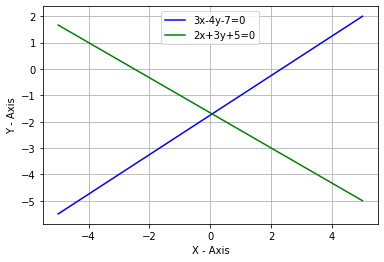
\includegraphics[width = \columnwidth]{./solutions/13/9/Lines.png}
\caption{Pair of Straight Lines}
\label{fig:solutions/13/9my_label}
\end{figure}


\item Find the value of k so that following equation may represent pairs of straight lines,
\begin{align}
kxy-8x+9y-12 = 0
\label{eq:solutions/13/10/Q_eq}
\end{align}
\solution
The general equation of second degree is given by,
\begin{align}
ax^2 + 2bxy + cy^2 + 2dx +2ey +f = 0
\label{eq:solutions/13/10/main_eq}
\end{align}
In vector from the equation \eqref{eq:solutions/13/10/main_eq} canb be expressed as,
\begin{align}
\vec{x}^T\vec{V}\vec{x} + 2\vec{u}^T\vec{x} + f = 0 
\label{eq:solutions/13/10/line_vec}
\end{align}
where,
\begin{align}
\vec{V} = \vec{V}^T = \myvec{a&b\\b&c}
\label{eq:solutions/13/10/vec1}
\end{align}
\begin{align}
\vec{u} = \myvec{d\\e}
\label{eq:solutions/13/10/vec2}
\end{align}
Now, comparing equation \eqref{eq:solutions/13/10/main_eq} to \eqref{eq:solutions/13/10/Q_eq} we get, a = c = 0, b = $\brak{\frac{k}{2}}$, d = -4, e = $\brak{\frac{9}{2}}$, f = -12.  
Hence, substituting these values in equation \eqref{eq:solutions/13/10/vec1} and \eqref{eq:solutions/13/10/vec2} we get,
\begin{align}
\vec{V} = \vec{V}^T = \myvec{0&\frac{k}{2}\\\frac{k}{2}&0}
\end{align}
\begin{align}
\vec{u} = \myvec{-4\\\frac{9}{2}}
\end{align}
Now equation \eqref{eq:solutions/13/10/Q_eq} represents pair of straight lines if,
\begin{align}
\mydet{\vec{V}&\vec{u}\\\vec{u}^T&f} = 0
\end{align}
\begin{align}
\mydet{0&\frac{k}{2}&-4\\\frac{k}{2}&0&\frac{9}{2}\\-4&\frac{9}{2}&-12} = 0
\end{align}
\begin{align}
\implies k =0 , k = 6 
\label{eq:solutions/13/10/k}
\end{align}
Substituting \eqref{eq:solutions/13/10/k} in \eqref{eq:solutions/13/10/Q_eq} we get,
\begin{align}
6xy-8x+9y-12 = 0
\end{align}
\begin{align}
-8x+9y-12 = 0
\end{align}
Hence value of k = 6 represents pair of straight lines.
Also it can be verified that the pair of lines intersect as,
\begin{align}
\mydet{\vec{V}} = \mydet{0&3\\3&0} <0 
\end{align} 
Let the pair of straight lines is given by,
\begin{align}
\vec{n_1}^T\vec{x} = c1
\label{eq:solutions/13/10/e1}
\end{align}
\begin{align}
\vec{n_2}^T\vec{x} = c2
\label{eq:solutions/13/10/e2}
\end{align}
Now equating the product of equation \eqref{eq:solutions/13/10/e1} and \eqref{eq:solutions/13/10/e2} with \eqref{eq:solutions/13/10/line_vec} we get,
\begin{align}
(\vec{n_1}^T\vec{x} - c1)(\vec{n_2}^T\vec{x} - c2) = \\\vec{x}^T\myvec{0&3\\3&0}\vec{x} + 2\myvec{-4& \frac{9}{2}}\vec{x} - 12 
\end{align}
\begin{align}
\implies n_1 * n_2 = \{0,6,0\}
\label{eq:solutions/13/10/verify}
\end{align}
\begin{align}
c_1n_1+c_2n_2 = \myvec{8\\-9}
\label{eq:solutions/13/10/sub1}
\end{align}
\begin{align}
c_1c_2 = -12.
\end{align}
Now the slopes of line is given by roots of polynomial,
\begin{align}
cm^2 + 2bm + a = 0
\end{align} 
\begin{align}
\implies 2bm = 0
\end{align}
\begin{align}
\implies m = 0
\end{align}
Also
\begin{align}
m_i = \frac{-b\pm\sqrt{-|V|}}{c} 
\end{align}
\begin{align}
\implies m_i = \frac{-0\pm\sqrt{9}}{0} 
\end{align}
\begin{align}
\therefore m_1 = 0
\end{align}
\begin{align}
 m_2 = \infty
\end{align}
The normal vector to the two lines is given by,
\begin{align}
n_i = k_i\myvec{-m_i\\1}
\end{align}
\begin{align}
\implies n_1 = k_1\myvec{0\\1}
\end{align}\\
\begin{align}
n_2 = k_2\myvec{1\\0}
\end{align}
Also,
\begin{align}
k_1k_2 = 6
\end{align}
Let $k_1$ = 2 and $k_2$ =3
\begin{align}
\implies n_1 = \myvec{0\\2}
\label{eq:solutions/13/10/n1}
\end{align}
\begin{align}
n_2 = \myvec{3\\0}
\label{eq:solutions/13/10/n2}
\end{align}
We verify obtained $n_1$ and $n_2$ using Toeplitz matrix,
\begin{align}
n_1*n_2 = \myvec{0&0\\2 &0\\0&2}\myvec{2\\0}\myvec{3\\0} = \myvec{0\\6\\0}
\label{eq:solutions/13/10/verify1}
\end{align}
Hence \eqref{eq:solutions/13/10/verify} and \eqref{eq:solutions/13/10/verify1} are same. Hence verified. 

Now substituting it in \eqref{eq:solutions/13/10/sub1} we get,
\begin{align}
c_2\myvec{0\\2}+c_1\myvec{3\\0} = \myvec{8\\-9}
\end{align}

Solve using Row reduction Technique we get,
\begin{align}
\implies\myvec{3&0&8\\0&2&-9} 
\end{align}

\begin{align}
\xleftrightarrow[]{R_1\leftarrow R_1/3}\myvec{1&0&8/3\\0&2&-9}
\end{align}
\begin{align}
\xleftrightarrow[]{R_2\leftarrow R_2/2}\myvec{1&0&8/3\\0&1&-9/2}
\end{align}
\begin{align}
\implies c_1 = \frac{8}{3}
\end{align}
\begin{align}
c_2 = \frac{-9}{2}
\end{align}
\begin{figure}[ht!]
\centering
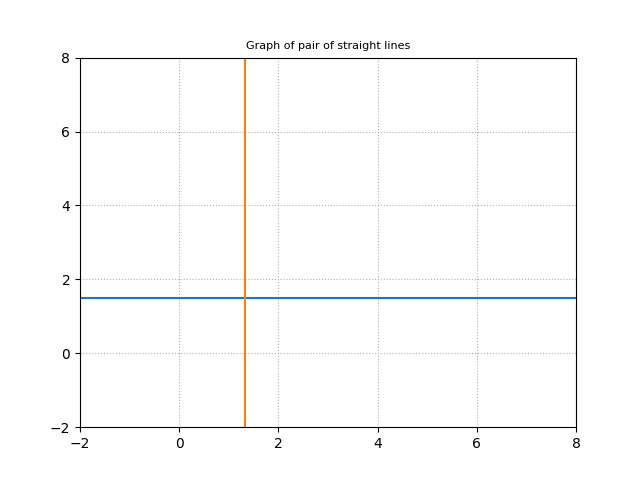
\includegraphics[width=\columnwidth]{./solutions/13/10/Figure_1.png}
\caption{Intersection of 2 lines}
\label{eq:solutions/13/10/Figure_1}
\end{figure}
substituting the values of $c_1$, $c_2$ and equation \eqref{eq:solutions/13/10/n1} and \eqref{eq:solutions/13/10/n2} to equation \eqref{eq:solutions/13/10/e1} and \eqref{eq:solutions/13/10/e2} we get equation of two straight lines.
\begin{align}
\implies \myvec{0&2}\vec{x} = \frac{8}{3}
\end{align}
\begin{align}
\myvec{3&0}\vec{x} = \frac{-9}{2}
\end{align}
Hence the equation of pair of straight lines are,
\begin{align}
\brak{\myvec{0&2}\vec{x}-\frac{8}{3}}\brak{\myvec{3&0}\vec{x} - \frac{-9}{2}} = 0
\label{eq:solutions/13/10/pair}
\end{align}
Hence, Plot of the equation \eqref{eq:solutions/13/10/pair} is shown in Figure.\ref{eq:solutions/13/10/Figure_1}
Now for value of k = 0 does not represent pair of straight lines.as,
\begin{align}
\mydet{\vec{V}} = \mydet{0&0\\0&0} \nless0 
\end{align} 
Hence, Plot of the equation $\myvec{-8&9}\vec{x} = 12$ is shown in figure \ref{eq:solutions/13/10/Figure_2},
\begin{figure}[ht!]
\centering
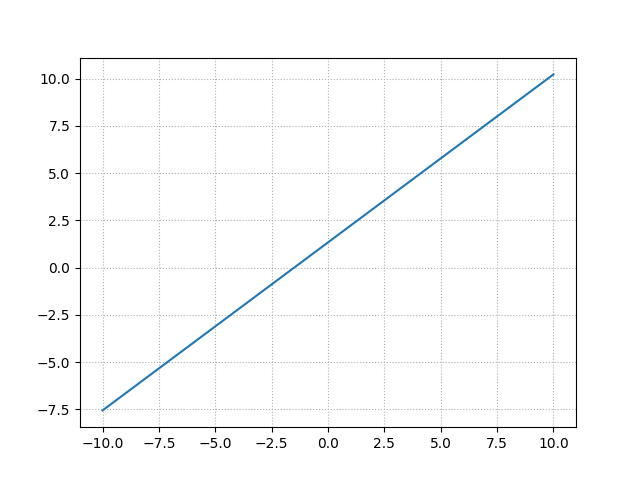
\includegraphics[width=\columnwidth]{./solutions/13/10/Figure_2.png}
\caption{Intersection of 2 lines}
\label{eq:solutions/13/10/Figure_2}
\end{figure}


\item Find the value of k such that 
\begin{align}
x^{2}+ \frac{10}{3}(xy)+y^2 -5x -7y + k =0 \label{eq:solutions/13/11eq5}
\end{align}
 represent pairs of straight lines.
\\
\solution
From  \eqref{eq:solutions/13/11eq5},
\begin{align}
	\vec{V} = \myvec{1& \frac{5}{3} \\ \frac{5}{3} & 1}\label{myeq:solutions/13/11/}\\
	\vec{u}^T = \myvec{\frac{-5}{2} & \frac{-7}{2}}\label{df:solutions/13/11/}
\end{align}
and
\begin{align}\label{eq:solutions/13/11/dett}
\mydet{1& \frac{5}{3} & \frac{-5}{2} \\ \frac{5}{3} & 1 & \frac{-7}{2} \\ \frac{-5}{2} & \frac{-7}{2} & k} = 0 \\
\implies \brak{k - \brak{\frac{49}{4}}}-\frac{5}{3}\brak{\frac{5}{3}k - \frac{35}{4}} \nonumber\\
-
\frac{5}{2} \brak{\frac{-35}{6}+\frac{5}{2}} = 0\\
\implies \frac{64}k{36} - \frac{128}{12} = 0\\
\implies \boxed{k = 6} \label{eq:solutions/13/11result}
\end{align}
Substituting \eqref{eq:solutions/13/11result} in \eqref{eq:solutions/13/11eq5}, we get
\begin{align}
	x^{2}+ \frac{10}{3}(xy)+y^2 -5x -7y + 6 =0  \label{eq:solutions/13/11reseq}
\end{align}
Hence value of k=6 represents pair of straight lines.
Substituting value of k =6 in \eqref{eq:solutions/13/11/dett}
\begin{align}
\delta&=\begin{array}{|ccc|}
1 &\frac{5}{3}& \frac{-5}{2}\\\frac{5}{3} & 1 & \frac{-7}{2}\\ \frac{-5}{2} & \frac{-7}{2} & 6
\end{array}&
\intertext{Simplyfying  the above determinant , we get}
\delta&=0
\end{align}
%Since equation \eqref{eq:solutions/13/11det1} is satisfied, we could say that the given equation 
\eqref{eq:solutions/13/11reseq} represents two straight lines
\begin{align}
    \det(V)&=\begin{array}{|cc|}
1&\frac{5}{3}\\\frac{5}{3} & 1
\end{array}<0
\end{align}
Since $\det(V)<0$  lines would intersect each other
\begin{figure}[h]
    \centering
    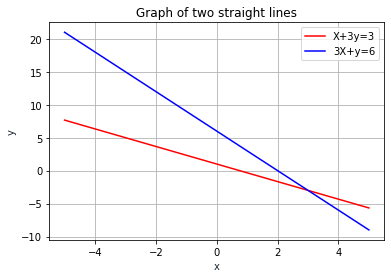
\includegraphics[width=\columnwidth]{./solutions/13/11/assignment5.png}
    \caption{Pair of straight lines}
    \label{Fig:solutions/13/11/1}
\end{figure}
%pair of straight lines in vector form is :
%\begin{align}
%    \vec{n_1}^T\vec{x}&=c_1\label{eq:solutions/13/11/m1}\\
%    \vec{n_2}^T\vec{x}&=c_2\label{eq:solutions/13/11/m2}
%\end{align}
%Equating their product with \eqref{eq:solutions/13/11eq4}
%\begin{align}
%(\vec{n_1}^T\vec{x}-c_1)(\vec{n_2}^T\vec{x}-c_2) &=\vec{x}^T\myvec{1 & \frac{5}{3} \\\frac{5}{3} & 1}\vec{x}\notag\\
%+2\myvec{\frac{-5}{2} & \frac{-7}{2}}\vec{x}+6\label{eq:solutions/13/11/86}
%\end{align}
\begin{align}
    \vec{n_1}*\vec{n_2}&=\{1,\frac{10}{3},1\}\label{eq:solutions/13/11/conv}\\
    c_2\vec{n_1}+c_1\vec{n_2}&=-2\myvec{\frac{-5}{2}\\\frac{-7}{2}}\label{eq:solutions/13/11/eq98}\\
    c_1c_2&=6
\end{align}
The slopes of the lines are given by the roots of the polynomial 
\begin{align}
    &cm^2+2bm+a=0\label{eq:solutions/13/11/e}\\
    \implies m_i&=\frac{-b\pm{\sqrt{-\det(V)}}}{c}\\
    \vec{n_i}&=k\myvec{-m_i\\1}
\end{align}
Substituting  in above equations \eqref{eq:solutions/13/11/e} we get,
\begin{align}
    &m^2+\frac{10}{3}m+1=0\\
    &\implies m_i=\frac{\frac{-10}{3}\pm{\sqrt{-(\frac{-16}{9})}}}{1}\label{eq:solutions/13/11/eq12}
\end{align}
Solving equation \eqref{eq:solutions/13/11/eq12} we have ,
\begin{align}
    m_1&=\frac{-1}{3}\\
    m_2&=-3\\
    \vec{n_1}&=k_1\myvec{\frac{1}{3}\\1}\label{eq:solutions/13/11/n1}\\
    \vec{n_2}&=k_2\myvec{{3}\\1}\label{eq:solutions/13/11/n2}
\end{align}
Substituting equations \eqref{eq:solutions/13/11/n1}, \eqref{eq:solutions/13/11/n2} in equation \eqref{eq:solutions/13/11/conv} we get 
\begin{align}
    k_1k_2&=1
\end{align}
Possible combination of ($k_1,k_2$) is (1,1)
Lets assume $k_1=1$, $k_2=1$, we get 
\begin{align}
    \vec{n_1}&=\myvec{\frac{1}{3} \\1}\label{eq:solutions/13/11/n11}\\
    \vec{n_2}&=\myvec{3\\1}\label{eq:solutions/13/11/n22}
\end{align}
we have:
\begin{align}
\vec{n_1}\ast \vec{n_2} = \myvec{a\\2b\\c} \label{eq:solutions/13/11conv1}
\end{align}
Convolution of $\vec{n_1}$ and $\vec{n_2}$ can be done by converting  $\vec{n_1}$ into a teoplitz matrix and multiplying with $\vec{n_2}$\\
From equation \eqref{eq:solutions/13/11/n11} and \eqref{eq:solutions/13/11/n22}
\begin{align}
    \vec{n_1}=\myvec{\frac{1}{3}&0\\1&\frac{1}{3}\\0&1}
    \vec{n_2}=\myvec{3\\ 1}\label{eq:solutions/13/11conv2}\\
\implies \myvec{\frac{1}{3}&0\\1&\frac{1}{3}\\0&1}\myvec{3\\ 1} = \myvec{1\\\frac{10}{3}\\1} = \myvec{a\\2b\\c}\label{eq:solutions/13/11conv3}
\end{align}
$c_1$ and $c_2$ can be obtained as,
\begin{align}
\myvec{\vec{n_1} & \vec{n_2}}\myvec{c_2\\c_1}&=-2\vec{u}\\
\myvec{\vec{n_1} & \vec{n_2}}\myvec{c_2\\c_1}&=-2\myvec{\frac{-5}{2}\\\frac{-7}{2}}
\label{eq:solutions/13/11aug1}
\end{align}
Substituting \eqref{eq:solutions/13/11/n11} and \eqref{eq:solutions/13/11/n22} in \eqref{eq:solutions/13/11aug1}, the augmented matrix is,
\begin{align}
\myvec{\frac{1}{3} & 3& 5 \\ 1 & 1 & 7}
\xleftrightarrow[]{R_1 \leftarrow 3\times R_1}
\myvec{1 & 9&15\\ 1 & 1 & 7}
\end{align}
\begin{align}
\myvec{1 & 9&15\\ 1 & 1 & 7}
\xleftrightarrow[]{R_2 \leftarrow R_2- R_1}
\myvec{1 & 9&15\\ 0 & -8 & -8}
\end{align}
\begin{align}
\myvec{1 & 9&15\\ 0 & -8 & -8}
\xleftrightarrow[]{R_2 \leftarrow R_2\div -8}
\myvec{1 & 9&15\\ 0 & 1 & 1}
\end{align}
\begin{align}
\myvec{1 & 9&15\\ 0 & 1 & 1}
\xleftrightarrow[]{R_1 \leftarrow R_1-9\times R_2}
\myvec{1 & 0&6\\ 0 & 1&1 }
\end{align}
From above  we get 
\begin{align}
    c_1&=1\\
    c_2&=6
\end{align}
Hence pair of straight lines  are
%from  \eqref{eq:solutions/13/11/m1}, \eqref{eq:solutions/13/11/m2} in vector form
\begin{align}
    \myvec{\frac{1}{3}& 1}\vec{x}&=1\\
    \myvec{3 & 1}\vec{x}&=6
\end{align}

   

\item Prove that the equation
\begin{align}
	12x^2 + 7xy -10y^2 +13x +45y -35 =0 
\end{align}
represents two straight lines and find the angle between the lines.
\\
\solution
The above equation can be expressed as
\begin{align}
        \vec{x}^{T}\vec{Vx} + 2\vec{u}^{T}\vec{x} + f=0   \label{eq:solutions/13/12/eq2}
\end{align}
where
\begin{align}
	\vec{V}=\vec{V}^T &= \myvec{12 & \frac{7}{2} \\ \frac{7}{2} & -10} \\
	\vec{u} &= \myvec{\frac{13}{2} \\ \frac{45}{2}} \\
	 f=-35
\end{align}	
	(\ref{eq:solutions/13/12/eq2}) represents a pair of straight lines if
\begin{align}
	&\mydet{\vec{V} & \vec{u} \\ \vec{u}^T & f} = 0     \label{eq:solutions/13/12/eq5} \\
	\mydet{\vec{V} & \vec{u} \\ \vec{u}^T & f} 
		&= \mydet{12 & \frac{7}{2}  & \frac{13}{2} \\ 
	        \frac{7}{2} & -10 & \frac{45}{2}     \\
	       \frac{13}{2} & \frac{45}{2} & -35 }  \\
	       		\nonumber \\
	\implies \ 12\mydet{-10 & \frac{45}{2} \\ \frac{45}{2} & -35} 
		& -\frac{7}{2}\mydet{\frac{7}{2} & \frac{45}{2} \\ \frac{13}{2} & -35} 
		+\frac{13}{2}\mydet{\frac{7}{2} & -10 \\ \frac{13}{2} & \frac{45}{2}} = 0 \label{eq:solutions/13/12/eq10}\\
\end{align}
The lines intercept if
\begin{align}
        \mydet{\vec{V}} < 0 \\
 	\mydet{\vec{V}}=-\frac{529}{4} < 0 \label{eq:solutions/13/12/eq11}
\end{align}
From (\ref{eq:solutions/13/12/eq10}) and (\ref{eq:solutions/13/12/eq11}) it can be concluded that the given equation represents a pair of intersecting lines.
Let the equations of lines be
\begin{align}
	\vec{n_1}^T \vec{x}=c_1 \\
	\vec{n_2}^T \vec{x}=c_2 
\end{align}
Since (\ref{eq:solutions/13/12/eq2}) represents a pair of straight lines it must satisfy
\begin{align}
	(\vec{n_1}^T \vec{x} - c_1)(\vec{n_1}^T \vec{x} - c_1) =
        \vec{x}^{T}\vec{Vx} + 2\vec{u}^{T}\vec{x} + f=0
\end{align}
where
\begin{align}
	\vec{n_1}*\vec{n_2}=\myvec{a\\2b\\c}=\myvec{12\\7\\-10} \label{eq:solutions/13/12/eq6} \\ 
	c_2\vec{n_1}+c_1\vec{n_2}=-2\vec{u} \label{eq:solutions/13/12/eq9}\\
	c_1c_2=f
\end{align}
Slopes of the lines can be obtained by solving 
\begin{align}
	cm^2+2bm+a=0 \\
	-10m^2+7m+12=0 \\
	\implies m_1 = \frac{-4}{5}, m_2 = \frac{3}{2}
\end{align}
The normal vectors can be expressed in terms of corresponding slopes of lines as
\begin{align}
	\vec{n}=k\myvec{-m\\1} \\
	\implies
	\vec{n_1}=k_1\myvec{\frac{4}{5} \\ 1}  \label{eq:solutions/13/12/eq7} \\
	\vec{n_2}=k_2\myvec{-\frac{3}{2} \\ 1}  \label{eq:solutions/13/12/eq8}
\end{align}
Substituing (\ref{eq:solutions/13/12/eq7}) and (\ref{eq:solutions/13/12/eq8}) in (\ref{eq:solutions/13/12/eq6}) we get
\begin{align}
	k_1k_2=-10
\end{align}
Assuming $ k_1=5$ and $k_2 =-2$
\begin{align}
	\vec{n_1}=\myvec{4\\5}, \vec{n_2}=\myvec{3\\-2}
\end{align}
Verification using Toeplitz matrix
\begin{align}
\vec{n_1}*\vec{n_2}=\myvec{4 & 0 \\ 5 & 4 \\0 & 5}\myvec{3\\-2}=\myvec{12\\7\\-10}
\end{align}
From (\ref{eq:solutions/13/12/eq9}) we have
\begin{align}
	c_2\myvec{4\\5}+c_1\myvec{3\\-2}=\myvec{-13\\-45}
\end{align}
Solving the augmented matrix
\begin{align}
	\myvec{4 & 3 & -13 \\ 5 & -2 & -45}
	\xleftrightarrow[]{R_2 \leftarrow 4R_2-5R_1}
	\myvec{4 & 3 & -13 \\ 0 & -23 & -115}\\
	\xleftrightarrow[]{R_2 \leftarrow -\frac{R_2}{23}}
        \myvec{4 & 3 & -13 \\ 0 & 1 & 5}
        \xleftrightarrow[]{R_1 \leftarrow R_1-3R_2}
	\myvec{4 & 0 & -28 \\ 0 & 1 & 5}\\
	\xleftrightarrow[]{R_1 \leftarrow \frac{R_1}{4}}
        \myvec{1 & 0 & -7 \\ 0 & 1 & 5} \\
	\implies \quad c_1 =-7, \ c_2 =5
\end{align}
Thus the equation of lines are
\begin{align}
	\myvec{4 & 5}\vec{x} = 5 \\
	\myvec{3 & -2}\vec{x} = -7 
\end{align}
The angle between the lines can be expressed interms of normal vectors 
\begin{align}
	\vec{n_1}=\myvec{4\\5} , \quad \vec{n_2}=\myvec{3\\-2}
\end{align}
as
\begin{align}
	\cos\theta=\frac{\vec{n_1}^T\vec{n_2}}{\norm{\vec{n_1}}\norm{\vec{n_2}}} \\
				\nonumber \\
	\implies \quad \theta=\cos^{-1}({\frac{2}{\sqrt{533}}}) = \tan^{-1}(\frac{23}{2})
\end{align}
\begin{figure}[!h]
	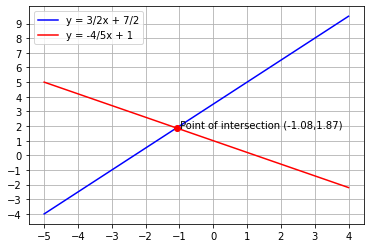
\includegraphics[width=\columnwidth]{./solutions/13/12/lines.png}
	\caption{} \label{eq:solutions/13/12/linefig1}
\end{figure}


\item Find the value of k so that the following equation may represent the pair of staright lines:
\begin{align}
	2x^2+ xy -y^2 + kx + 6y - 9 = 0 \label{eq:solutions/13/13/1} 
\end{align}

\solution
We need to find the value of k for which \eqref{eq:solutions/13/13/1} represents a pair of straight lines.

Converting \eqref{eq:solutions/13/13/1} into vector form, we get
\begin{align}
	\vec{x}^T\myvec{2 & 1/2 \\ 1/2 & -1}\vec{x}+2\myvec{k/2 \\ 3}\vec{x}-9=0 \label{eq:solutions/13/13/2}
\end{align} 
Here, we have
\begin{align}
& \vec{V} = \vec{V}^T = \myvec{2 & 1/2 \\ 1/2 & -1} \\
& \vec{u} = \myvec{k/2 \\ 3} \\
& f = -9
\end{align}
The above represents a pair of straight lines if
\begin{align}
	\begin{array}{|cc|}
		\vec{V} & \vec{u}\\\vec{u}^T & f
	\end{array}&=0\label{eq:solutions/13/13/3}
\end{align}
Since \eqref{eq:solutions/13/13/1} represents a pair of straight lines, then by \eqref{eq:solutions/13/13/3}, we have
\begin{align}
	\begin{array}{|ccc|}
		2 & 1/2 & k/2 \\ 1/2 & -1 & 3  \\ k/2 & 3 & -9 
	\end{array}&=0
\end{align}
By solving, above determinant we get
\begin{align}
& 2(9-9) + \frac{-1}{2}(\frac{-9}{2} + \frac{-3k}{2}) + \frac{k}{2}(\frac{3}{2} + \frac{k}{2})  = 0\\
& \frac{(9+3k)}{4} + \frac{k(3+k)}{4}  = 0 \\
& k^2 + 6k + 9 =0 \\
& (k+3)^2 = 0 \\
& k = -3 \label{eq:solutions/13/13/4}
\end{align}
Hence by \eqref{eq:solutions/13/13/4}, we have
\begin{align}
   2x^2+ xy -y^2 - 3x + 6y - 9 &= 0
\end{align} 
represents family of straight lines for $k=-3$.


To find the staright lines, we write each of thrm in their vector form as
\begin{align}
	& \vec{n_1}^T\vec{x} =c_1 \\
	& \vec{n_2}^T\vec{x} =c_2 
\end{align} 
Equating the product of above with \eqref{eq:solutions/13/13/2}, we have
\begin{multline}
 \brak{\vec{n_1}^T\vec{x}-c_1}\brak{\vec{n_2}^T\vec{x}-c_2} = \\ 
\vec{x}^T\myvec{2 & 1/2 \\ 1/2 & -1}\vec{x}+2\myvec{k/2 \\ 3}\vec{x}-9
\end{multline}
\begin{align}
\implies & \vec{n_1}*\vec{n_2} = \myvec{2 \\ 1 \\ -1}\label{eq:solutions/13/13/5} \\
& c_2\vec{n_1} + c_1\vec{n_1} =-2\myvec{-3/2 \\ 3}\label{eq:solutions/13/13/6} \\
& c_1c_2 = -9 \label{eq:solutions/13/13/7}
\end{align}
Here, the slope of these lines are given by the roots of the polynomial
\begin{align}
-& m^2 + m + 2 = 0 \\ 
 & m^2 - m - 2 = 0 \\
 & m = \frac{1 \pm \sqrt{1+8}}{2} \\
 & m_1 = \frac{1+3}{2} = 2 \\
 & m_2 = \frac{1-3}{2} = -1 \\
 & n_1 = k_1\myvec{-2 \\ 1}\label{eq:solutions/13/13/8} \\
 & n_2 = k_2\myvec{1 \\ 1}\label{eq:solutions/13/13/9}
\end{align}
Substituing \eqref{eq:solutions/13/13/8} and \eqref{eq:solutions/13/13/9} in \eqref{eq:solutions/13/13/5}, we get
\begin{align}
	k_1k_2 = -1
\end{align}
Taking $k_1=-1$ and $k_2=1$, we get
\begin{align}
	& n_1 = \myvec{2 \\ -1} \\
	& n_2 = \myvec{1 \\ 1}
\end{align}
Substituting in \eqref{eq:solutions/13/13/6} for  above values of$n_1$ and $n_2$
\begin{align}
& \myvec{ n_1 n_2} \myvec{c_2 \\ c_1} \quad= \myvec{3\\-6} \\
& \myvec{2 &1 \\ -1 &1} \myvec{c_2 \\ c_1} = \myvec{3\\-6}\label{eq:solutions/13/13/10}
\end{align}
Solving \eqref{eq:solutions/13/13/10},
\begin{multline}
\myvec{2 &1 \\ -1 &1} \myvec{c_2 \\ c_1} = \myvec{3\\-6} \xLeftrightarrow[]{r_2 = r_2 + 2r_1} \\
\myvec{2 &1 \\ 0 &3} \myvec{c_2 \\ c_1} = \myvec{3\\-9}
\end{multline}
\begin{multline}
	\myvec{2 &1 \\ 0 &3} \myvec{c_2 \\ c_1} = \myvec{3\\-9} \xLeftrightarrow[]{r_2 = r_2/3} \\
	\myvec{2 &1 \\ 0 &1} \myvec{c_2 \\ c_1} = \myvec{3\\-3}
\end{multline}
\begin{multline}
	\myvec{2 &1 \\ 0 &1} \myvec{c_2 \\ c_1} = \myvec{3\\-3} \xLeftrightarrow[]{r_1 = r_1-r_2} \\
	\myvec{2 &0 \\ 0 &1} \myvec{c_2 \\ c_1} = \myvec{6\\-3}
\end{multline}
Hence, we found out
\begin{align}
	&c_1 = -3 \\
	&c_2 = 3
\end{align}
Thus, pair of staright lines are
\begin{align}
& \myvec{2 &-1}\vec{x} = -3 \\
& \myvec{1 &1}\vec{x} = 3 
\end{align}
where
\begin{align}
\vec{x} = \myvec{x \\ y}	
\end{align}
The plot of above is shown below 
\begin{figure}[!htb]
	
	\centering
	
	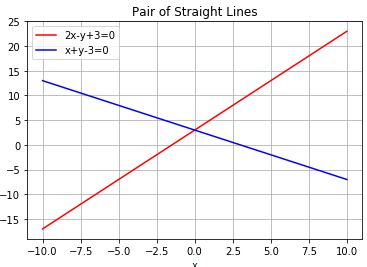
\includegraphics[width=\columnwidth]{./solutions/13/13/Latex/assignment4fig.jpg}
	
	\caption{Pair of Straight Lines}
	
	\label{eq:solutions/13/13/fig:1}
	
\end{figure}


%
\item Prove that the equation $12x^2+7xy-10y^2+13x+45y-35=0$ represents two straight lines and find the angle between them. 
\\
\solution
The general second order equation is given by ,
\begin{align}
ax^2+2bxy+cy^2+2dx+2ey+f&=0\label{eq:solutions/13/ex1/eq1}
\end{align}
Given,
\begin{align}
    12x^2+7xy-10y^2+13x+45y-35&=0 \label{eq:solutions/13/ex1/eqgiven}
\end{align}
The above equation can be expressed as
\begin{align}
        \vec{x}^{T}\vec{Vx} + 2\vec{u}^{T}\vec{x} + f=0   \label{eq:solutions/13/ex1/eq:solutions/eq2}
\end{align}
where
\begin{align}
	\vec{V}=\vec{V}^T &= \myvec{12 & \frac{7}{2} \\ \frac{7}{2} & -10} \\
	\vec{u} &= \myvec{\frac{13}{2} \\ \frac{45}{2}} \\
	 f=-35
\end{align}	
	(\ref{eq:solutions/13/ex1/eq:solutions/eq2}) represents a pair of straight lines if
\begin{align}
	&\mydet{\vec{V} & \vec{u} \\ \vec{u}^T & f} = 0     \label{eq:solutions/13/ex1/eq:solutions/eq5} \\
	\mydet{\vec{V} & \vec{u} \\ \vec{u}^T & f} 
		&= \mydet{12 & \frac{7}{2}  & \frac{13}{2} \\ 
	        \frac{7}{2} & -10 & \frac{45}{2}     \\
	       \frac{13}{2} & \frac{45}{2} & -35 }  \\
	       		\nonumber \\
	\implies \ 12\mydet{-10 & \frac{45}{2} \\ \frac{45}{2} & -35} 
		& -\frac{7}{2}\mydet{\frac{7}{2} & \frac{45}{2} \\ \frac{13}{2} & -35} 
		+\frac{13}{2}\mydet{\frac{7}{2} & -10 \\ \frac{13}{2} & \frac{45}{2}} = 0 \label{eq:solutions/13/ex1/eq:solutions/eq10}
\end{align}
The lines intercept if
\begin{align}
        \mydet{\vec{V}} < 0 \\
 	\mydet{\vec{V}}=-\frac{529}{4} < 0 \label{eq:solutions/13/ex1/eq:solutions/eq11}
\end{align}
\renewcommand{\thefigure}{1}
From (\ref{eq:solutions/13/ex1/eq:solutions/eq10}) and (\ref{eq:solutions/13/ex1/eq:solutions/eq11}) it can be concluded that the given equation represents a pair of intersecting lines.\\
Let $(\alpha,\beta)$ be their point of intersection, then
\begin{align}
	\label{eq:solutions/13/ex1/eq16}\myvec{ 12 & \frac{7}{2}\\\frac{7}{2} & -10}\myvec{\alpha \\ \beta} = \myvec{\frac{-13}{2} \\ -\frac{45}{2}} \\
	\label{eq:solutions/13/ex1/eq17}\implies \myvec{\alpha \\ \beta} = \myvec{-1 \\ 2}
\end{align}
\begin{equation}
	\text{From \textit{Spectral theorem, }}\vec{V} = \vec{P}\vec{D}\vec{P}^T
\end{equation}
\begin{align}
	\label{eq:solutions/13/ex1/eq18}\vec{V} &= \myvec{ 12 & \frac{7}{2}\\ \frac{7}{2} & -10}\\
	\label{eq:solutions/13/ex1/eq19}\vec{P} &= \myvec{\frac{-\sqrt{533} - 22}{2} & \frac{-22 + \sqrt{533}}{2}\\ 1 & 1}\\
	\label{eq:solutions/13/ex1/eq20}\vec{D} &= \myvec{1 + \frac{\sqrt{533}}{2} & 0\\ 0 & 1 - \frac{\sqrt{533}}{2}}
\end{align}
Using \textit{Spectral decomposition} of matrix we can express equation as
\begin{align}
	\label{eq:solutions/13/ex1/eq14}u_1(x-\alpha) + u_2(y-\beta) &= \pm \sqrt{-\frac{\lambda_2}{\lambda_1}}(v_1(x-\alpha) + v_2(y-\beta))
\end{align}
Substituting values in above equation we get;
\begin{multline}\label{eq:solutions/13/ex1/eq21}
	\frac{\sqrt{533}-22}{2}(x+1) + (y-2) \\= \pm \sqrt{-\frac{1 - \frac{\sqrt{533}}{2}}{1 + \frac{\sqrt{533}}{2}}}\left(\frac{-22 -\sqrt{533}}{2}(x+1) + (y-2)\right)
\end{multline}
Simplifying \eqref{eq:solutions/13/ex1/eq21},
\begin{align}
	\label{eq:solutions/13/ex1/eq22}3x -2y + 7 = 0 \text{ and } 4x + 5y -5 = 0\\
	\implies (3x - 2y + 7)(4x + 5y - 5) = 0
\end{align}
Thus the equation of lines are
\begin{align}
	\myvec{4 & 5}\vec{x} = 5 \\
	\myvec{3 & -2}\vec{x} = -7 
\end{align}
\begin{figure}[h]
    \centering
    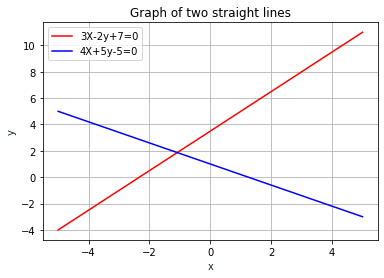
\includegraphics[width=\columnwidth]{./solutions/13/ex1/Figure.png}
    \caption{Pair of straight lines}
    \label{eq:solutions/13/ex1/Fig :1}
\end{figure}
{Angle between the straight lines: }
The angle between the lines can be expressed in terms of normal vectors 
\begin{align}
	\vec{n_1}=\myvec{4\\5} , \quad \vec{n_2}=\myvec{3\\-2}
\end{align}
\begin{align}
	\cos\theta=\frac{\vec{n_1}^T\vec{n_2}}{\norm{\vec{n_1}}\norm{\vec{n_2}}} \\
				\nonumber \\
	\implies \quad \theta=\cos^{-1}({\frac{2}{\sqrt{533}}}) = \tan^{-1}(\frac{23}{2})
\end{align}

\item Find the value of $h$ so that the equation 
\begin{align}
6x^2+2hxy+12y^2+22x+31y+20=0
\label{eq:solutions/13/ex2/question}
\end{align}
 may represent two straight lines.
\\
\solution
The general equation second degree is given by
\begin{equation}\label{eq:solutions/13/ex2/eq1}
	ax^2 + 2bxy + cy^2 + 2dx + 2ey + f = 0
\end{equation}
\eqref{eq:solutions/13/ex2/eq1} represents pair of straight lines if
\begin{equation}\label{eq:solutions/13/ex2/eq2}
	\mydet{ a & h & d\\
			h & c & e\\
			d & e & f} = 0
\end{equation}
From \eqref{eq:solutions/13/ex2/eq2}, given equation represents pair of straight lines if 
\begin{equation}\label{eq:solutions/13/ex2/eq3}
	\mydet{ 6 & h & 11\\
			h & 12 & \frac{31}{2}\\
			11 & \frac{31}{2} & 20} = 0
\end{equation}
\begin{equation}\label{eq:solutions/13/ex2/eq4}
	\implies h = \frac{17}{2} \text{ or } h = \frac{171}{20}
\end{equation}
Verify  \eqref{eq:solutions/13/ex2/eq4} using python code from
\begin{lstlisting}
https://github.com/shreeprasadbhat/matrix-theory/tree/master/assignment5/codes/solve_determinant.py
\end{lstlisting}
The general equation second degree is given by
\begin{equation}\label{eq:solutions/13/ex2/eq5}
	ax^2 + 2bxy + cy^2 + 2dx + 2ey + f = 0
\end{equation}
Let $(\alpha,\beta)$ be their point of intersection, then
\begin{equation}\label{eq:solutions/13/ex2/eq6}
	\myvec{ a & h\\ h & b}\myvec{\alpha \\ \beta} = \myvec{-d \\ -e}
\end{equation}
Under \textit{Affine transformation},
\begin{align}
	\vec{x} &= \vec{M}\vec{y} + c\\
	\myvec{x \\ y} &= \myvec{1 & 0 \\ 0 & 1} \myvec{X \\ Y} + \myvec{\alpha \\ \beta}\\
	\label{eq:solutions/13/ex2/eq7}\myvec{x \\ y} &= \myvec{X+\alpha \\ Y+\beta}
\end{align}
\eqref{eq:solutions/13/ex2/eq5} under transformation \eqref{eq:solutions/13/ex2/eq7} will become,
\begin{equation}\label{eq:solutions/13/ex2/eq8}
	aX^2 + 2bXY + cY^2 = 0
\end{equation}
\begin{equation}\label{eq:solutions/13/ex2/eq9}
	\myvec{X & Y} \myvec{a & h \\ h & b} \myvec{X \\ Y} = 0
\end{equation}
%\begin{equation}\label{eq:solutions/13/ex2/eq10}
%	\vec{X}^T\vec{V}\vec{X} = 0
%\end{equation}
\begin{equation}\label{eq:solutions/13/ex2/eq11}
	\myvec{X & Y} \myvec{u_1 & v_1 \\ u_2 & v_2} \myvec{\lambda_1 & 0\\ 0 & \lambda_2} \myvec{u_1 & u_2 \\ v_1 & v_2} \myvec{X \\ Y} = 0
\end{equation}
\begin{equation}\label{eq:solutions/13/ex2/eq12}
	\myvec{X^\prime & Y^\prime}  \myvec{\lambda_1 & 0\\ 0 & \lambda_2} \myvec{X^\prime \\ Y^\prime} = 0
\end{equation}
where $X^\prime = Xu_1 + Yu_2$ and $Y^\prime = Xv_1 + Yv_2$
\begin{equation}\label{eq:solutions/13/ex2/eq13}
	\implies \lambda_1 (X^\prime)^2 + \lambda_2 (Y^\prime)^2 = 0
\end{equation}
This is called \textit{Spectral decomposition} of matrix
\begin{align}
	X^\prime &= \pm \sqrt{-\frac{\lambda_2}{\lambda_1}}Y^\prime\\
	u_1X + u_2Y &= \pm \sqrt{-\frac{\lambda_2}{\lambda_1}}(v_1X + v_2Y)\\
	\label{eq:solutions/13/ex2/eq14}u_1(x-\alpha) + u_2(y-\beta) &= \pm \sqrt{-\frac{\lambda_2}{\lambda_1}}(v_1(x-\alpha) + v_2(y-\beta))
\end{align}
Given equation is
\begin{equation}\label{eq:solutions/13/ex2/eq15}
	6x^2 + 17xy + 12y^2 + 22x + 31y + 20 = 0
\end{equation}
Substituting in \eqref{eq:solutions/13/ex2/eq6}
\begin{align}
	\label{eq:solutions/13/ex2/eq16}\myvec{ 6 & \frac{17}{2}\\\frac{17}{2} & 12}\myvec{\alpha \\ \beta} = \myvec{-11 \\ -\frac{31}{2}} \\
	\label{eq:solutions/13/ex2/eq17}\implies \myvec{\alpha \\ \beta} = \myvec{1 \\ -2}
\end{align}
Verify  \eqref{eq:solutions/13/ex2/eq17} using python code from
\begin{lstlisting}
https://github.com/shreeprasadbhat/matrix-theory/tree/master/assignment5/codes/find_intersection.py
\end{lstlisting}
{Taking $h=\frac{17}{2}$}
\begin{align}
	\vec{V} &= \vec{P}\vec{D}\vec{P}^T\\
	\label{eq:solutions/13/ex2/eq18}\vec{V} &= \myvec{ 6 & \frac{17}{2}\\ \frac{17}{2} & 12}\\
	\label{eq:solutions/13/ex2/eq19}\vec{P} &= \myvec{\frac{-5\sqrt{13} - 6}{17} & \frac{-6 + 5\sqrt{13}}{17}\\ 1 & 1}\\
	\label{eq:solutions/13/ex2/eq20}\vec{D} &= \myvec{9 - \frac{5\sqrt{13}}{2} & 0\\ 0 & 9 + \frac{5\sqrt{13}}{2}}
\end{align}
Verify  \eqref{eq:solutions/13/ex2/eq19} and \eqref{eq:solutions/13/ex2/eq20} using python code from
\begin{lstlisting}
https://github.com/shreeprasadbhat/matrix-theory/tree/master/assignment5/codes/diagonalize1.py
\end{lstlisting}
Substituting \eqref{eq:solutions/13/ex2/eq17}, \eqref{eq:solutions/13/ex2/eq19} and \eqref{eq:solutions/13/ex2/eq20} in \eqref{eq:solutions/13/ex2/eq14},
\begin{multline}\label{eq:solutions/13/ex2/eq21}
	\frac{-5\sqrt{13} - 6}{17}(x+1) + (y-2) \\= \pm \sqrt{-\frac{9 + \frac{5\sqrt{13}}{2}}{9 - \frac{5\sqrt{13}}{2}}}\left(\frac{-6 + 5\sqrt{13}}{17}(x+1) + (y+2)\right)
\end{multline}
Simplifying \eqref{eq:solutions/13/ex2/eq21},
\begin{align}
	\label{eq:solutions/13/ex2/eq22}2x + 3y + 4 = 0 \text{ and } 3x + 4y + 5 = 0\\
	\implies (2x + 3y + 4)(3x + 4y + 5) = 0
\end{align}
Verify  \eqref{eq:solutions/13/ex2/eq22} using python code from
\begin{lstlisting}
https://github.com/shreeprasadbhat/matrix-theory/tree/master/assignment5/codes/calculate1.py
\end{lstlisting}

%\renewcommand{\thefigure}{\theenumi.\arabic*}
%\renewcommand{\thefigure}{\thesection.\arabic}
\begin{figure}[!ht]
	\centering
	\includegraphics[width=\columnwidth]{./solutions/13/ex2/fig/figure_1.png}
	\caption{Pair of straight lines $3x + 4y + 5 = 0$ and $2x + 3y + 4 = 0$}
	\label{eq:solutions/13/ex2/fig:figure1}
\end{figure}
{Taking $h=\frac{171}{20}$}
\begin{align}
	\vec{V} &= \vec{P}\vec{D}\vec{P}^T\\
	\vec{V} &= \myvec{ 6 & \frac{171}{2}\\ \frac{171}{2} & 12}\\
	\label{eq:solutions/13/ex2/eq23}\vec{P} &= \myvec{\frac{-\sqrt{3649} - 20}{57} & \frac{-20 + \sqrt{3649}}{57}}\\
	\label{eq:solutions/13/ex2/eq24}\vec{D} &= \myvec{9 - \frac{3\sqrt{3649}}{20} & 0\\ 0 & 9 + \frac{3\sqrt{3649}}{20}}
\end{align}
Verify  \eqref{eq:solutions/13/ex2/eq23} and \eqref{eq:solutions/13/ex2/eq24} using python code from
\begin{lstlisting}
https://github.com/shreeprasadbhat/matrix-theory/tree/master/assignment5/codes/diagonalize2.py
\end{lstlisting}
Substituting \eqref{eq:solutions/13/ex2/eq17},\eqref{eq:solutions/13/ex2/eq23} and \eqref{eq:solutions/13/ex2/eq24} in \eqref{eq:solutions/13/ex2/eq14}, 
\begin{multline}\label{eq:solutions/13/ex2/eq25}
	\frac{-\sqrt{3649} - 20}{57}(x+1) + (y-2) \\= \pm 
	\sqrt{-\frac{9 + \frac{3\sqrt{3649}}{20}}{9 - \frac{3\sqrt{3649}}{20}}}\\
	\left(\frac{-20 + \sqrt{3649}}{57}(x+1) + (y+2)\right)
\end{multline}
Simplifying \eqref{eq:solutions/13/ex2/eq24},
\begin{align}
	\label{eq:solutions/13/ex2/eq26}2x + 3y + 4 = 0 \text{ and } 3x + 4y + 5 = 0\\
	\label{eq:solutions/13/ex2/eq27}\implies (2x + 3y + 4)(3x + 4y + 5) = 0
\end{align}
Verify  \eqref{eq:solutions/13/ex2/eq25} using python code from
\begin{lstlisting}
https://github.com/shreeprasadbhat/matrix-theory/tree/master/assignment5/codes/calculate2.py
\end{lstlisting}
\begin{figure}[ht!]
	\centering
	\includegraphics[width=\columnwidth]{./solutions/13/ex2/fig/figure_2.png}
	\caption{Pair of straight lines $4x + 5y + \frac{20}{3} = 0$ and $5x + 8y + 10 = 0$}
	\label{eq:solutions/13/ex2/fig:figure2}
\end{figure}
%\renewcommand{\thefigure}{\theenumi}



\end{enumerate}




\section{General Equation. Tracing of Curves}
\subsection{40}
\renewcommand{\theequation}{\theenumi}
\renewcommand{\thefigure}{\theenumi}
\begin{enumerate}[label=\thesubsection.\arabic*.,ref=\thesubsection.\theenumi]
\numberwithin{equation}{enumi}
\numberwithin{figure}{enumi}
%
\item What conics do the following equation represent? When possible, find the centres and also their equations referred to the centre

\begin{align}
12x^2-23xy+10y^2-25x+26y=14\label{eq:solutions/40/1/ques}
\end{align}
\\
\solution
The given equation \eqref{eq:solutions/40/1/ques} can be expressed as 
\begin{align}
&\vec{x}^T\myvec{12 & \frac{-23}{2}\\\frac{-23}{2} & 10}\vec{x}+2\myvec{\frac{-25}{2} & 13}\vec{x}-14=0\label{eq:solutions/40/1/given}
\end{align}

where 
\begin{align}
\vec{V}&=\myvec{12 & \frac{-23}{2}\\\frac{-23}{2} & 10}\\
\vec{u}&=\myvec{\frac{-25}{2} \\ 13}\\
f&=-14
\end{align}

\begin{align}
    \det(\vec{V})&=\begin{array}{|cc|}
12 & \frac{-23}{2}\\\frac{-23}{2} & 10
\end{array}\\
\implies\det(\vec{V})&=\frac{-49}{4}\\
\implies\det(\vec{V})&<0
\end{align}

Since $\det(\vec{V})<0$ the given equation \eqref{eq:solutions/40/1/given} represents the hyperbola
The characteristic equation of $\vec{V}$ is obtained by evaluating the determinant 

\begin{align}
       \begin{array}{|c|}
V-\lambda\vec{I}
\end{array}&=0\\
   \begin{array}{|cc|}
12-\lambda & \frac{-23}{2} \\ \frac{-23}{2} & 10-\lambda
\end{array}&=0\\
\implies 4\lambda^2-88\lambda-49&=0\label{eq:solutions/40/1/eqroots}
\end{align}

The eigenvalues are the roots of equation \ref{eq:solutions/40/1/eqroots} is given by 
\begin{align}
    \lambda_1&=\frac{22+\sqrt{533}}{2}\label{eq:solutions/40/1/eqeig1}\\
    \lambda_2&=\frac{22-\sqrt{533}}{2}\label{eq:solutions/40/1/eqeig2}
\end{align}

The eigenvector $\vec{p}$ is defined as 
\begin{align}
    \vec{V}\vec{p}&=\lambda\vec{p}\\
    \implies (\vec{V}-\lambda\vec{I})\vec{p}&=0\label{eq:solutions/40/1/eqev}
\end{align}

For $\lambda_1=\frac{22-\sqrt{533}}{2}$ ,
\begin{align}
    (\vec{V}-\lambda_1\vec{I})=\myvec{\frac{\sqrt{553}+2}{2} & \frac{-23}{2} \\\frac{-23}{2} & \frac{\sqrt{533}-2}{2}}
\end{align}

By row reduction , 
\begin{align}
    &\myvec{\frac{\sqrt{533}+2}{2} & \frac{-23}{2} \\\frac{-23}{2} & \frac{\sqrt{533}-2}{2}}\\
    &\xleftrightarrow{R_1=\frac{R_1}{\frac{\sqrt{533}+2}{2}}}\myvec{1 & \frac{2-\sqrt{533}}{23} \\\frac{-23}{2} & \frac{\sqrt{533}-2}{2}}\\
    &\xleftrightarrow{R_2=R_2+\frac{23}{2}R_1}\myvec{1 & \frac{2-\sqrt{533}}{23} \\0 & 0}\label{eq:solutions/40/1/eqs1}
\end{align}

Subsituting equation \ref{eq:solutions/40/1/eqs1} in equation \ref{eq:solutions/40/1/eqev} we get
\begin{align}
        &\myvec{1 & \frac{2-\sqrt{533}}{23} \\0 & 0}\myvec{v_1 \\ v_2}=\myvec{0 \\ 0}\label{eq:solutions/40/1/eqei1}
\end{align}
Where, $\vec{p}=\myvec{v_1\\v_2}$

Let $v_2=t$
\begin{align}
    v_1&=\frac{-t(2-\sqrt{533})}{23}
\end{align}
Eigen vector $\vec{p_1}$ is given by
\begin{align}
    \vec{p_1}&=\myvec{\frac{-t(2-\sqrt{533})}{23} \\ t}
\end{align}

Let $t=1$, we get
\begin{align}
        \vec{p_1}&=\myvec{\frac{\sqrt{533}-2}{23} \\1 }\label{eq:solutions/40/1/eqp1}
\end{align}

For $\lambda_2=\frac{22+\sqrt{533}}{2}$ ,
\begin{align}
    (\vec{V}-\lambda_2\vec{I})=\myvec{\frac{2-\sqrt{553}}{2} & \frac{-23}{2} \\\frac{-23}{2} & \frac{-2-\sqrt{533}}{2}}
\end{align}

By row reduction , 
\begin{align}
    &\myvec{\frac{2-\sqrt{533}}{2} & \frac{-23}{2} \\\frac{-23}{2} & \frac{-2-\sqrt{533}}{2}}\\
   &\xleftrightarrow[]
{
R_1=\frac{R_1}{\frac{2-\sqrt{533}}{2}}
}
\myvec{1 & \frac{2+\sqrt{533}}{23} \\\frac{-23}{2} & \frac{-2-\sqrt{533}}{2}}\\
    &\xleftrightarrow{R_2=R_2+\frac{23}{2}R_1}\myvec{1 & \frac{2-\sqrt{533}}{23} \\0 & 0}\label{eq:solutions/40/1/eqs2}
\end{align} 

Subsituting equation \ref{eq:solutions/40/1/eqs2} in equation \ref{eq:solutions/40/1/eqev} we get 
\begin{align}
    &\myvec{1 & \frac{2+\sqrt{533}}{23} \\0 & 0}\myvec{v_1 \\ v_2}=\myvec{0 \\ 0}
%\label{eq:solutions/40/1/eqei1}
\end{align}
Where, $\vec{p}=\myvec{v_1\\v_2}$

Let $v_2=t$
\begin{align}
    v_1&=\frac{-t(2+\sqrt{533})}{23}
\end{align}

Eigen vector $\vec{p_2}$ is given by
\begin{align}
        \vec{p_2}&=\myvec{\frac{-t(2+\sqrt{533})}{23} \\ t}
\end{align}

Let $t=1$, we get 
\begin{align}
    \vec{p_2}&=\myvec{\frac{-\sqrt{533}-2}{23} \\1 }\label{eq:solutions/40/1/eqp2}
\end{align}

By eigen decompostion $\vec{V}$ can be represented by
\begin{align}
    \vec{V}&=\vec{P}\vec{D}\vec{P}^T\label{eq:solutions/40/1/eqsubs}
\end{align}

where 
\begin{align}
        \vec{P}&=\myvec{\vec{p_1} & \vec{p_2}}\label{eq:solutions/40/1/eqp}\\
    \vec{D}&=\myvec{\lambda_1 & 0 \\0 & \lambda_2}\label{eq:solutions/40/1/eqD}
\end{align}

Substituting equations \ref{eq:solutions/40/1/eqp1}, \ref{eq:solutions/40/1/eqp2} in equation \ref{eq:solutions/40/1/eqp} we get 
\begin{align}
    \vec{P}&=\myvec{\frac{\sqrt{533}-2}{23} & \frac{-\sqrt{533}-2}{23} \\1 & 1}\label{eq:solutions/40/1/eqP}
\end{align}

Substituting equations \ref{eq:solutions/40/1/eqeig1}, \ref{eq:solutions/40/1/eqeig2} in \ref{eq:solutions/40/1/eqD} we get
\begin{align}
       \vec{D}&=\myvec{\frac{22-\sqrt{533}}{2} & 0\\0 & \frac{22+\sqrt{533}}{2}}\label{eq:solutions/40/1/eqDD}
\end{align}

Centre of the hyperbola is given by 
\begin{align}
    \vec{c}&=-\vec{V}^{-1}\vec{u}\\
    \implies\vec{c}&=-\myvec{\frac{-40}{49}&\frac{-46}{49}\\\frac{-46}{49}&\frac{-48}{49}}\myvec{\frac{-25}{2} \\ 13}\\
    \implies\vec{c}&=\myvec{\frac{40}{49}&\frac{46}{49}\\\frac{46}{49}&\frac{48}{49}}\myvec{\frac{-25}{2} \\ 13}\\
    \implies\vec{c}&=\myvec{2\\1}
\end{align}

Since,
\begin{align}
    \vec{u}^T\vec{V}^{-1}\vec{u}-f = 26 > 0\label{eq:solutions/40/1/cond}
\end{align} 
there isn't a need to swap axes

In hyperbola,
\begin{align}
axes=
\begin{cases}
\sqrt{\frac{\vec{u}^T\vec{V}^{-1}\vec{u}-f}{\lambda_1}}\\ \sqrt{\frac{f-\vec{u}^T\vec{V}^{-1}\vec{u}}{\lambda_2}}
\end{cases}
\end{align}

From above equations we can say that,
\begin{align}
\sqrt{\frac{\vec{u}^T\vec{V}^{-1}\vec{u}-f}{\lambda_1}}=\frac{2\sqrt{13}}{\sqrt{22+\sqrt{533}}}\\
\sqrt{\frac{f-\vec{u}^T\vec{V}^{-1}\vec{u}}{\lambda_2}}=\frac{2\sqrt{13}}{\sqrt{\sqrt{533}-22}}
\end{align}

Now \eqref{eq:solutions/40/1/given} can be written as,
\begin{align}
    \vec{y}^T\vec{D}\vec{y}&=\vec{u}^T\vec{V}^{-1}\vec{u}-f\label{eq:solutions/40/1/fi}
\end{align}

where ,
\begin{align}
    \vec{y}&=\vec{P}^T(\vec{x}-\vec{c})
\end{align}

To get $\vec{y}$,
\begin{align}
\vec{y}&=\vec{P}^T\vec{x}-\vec{P}^T\vec{c}\\
    \vec{y}&=\myvec{\frac{\sqrt{533}-2}{23} & 1 \\ \frac{-\sqrt{533}-2}{23} & 1}\vec{x}-\myvec{\frac{\sqrt{533}-2}{23} & 1 \\ \frac{-\sqrt{533}-2}{23} & 1}\myvec{2\\1}\\
    \vec{y}&=\myvec{\frac{\sqrt{533}-2}{23} & 1 \\ \frac{-\sqrt{533}-2}{23} & 1}\vec{x}-\myvec{\frac{2(\sqrt{533}-2)}{23}+1  \\ \frac{2(-\sqrt{533}-2)}{23} + 1}
\end{align}

Subsituting the eqauations \eqref{eq:solutions/40/1/cond}, \eqref{eq:solutions/40/1/eqDD} in equation \eqref{eq:solutions/40/1/fi}
\begin{align}
    \vec{y}^T\myvec{\frac{22+\sqrt{533}}{2} & 0\\0 & \frac{22-\sqrt{533}}{2}}\vec{y}-26&=0
\end{align}

\begin{figure}[h]
    \centering
    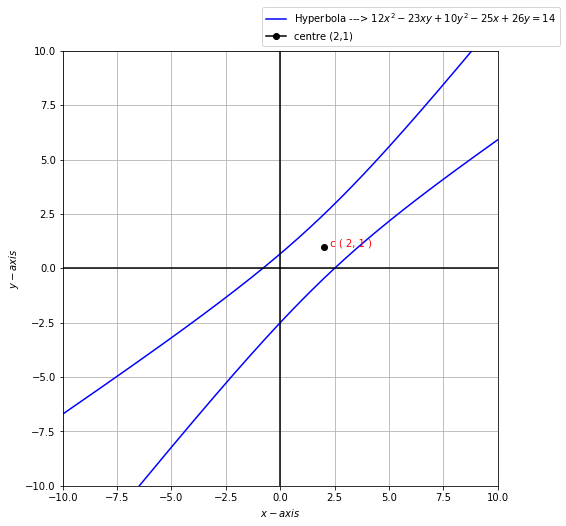
\includegraphics[width=\columnwidth]{./solutions/40/1/Assignment 8.png}
    \caption{Hyperbola when origin is shifted}
    \label{eq:solutions/40/1/Fig :1}
\end{figure}

The figure \ref{eq:solutions/40/1/Fig :1} verifies the given equation \eqref{eq:solutions/40/1/given} as hyperbola with centre $\myvec{2\\1}$



\item What conic does the following equation represent. 
\begin{align}
13x^2-18xy+37y^2+2x+14y-2 = 0
\end{align}
Find the center.
\\
\solution
The general second degree equation can be expressed as follows,
\begin{align}
\vec{x^T}\vec{V}\vec{x}+2\vec{u^T}\vec{x}+f=0\label{eq:solutions/15/40/2/eqmain}
\end{align}
From the given second degree equation we get,
\begin{align}
\vec{V} &= \myvec{13&-9\\-9&37}\\
\vec{u} &= \myvec{1\\7}\\
f &= -2
\end{align}
Expanding the determinant of $\vec{V}$ we observe, 
\begin{align}
\mydet{13&-9\\-9&37} = 400>0 \label{eq:solutions/15/40/2/eqV}
\end{align}
Hence from \eqref{eq:solutions/15/40/2/eqV} we conclude that given equation is an ellipse. The characteristic equation of $\vec{V}$ is given as follows,
\begin{align}
\mydet{\lambda\vec{I}-\vec{V}} = \mydet{\lambda-13&9\\9&\lambda-37} &= 0\\
\implies \lambda^2-50\lambda+400 &= 0\label{eq:solutions/15/40/2/eqchar}
\end{align}
Hence the characteristic equation of $\vec{V}$ is given by \eqref{eq:solutions/15/40/2/eqchar}. The roots of \eqref{eq:solutions/15/40/2/eqchar} i.e the eigenvalues are given by
\begin{align}
\lambda_1=10, \lambda_2=40\label{eq:solutions/15/40/2/eqeigenvals}    
\end{align}
The eigen vector $\vec{p}$ is defined as, 
\begin{align}
\vec{V}\vec{p} &= \lambda\vec{p}\\
\implies\brak{\lambda\vec{I}-\vec{V}}\vec{p}&=0
\end{align}
for $\lambda_1=10$,
\begin{align}
\brak{\lambda_1\vec{I}-\vec{V}}&=\myvec{-3&9\\9&-27}\xleftrightarrow[R_1=\frac{1}{3}R_1]{R_2=R_2+3R_1}\myvec{-1&3\\0&0}\\
\implies\vec{p_1}&=\myvec{3\\1}
\end{align}
Again, for $\lambda_2=40$,
\begin{align}
\brak{\lambda_2\vec{I}-\vec{V}}&=\myvec{27&9\\9&3}\xleftrightarrow[R_1=\frac{1}{27}R_1]{R_2=R_2-R_1}\myvec{1&\frac{1}{3}\\0&0}\\
\implies\vec{p_2}=\myvec{-1\\3}
\end{align}
Again, 
Hence from the equation
\begin{align}
\vec{V}&=\vec{P}\vec{D}\vec{P^{-1}}
%\intertext{Where $\vec{D}$ is a diagonal matrix, we get,}
\vec{P}&=\myvec{\vec{p_1}&\vec{p_2}}=\myvec{3&-1\\1&3}\\
\vec{D}&=\myvec{10&0\\0&40}
\end{align}
Now \eqref{eq:solutions/15/40/2/eqmain} can be written as,
\begin{align}
\vec{y^T}\vec{D}\vec{y}&=\vec{u^T}\vec{V^{-1}}\vec{u}-f\qquad\text{$\mydet{\vec{V}}\not=0$}\label{eq:solutions/15/40/2/eqnewmain}\\
\intertext{And,}
\vec{c}&= -\vec{V^{-1}}\vec{u}\qquad\text{$\mydet{\vec{V}}\not=0$}\label{eq:solutions/15/40/2/eqcenter}\\
\vec{y} &= \vec{P^T}\brak{\vec{x-c}}\label{eq:solutions/15/40/2/eqY}
\end{align}
The centre/vertex of the conic section in \eqref{eq:solutions/15/40/2/eqmain} is given by $\vec{c}$ in \eqref{eq:solutions/15/40/2/eqcenter}. 
We compute $\vec{V^{-1}}$ as follows,
\begin{align}
\myvec{13&-9&1&0\\-9&37&0&1}&\xleftrightarrow[R_2=\frac{13}{400}R_2]{R_2=R_2+\frac{9}{13}R_1}\myvec{13&-9&1&0\\0&1&\frac{9}{400}&\frac{13}{400}}\\
&\xleftrightarrow[R_1=R_1+\frac{9}{13}R_2]{R_1=\frac{1}{13}R_1}\myvec{1&0&\frac{37}{400}&\frac{9}{400}\\0&1&\frac{9}{400}&\frac{13}{400}}
\end{align}
Hence $\vec{V^{-1}}$ is given by,
\begin{align}
\vec{V^{-1}} = \myvec{\frac{37}{400}&\frac{9}{400}\\\frac{9}{400}&\frac{13}{400}}
\end{align}
Now $\vec{u^T}\vec{V^{-1}}\vec{u}$ is given by,
\begin{align}
\vec{u^T}\vec{V^{-1}}\vec{u}&=\frac{1}{400}\myvec{1&7}\myvec{37&9\\9&13}\myvec{1\\7}=2\label{eq:solutions/15/40/2/eqRHS}\\
\intertext{And, $\vec{V^{-1}}\vec{u}$ is given by,}
\vec{V^{-1}}\vec{u} &= \frac{1}{400}\myvec{100\\100}=\frac{1}{4}\myvec{1\\1}\label{eq:solutions/15/40/2/eqcenterRHS}
\end{align}
By putting the value of \eqref{eq:solutions/15/40/2/eqcenterRHS}, the center of the ellipse is given by \eqref{eq:solutions/15/40/2/eqcenter} as follows,
\begin{align}
\vec{c} = -\frac{1}{4}\myvec{1\\1} = \myvec{-\frac{1}{4}\\-\frac{1}{4}}
\end{align}
Also the semi-major axis ($a$) and semi-minor axis ($b$) of the ellipse are given by,
\begin{align}
a = \sqrt{\frac{\vec{u^T}\vec{V^{-1}}\vec{u}-f}{\lambda_1}}=\frac{\sqrt{10}}{5}\\
b = \sqrt{\frac{\vec{u^T}\vec{V^{-1}}\vec{u}-f}{\lambda_2}}=\frac{\sqrt{10}}{10}
\end{align}
Finally from \eqref{eq:solutions/15/40/2/eqnewmain}, the equation of ellipse is given by,
\begin{align}
&\vec{y^T}\myvec{10&0\\0&40}\vec{y}=4\label{eq:solutions/15/40/2/eqFinal}
\end{align}

The following figure \ref{eq:solutions/15/40/2/fig:my_label}
is the graphical representation of the ellipse in \eqref{eq:solutions/15/40/2/eqFinal},
\begin{figure}[t]
\centering
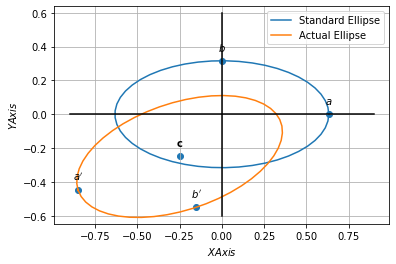
\includegraphics[width = \columnwidth]{./solutions/40/2/Ellipse.png}
\caption{Graphical representation of the ellipse}
\label{eq:solutions/15/40/2/fig:my_label}
\end{figure}


%
\item What conic does the following equation represent?
\begin{align}
y^2-2\sqrt{3}xy+3x^2+6x-4y+5 = 0
\end{align}
Find the center.
\\
\solution
The general second degree equation can be expressed as follows,
\begin{align}
\vec{x^T}\vec{V}\vec{x}+2\vec{u^T}\vec{x}+f=0\label{eq:solutions/40/3/eqmain}
\end{align}
From the given second degree equation we get,
\begin{align}
\vec{V} &= \myvec{3&-\sqrt{3}\\-\sqrt{3}&1}\\ \label{eq:solutions/40/3/given1}
\vec{u} &= \myvec{3\\-2}\\ 
f &= 5 \label{eq:solutions/40/3/given2}
\end{align}
Expanding the determinant of $\vec{V}$ we observe, 
\begin{align}
\mydet{3&-\sqrt{3}\\-\sqrt{3}&1} = 0 \label{eq:solutions/40/3/eq2.1}
\end{align}
Also
\begin{align}
    \mydet{\vec{V}&\vec{u} \\\vec{u}^T & f}=
    \mydet{3&-\sqrt{3}&3\\-\sqrt{3}&1 &-2\\3 &-2&5}
    \neq 0\label{eq:solutions/40/3/eq2.2}\end{align}
Hence from \eqref{eq:solutions/40/3/eq2.1} and \eqref{eq:solutions/40/3/eq2.2} we conclude that given equation is a parabola. The characteristic equation of $\vec{V}$ is given as follows,
\begin{align}
\mydet{\vec{V}-\lambda\vec{I}} = \mydet{3-\lambda &-\sqrt{3}\\-\sqrt{3}& 1-\lambda} &= 0\\
\implies \lambda^2-4\lambda &= 0\label{eq:solutions/40/3/eqchar}
\end{align}
Hence the characteristic equation of $\vec{V}$ is given by \eqref{eq:solutions/40/3/eqchar}. The roots of \eqref{eq:solutions/40/3/eqchar} i.e the eigenvalues are given by
\begin{align}
\lambda_1=0, \lambda_2=4\label{eq:solutions/40/3/eqeigenvals}    
\end{align}
The eigen vector $\vec{p}$ is defined as, 
\begin{align}
\vec{V}\vec{p} &= \lambda\vec{p}\\
\implies\brak{\vec{V}-\lambda\vec{I}}\vec{p}&=0 \label{eq:solutions/40/3/eqev}
\end{align}
for $\lambda_1=0$,
\begin{align}
\brak{\vec{V}-\lambda_1\vec{I}}&=\myvec{3&-\sqrt{3}\\-\sqrt{3}&1}\xleftrightarrow[R_1=\frac{1}{\sqrt{3}}R_1]{R_2=R_1+R_2}\myvec{\sqrt{3}&-1\\0&0}\label{eq:solutions/40/3/eq2.3.0}
\end{align}
Substiuting equation \ref{eq:solutions/40/3/eq2.3.0} in equation \ref{eq:solutions/40/3/eqev} and upon normalizing we get we get
\begin{align}
\implies\vec{p_1}&=\myvec{1/2\\\sqrt{3}/2} \label{eq:solutions/40/3/eq2.3}
\end{align}
Again, for $\lambda_2=4$,
\begin{align}
\brak{\vec{V}-\lambda_2\vec{I}}&=\myvec{-1&-\sqrt{3}\\-\sqrt{3}&-3}\xleftrightarrow[R_1=-\sqrt{3}R_1]{R_2=-\sqrt{3}R_1+R_2}\myvec{1&\sqrt{3}\\0&0} \label{eq:solutions/40/3/eq2.3.1}
\end{align}
Substiuting equation \ref{eq:solutions/40/3/eq2.3.1} in equation  \ref{eq:solutions/40/3/eqev} and upon normalizing we get
\begin{align}
        \vec{p_2}&=\myvec{-\sqrt{3}/2 \\1/2} \label{eq:solutions/40/3/eqp1}
\end{align}
The matrix $\vec{P}$,
\begin{align}
\vec{P}&=\myvec{\vec{p_1}&\vec{p_2}}=\myvec{1/2&-\sqrt{3}/2\\\sqrt{3}/2&1/2} \\
\vec{D}&=\myvec{0&0\\0&4}
\end{align}
\begin{align}
    \eta=2\vec{p_1}^T\vec{u}=3-2\sqrt{3} 
\end{align}
The focal length of the parabola is given by:
\begin{align}
    \abs{\frac{\eta}{\lambda_2}} 
    = \abs{\frac{3-2\sqrt{3}}{4}} = 0.116
\end{align}
When $\mydet{\vec{V}}=0$, \eqref{eq:solutions/40/3/eqmain} can be written as
\begin{align}
    \vec{y^T}\vec{D}\vec{y}&=-\eta\myvec{1&0}\vec{y}\label{eq:solutions/40/3/eq2.4}
    \intertext{And the vertex $\vec{c}$ is given by }
    \myvec{\vec{u^T}+\frac{\eta}{2}\vec{p_1^T} \\ \vec{V}}\vec{c}=
    \myvec{-f \\ \frac{\eta}{2}\vec{p_1}-\vec{u}}\label{eq:solutions/40/3/eqa} 
\end{align}
Substituting the found values
\begin{align}
\vec{u}^T + \frac{\eta}{2}\vec{p_1}^T = \myvec{3&-2}+\frac{3-2\sqrt{3}}{2}\myvec{\frac{1}{2}&\frac{\sqrt{3}}{2}}\\
\implies\vec{u}^T + \frac{\eta}{2}\vec{p_1}^T =\myvec{\frac{15-2\sqrt{3}}{4}&\frac{-14+3\sqrt{3}}{4}}\label{eq:solutions/40/3/eq2.23} \\
\frac{\eta}{2} \vec{p_1} -\vec{u}= \myvec{\frac{-9-2\sqrt{3}}{4}\\ \frac{2+3\sqrt{3}}{4}}\label{eq:solutions/40/3/eq2.24}
\end{align}
using equations \eqref{eq:solutions/40/3/given1},\eqref{eq:solutions/40/3/given2},\eqref{eq:solutions/40/3/eq2.3},\eqref{eq:solutions/40/3/eq2.23},\eqref{eq:solutions/40/3/eq2.24} and \eqref{eq:solutions/40/3/eq2.3} in \eqref{eq:solutions/40/3/eqa}
\begin{align}
    \myvec{\frac{15-2\sqrt{3}}{4}&\frac{-14+3\sqrt{3}}{4}\\3 & -\sqrt{3}\\ -\sqrt{3}& 1}\vec{c} =\myvec{ -5\\\frac{-9-2\sqrt{3}}{4}\\ \frac{2+3\sqrt{3}}{4}}\label{eq:solutions/40/3/eqcen}
\end{align}
By performing row reductions on augmented matrix
\begin{multline}
\myvec{\frac{15-2\sqrt{3}}{4}&\frac{-14+3\sqrt{3}}{4}&-5\\3 & -\sqrt{3}&\frac{(-9-2\sqrt{3})}{4}\\ -\sqrt{3}& 1&\frac{2+3\sqrt{3}}{4}}{R_2\xleftrightarrow[]{}{R_1}}\\
\myvec{3 & -\sqrt{3}&\frac{(-9-2\sqrt{3})}{4}\\\frac{15-2\sqrt{3}}{4}&\frac{-14+3\sqrt{3}}{4}&-5\\-\sqrt{3}& 1&\frac{2+3\sqrt{3}}{4} }
\end{multline}
\begin{multline}
\myvec{3 & -\sqrt{3}&\frac{(-9-2\sqrt{3})}{4}\\\frac{15-2\sqrt{3}}{4}&\frac{-14+3\sqrt{3}}{4}&-5\\-\sqrt{3}& 1&\frac{2+3\sqrt{3}}{4}}
\xleftrightarrow[]{R_2\leftarrow R_2-\frac{15-2\sqrt{3}}{12}R_1}\\
\myvec{3 & -\sqrt{3}&\frac{(-9-2\sqrt{3})}{4}\\0 & 2(\sqrt{3}-2) & \frac{(4\sqrt{3}-39)}{16}\\\sqrt{3}& 1&\frac{2+3\sqrt{3}}{4}}
\end{multline}
Therefore, 
\begin{multline}
 \myvec{3 & -\sqrt{3}&\frac{(-9-2\sqrt{3})}{4}\\0&2(\sqrt{3}-2)&\frac{(4\sqrt{3}-39)}{16}\\-\sqrt{3}& 1&\frac{(2+3\sqrt{3})}{4}}\xleftrightarrow[]{R_3\leftarrow R_3+\frac{1}{\sqrt{3}}R_1}\\
\myvec{3 & -\frac{433}{250}&-\frac{311}{100}\\0 & -\frac{107}{200} & -2\\0& 0&0}
\end{multline}
\begin{figure}[!h]
    \centering
    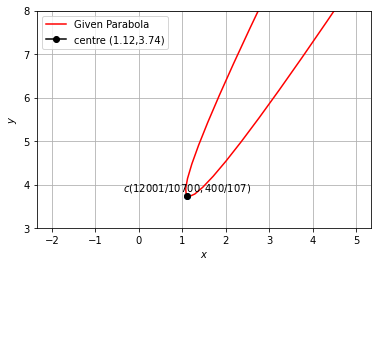
\includegraphics[width=\columnwidth]{./solutions/40/3/parabola.png}
    \caption{Parabola with the center c}
    \label{eq:solutions/40/3/Fig:1}
\end{figure}
\begin{multline}
\myvec{3 & -\frac{433}{250}&-\frac{311}{100}\\0 & -\frac{107}{200} & -2\\0& 0&0}\xleftrightarrow[]{R_1\leftarrow \frac{R_1}{{3}}}\\\myvec{1& -\frac{433}{750}&-\frac{311}{300}\\0 & -\frac{107}{200} & -2\\0& 0&0}
\end{multline}
\begin{multline}
\myvec{1 & -\frac{433}{750}&-\frac{311}{300}\\0 & -\frac{107}{200} & -2\\0& 0&0}\xleftrightarrow[]{R_2\leftarrow \frac{-200}{{107}}R_2}\\
\myvec{1 & -\frac{433}{750}&-\frac{311}{300}\\0 & 1 & \frac{400}{107}\\0& 0&0}
\end{multline}

\begin{multline}
\myvec{1 & -\frac{433}{750}&-\frac{311}{300}\\0 & 1 & \frac{400}{107}\\0& 0&0}\xleftrightarrow[]{R_1\leftarrow R_1+\frac{433}{{750}}R_2}\\
\myvec{1 & 0&\frac{12001}{10700}\\0 & 1 & \frac{400}{107}\\0& 0&0}\label{eq:solutions/40/3/eq7}
\end{multline}
On solving for values of $\vec{c}$ from \eqref{eq:solutions/40/3/eq7} 
 The vertex of parabola is $\vec{c}$=$\myvec{\frac{12001}{10700}\\\frac{400}{107}}$.
 

\item What conics do the following equation represent? When possible, find the centres and also their equations referred to the centre.
\begin{align}
2x^2-72xy+23y^2-4x-2y-48=0\label{eq:solutions/40/4/ques}
\end{align}
\solution
%
The second degree equation in general can be represented as
\begin{align}
    ax^2+2bxy+cy^2+2dx+2ey+f=0\label{eq:solutions/40/4/general}
\end{align}
The equation \eqref{eq:solutions/40/4/general} in matrix form can be represented as 
\begin{align}
%&\vec{x}^T\myvec{12 & \frac{-23}{2}\\\frac{-23}{2} & %10}\vec{x}+2\myvec{\frac{-25}{2} & 13}\vec{x}-14=0\label{eq:solutions/40/4/given}
\vec{x}^T\vec{V}\vec{x}+2\vec{u}^T\vec{x}+f=0\label{eq:solutions/40/4/given}
\end{align}
where 
\begin{align}
\vec{V}=\myvec{a&b\\b&c}=\myvec{2 & -36\\-36 & 23}\\
\vec{u}=\myvec{d\\e}=\myvec{-2 \\ -1}\\
f=-48
\end{align}
\begin{align}
    \det(\vec{V})=\begin{array}{|cc|} 2 & -36\\-36 & 23 \end{array}\\
\implies\det(\vec{V})=-1250\\
\implies\det(\vec{V})<0
\end{align}
Since $\det(\vec{V})<0$ the given equation \eqref{eq:solutions/40/4/ques} represents a hyperbola. The characteristic equation of $\vec{V}$ is acquired by evaluating the determinant 
\begin{align}
       \begin{array}{|c|}
V-\lambda\vec{I}
\end{array}=0\\
   \begin{array}{|cc|}
2-\lambda & -36 \\ -36 & 23-\lambda
\end{array}=0\\
\implies \lambda^2-25\lambda-1250=0\label{eq:solutions/40/4/eqroots}
\end{align}
On solving the equation \eqref{eq:solutions/40/4/eqroots}, the eigen values are given by 
\begin{align}
    \lambda_1=50\label{eq:solutions/40/4/eqeig1}\\
    \lambda_2=-25\label{eq:solutions/40/4/eqeig2}
\end{align}
We can observe that for a hyperbola, $\lambda_1>0$ and  $\lambda_2<0$.
Consider the eigenvector $\vec{p}=\myvec{v_1\\v_2}$ is defined as 
\begin{align}
    \vec{V}\vec{p}&=\lambda\vec{p}\\
    \implies (\vec{V}-\lambda\vec{I})\vec{p}&=0\label{eq:solutions/40/4/cheq}
\end{align}
For $\lambda_1=50$ ,
\begin{align}
    (\vec{V}-\lambda_1\vec{I})=\myvec{-48&-36\\-36&-27}
\end{align}
By row reduction , 
\begin{align}
    \myvec{-48&-36\\-36&-27}\\
    \xleftrightarrow[R_1\leftarrow\frac{R_1}{-12}]{R_2\leftarrow\frac{R_2}{-9}}\myvec{4&3\\4&3}\\
    \xleftrightarrow[]{R_2\leftarrow R_2-R_1}
    \myvec{4&3\\0&0}\label{eq:solutions/40/4/ref1}
\end{align}
Subsituting equation \eqref{eq:solutions/40/4/ref1} in equation \eqref{eq:solutions/40/4/cheq} we get
\begin{align}
        \myvec{4&3\\0&0}\myvec{v_1\\v_2}=\myvec{0\\0}\label{eq:solutions/40/4/eig1}
\end{align}
Eigen vector $\vec{p_1}$ is given by
\begin{align}
    \vec{p_1}=\myvec{\frac{-3}{4}\\1}\label{eq:solutions/40/4/ev1}
\end{align}
For $\lambda_2=-25$ ,
\begin{align}
    (\vec{V}-\lambda_2\vec{I})=\myvec{27&-36\\-36&48}
\end{align}
By row reduction , 
\begin{align}
    \myvec{27&-36\\-36&48}\\
    \xleftrightarrow[R_1\leftarrow\frac{R_1}{9}]
    {R_2\leftarrow\frac{R_2}{-12}}
    \myvec{3&-4\\3&-4}\\
    \xleftrightarrow[]{R_2\leftarrow R_2-R_1}
    \myvec{3&-4\\0&0}\label{eq:solutions/40/4/ref2}
\end{align} 
Subsituting equation \eqref{eq:solutions/40/4/ref2} in equation \eqref{eq:solutions/40/4/cheq} we get 
\begin{align}
    \myvec{3&-4\\0&0}\myvec{v_1\\v_2}=\myvec{0\\0}\label{eq:solutions/40/4/eig2}
\end{align}
Eigen vector $\vec{p_2}$ is given by
\begin{align}
        \vec{p_2}=\myvec{\frac{4}{3}\\1}\label{eq:solutions/40/4/ev2}
\end{align}
By eigen decompostion, $\vec{V}$ can be represented by
\begin{align}
    \vec{V}=\vec{P}\vec{D}\vec{P}^T\label{eq:solutions/40/4/evd}
\end{align}
where 
\begin{align}
        \vec{P}=\myvec{\vec{p_1} & \vec{p_2}}\label{eq:solutions/40/4/eqp}\\
    \vec{D}=\myvec{\lambda_1 & 0 \\0 & \lambda_2}\label{eq:solutions/40/4/eqD}
\end{align}
Substituting equations \eqref{eq:solutions/40/4/ev1}, \eqref{eq:solutions/40/4/ev2} in equation \eqref{eq:solutions/40/4/eqp} we get 
\begin{align}
    \vec{P}=\myvec{\frac{-3}{4}&\frac{4}{3}\\1&1}\label{eq:solutions/40/4/eqP}
\end{align}
Substituting equations \eqref{eq:solutions/40/4/eqeig1}, \eqref{eq:solutions/40/4/eqeig2} in \eqref{eq:solutions/40/4/eqD} we get
\begin{align}
       \vec{D}=\myvec{50 & 0\\0 & -25}\label{eq:solutions/40/4/eqDD}
\end{align}
Centre of the hyperbola is given by 
\begin{align}
    \vec{c}=-\vec{V}^{-1}\vec{u}
\end{align}
\begin{align}
    \implies\vec{c}=-\myvec{\frac{-23}{1250}&\frac{-18}{625}\\\frac{-18}{625}&\frac{-1}{625}}\myvec{-2\\-1}\\
    \implies\vec{c}=\myvec{\frac{-41}{625}\\\frac{-37}{625}}
\end{align}
Since,
\begin{align}
    \vec{u}^T\vec{V}^{-1}\vec{u}-f = \frac{-30119}{625}<0\label{eq:solutions/40/4/cond}
\end{align} 
We swap the semi-major and semi-minor axes and the respective are given by
\begin{align}
axes=
\begin{cases}
\sqrt{\frac{\vec{u}^T\vec{V}^{-1}\vec{u}-f}{\lambda_2}}\\ \sqrt{\frac{f-\vec{u}^T\vec{V}^{-1}\vec{u}}{\lambda_1}}
\end{cases}
\end{align}
Calculating the axes, we get
\begin{align}
\sqrt{\frac{\vec{u}^T\vec{V}^{-1}\vec{u}-f}{\lambda_2}}=1.388\\
\sqrt{\frac{f-\vec{u}^T\vec{V}^{-1}\vec{u}}{\lambda_1}}=0.981
\end{align}
The figure \ref{eq:solutions/40/4/Fig :1} verifies the given equation \eqref{eq:solutions/40/4/given} as hyperbola with centre $\myvec{\frac{-41}{625}\\\frac{-37}{625}}$
\begin{figure}[h]
    \centering
    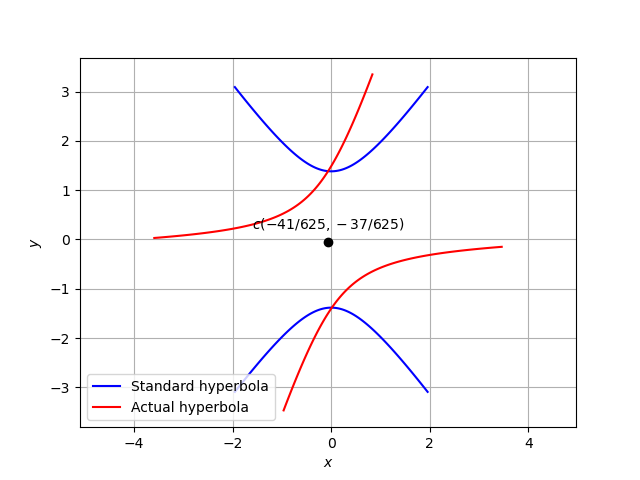
\includegraphics[width=\columnwidth]{./solutions/40/4/Hyperbola.png}
    \caption{Hyperbola when origin is shifted}
    \label{eq:solutions/40/4/Fig :1}
\end{figure}
\item  Now \eqref{eq:solutions/40/4/given} can be written as,
\begin{align}
    \vec{y}^T\vec{D}\vec{y}=\vec{u}^T\vec{V}^{-1}\vec{u}-f\label{eq:solutions/40/4/fi}
\end{align}
where ,
\begin{align}
    \vec{y}&=\vec{P}^T(\vec{x}-\vec{c})
\end{align}
To get $\vec{y}$,
\begin{align}
    \vec{y}=\vec{P}^T\vec{x}-\vec{P}^T\vec{c}\\
    \vec{y}=\myvec{\frac{-3}{4}&1\\\frac{4}{3}&1}\vec{x}-
    \myvec{\frac{-3}{4}&1\\\frac{4}{3}&1}\myvec{\frac{-41}{625}\\\frac{-37}{625}}\\
    \vec{y}=\myvec{\frac{-3}{4}&1\\\frac{4}{3}&1}\vec{x}-
    \myvec{\frac{-1}{100}\\\frac{-11}{75}}
\end{align}
Subsituting the eqauations \eqref{eq:solutions/40/4/cond}, \eqref{eq:solutions/40/4/eqDD} in equation \eqref{eq:solutions/40/4/fi}
\begin{align}
    \vec{y}^T\myvec{50&0\\0&-25}\vec{y}=\frac{-30119}{625}
\end{align}

\item What conic does the given equations represent?
\begin{align}
6x^2-5xy-6y^2+14x+5y+4=0
\end{align}
\\
\solution
The above equation can be expressed in the form 
\begin{align}
\vec{x}^T\vec{V}\vec{x}+2\vec{u}^T\vec{x}+f&=0 \label{eq:solutions/40/5/eq1}
\intertext{Comparing equation we get}
    \vec{V}=\vec{V}^T&=\myvec{6 & \frac{-5}{2}\\\frac{-5}{2} &-6}\label{eq:solutions/40/5/eqv}\\
    \vec{u}&=\myvec{7 \\ \frac{5}{2}}\label{eq:solutions/40/5/equ}\\
    f&=4\label{eq:solutions/40/5/eqfv}
\end{align}    
The above equation \eqref{eq:solutions/40/5/eq1} represents a pair of straight lines if
\begin{align}
    \begin{array}{|cc|}
\vec{V} & \vec{u}\\\vec{u}^T & f
\end{array}&=0\label{eq:solutions/40/5/eqcheck}
\end{align}
Verify the given equation as if it is pair of straight lines
\begin{align}
\Delta&=\begin{array}{|ccc|}
6 &\frac{-5}{2}& 7\\\frac{-5}{2} & -6 & \frac{5}{2}\\ 7 & \frac{5}{2} & 4
\end{array}\\
\implies \ 6\mydet{-6 & \frac{5}{2} \\ \frac{5}{2} & 4} 
		& -\frac{-5}{2}\mydet{-\frac{5}{2} & \frac{5}{2} \\ 7 & 4}
		+7\mydet{-\frac{5}{2} & -6 \\ 7 & \frac{5}{2}} = 0 \label{eq:solutions/40/5/eq10}\\
\implies \Delta&=0
\end{align}
Since equation \eqref{eq:solutions/40/5/eqcheck} is satisfied, we could say that the given equation represents two straight lines
\begin{align}
    \Delta_{V} &= \begin{array}{|cc|}
6 &\frac{-5}{2}\\\frac{-5}{2} & -6
\end{array}<0
\end{align}
Let the equations of lines be,
\begin{align}
	\brak{\vec{n_1}^T \vec{x} - c_1}\brak{\vec{n_1}^T \vec{x} - c_1} =
        \vec{x}^{T}\vec{Vx} + 2\vec{u}^{T}\vec{x} + f=0\label{eq:solutions/40/5/eq:eql03}
\end{align}
\begin{align}
\brak{\vec{n_1}^T\vec{x}-c_1}\brak{\vec{n_2}^T\vec{x}-c_2}
&=\vec{x}^T\myvec{6 & \frac{-5}{2} \\\frac{-5}{2} & -6}\vec{x}\notag\\
+2\myvec{7 & \frac{5}{2}}\vec{x}+4\label{eq:solutions/40/5/equate}\\
    \vec{n_1}*\vec{n_2} = \myvec{a\\2b\\c} &= \myvec{6\\-5\\-6}\label{eq:solutions/40/5/conv}\\
    c_2\vec{n_1}+c_1\vec{n_2}&=-2\myvec{7\\\frac{5}{2}}\label{eq:solutions/40/5/eqc1c2}\\
    c_1c_2&=4
\end{align}
The slopes of the lines are given by the roots of the polynomial 
\begin{align}
    &cm^2+2bm+a=0\label{eq:solutions/40/5/e}\\
    \implies m_i&=\frac{-b\pm{\sqrt{-\Delta_{V}}}}{c}\\
    \vec{n_i}&=k\myvec{-m_i\\1}
\end{align}
Substituting the given data in above equations \eqref{eq:solutions/40/5/e} we get,
\begin{align}
    &-6m^2-5m+6=0\\
    &\implies m_i=\frac{\frac{-5}{2}\pm{\sqrt{-(\frac{-169}{4})}}}{-6}\label{eq:solutions/40/5/m}
\intertext{Solving equation \eqref{eq:solutions/40/5/m} we get,}
    m_1&=-\frac{3}{2},  m_2=\frac{2}{3}\\
   % \vec{m_1}=\myvec{-2\\3}, \vec{m_2}=\myvec{3\\ 2}\\
   &= \vec{n_1}=\myvec{-3\\ -2}, \vec{n_2}=\myvec{-2\\3} \label{eq:solutions/40/5/eq:normal1}
\intertext{We know that,}
\vec{n_1}\ast \vec{n_2} = \myvec{a\\2b\\c} \label{eq:solutions/40/5/eq:conv1}
\end{align}
Verification using Toeplitz matrix, From equation \eqref{eq:solutions/40/5/eq:normal1}
\begin{align}
    \vec{n_1}=\myvec{-3&0\\-2&-3\\0&-2}
    \vec{n_2}=\myvec{-2\\3}\label{eq:solutions/40/5/eq:conv2}\\
\implies \myvec{-3&0\\-2&-3\\0&-2}\myvec{-2\\ 3} = \myvec{6\\-5\\-6} = \myvec{a\\2b\\c}\label{eq:solutions/40/5/eq:conv3}
\end{align}
$\implies$ Equation \eqref{eq:solutions/40/5/eq:normal1} satisfies \eqref{eq:solutions/40/5/eq:conv1}\\
$c_1$ and $c_2$ can be obtained as,
\begin{align}
\myvec{\vec{n_1} & \vec{n_2}}\myvec{c_2\\c_1}&=-2\vec{u} \label{eq:solutions/40/5/eq:aug1}
\end{align}
Substituting \eqref{eq:solutions/40/5/eq:normal1} in \eqref{eq:solutions/40/5/eq:aug1}, the augmented matrix is,
\begin{align}
\myvec{-3 & -2 & 14 \\ -2 & 3 & 5}
\xleftrightarrow[R_2\leftarrow R_2+2R_1]{R_1\leftarrow -R_1/3}
\myvec{1 &\frac{2}{3} &-\frac{14}{3} \\ 0& \frac{13}{3} & -\frac{13}{3}} \label{eq:solutions/40/5/eq:aug5}\\
\xleftrightarrow[R_1\leftarrow R_1-\frac{2}{3}R_2]{R_2\leftarrow \frac{3}{13}R_2}
\myvec{1 &0 &-4 \\ 0& 1 & -1} \label{eq:solutions/40/5/eq:aug2}\\
\implies c_1 = -4, c_2=-1 \label{eq:solutions/40/5/eq:const1}
\end{align}
Equations \eqref{eq:solutions/40/5/eq:eql03}, can be modified as,from \eqref{eq:solutions/40/5/eq:normal1} and \eqref{eq:solutions/40/5/eq:const1} in we get,
\begin{align}
    \myvec{-3 & -2}\vec{x}&=-4\\
    \myvec{-2 & 3}\vec{x}&=-1
\end{align}
\begin{multline}
\implies \brak{-3x-2y+4}\brak{-2x+3y+1}= 0\\
\implies \boxed{\brak{3x+2y-4}\brak{2x-3y-1} = 0} \label{eq:solutions/40/5/eq:line1}
\end{multline}
The angle between the lines can be expressed as, 
\begin{align}
	\vec{n_1}=\myvec{-3\\-2} , \quad \vec{n_2}=\myvec{-2\\3}\\
	\cos\theta=\frac{\vec{n_1}^T\vec{n_2}}{\norm{\vec{n_1}}\norm{\vec{n_2}}} \\
	\implies \quad \theta=\cos^{-1}({\frac{0}{\sqrt{169}}}) = 90\degree.
\end{align}
\begin{figure}[h]
    \centering
    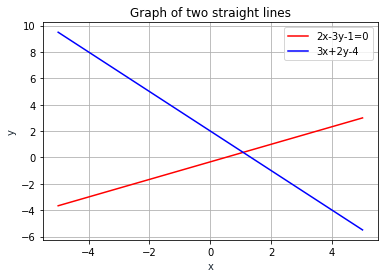
\includegraphics[width=\columnwidth]{./solutions/40/5/A6.png}
    \caption{Pair of straight lines}
    \label{eq:solutions/40/5/Fig :1}
\end{figure}

\item What conic does the following equation represent? Find its equation and centre.
\begin{align*}
	3x^2 - 8xy - 3y^2 + 10x - 13y + 8 =0 
\end{align*}
\solution
The general equation of second degree can be expressed as
\begin{align}
	\vec{x}^{T}\vec{Vx} + 2\vec{u}^{T}\vec{x} + f=0   \label{eq:solutions/40/6/stdsecdeg}
\end{align}
where
\begin{align}
        \vec{V}=\vec{V}^T=\myvec{a & b \\ b & c}   \label{eq:solutions/40/6/V}  \\
        \vec{u}^T=\myvec{d &  e}            \label{eq:solutions/40/6/u}
\end{align}
From (\ref{eq:solutions/40/6/V}) and (\ref{eq:solutions/40/6/u})
\begin{align}
	\vec{V}=\vec{V}^T &= \myvec{3 & -4 \\ -4 & -3} \\
	\vec{u} &= \myvec{5 \\ -\frac{13}{2}}
\end{align}
\begin{align}
	\mydet{\vec{V}}=\mydet{3 & -4 \\ -4 & 3} =-25 \\
	\implies \mydet{\vec{V}} < 0       \label{eq:solutions/40/6/detless0}
\end{align}
Since $ \vec{V} = \vec{V}^T $, there exists an orthogonal matrix $\vec{P}$ such that
\begin{align}
	\vec{P}\vec{V}\vec{P}^T = \vec{D} = diag\myvec{\lambda_1 & \lambda_2}
\end{align}
or equivalently 
\begin{align}
	\vec{V} = \vec{P}\vec{D}\vec{P}^T
\end{align}
Eigen vectors of real symmetric matrix $\vec{V}$ are orthogonal. The characteristic equation of $\vec{V}$ is obtained by evaluating the determinant
\begin{align}
	\mydet{\lambda\vec{I}-\vec{V}} = \mydet{\lambda-3 & 4 \\ 4 & \lambda + 3} = 0 \\
	\implies \quad \lambda^2-25=0 \\
	\implies \quad \lambda_1=-5,\lambda_2=5   \label{eq:solutions/40/6/lambdavals}
\end{align}
From (\ref{eq:solutions/40/6/detless0}) and (\ref{eq:solutions/40/6/lambdavals}) the equation represents a hyperbola.
The eigen vector $\vec{p}$ is defined as
\begin{align}
	\vec{V}\vec{p}=\lambda\vec{p} \\
	\implies (\lambda\vec{I} - \vec{V})\vec{p}=0
\end{align}
For $\lambda_1 = -5$ :
\begin{align}
	(\lambda_1\vec{I}-\vec{V})=\myvec{-8 & 4 \\ 4 & -2} 
	\xleftrightarrow[R_2 \leftarrow \frac{R_2}{2}]{R_1 \leftarrow -\frac{R_1}{4}}
	\myvec{2 & -1 \\ 2 & -1} \\
	\xleftrightarrow[]{R_2 \leftarrow R_2 - R_1}
	\myvec{2 & -1 \\ 0 & 0} \\
	\implies \vec{p_1}=\frac{1}{\sqrt{5}}\myvec{2 \\ 1}
\end{align}
Similarly, the eigenvector corresponding to $\lambda_2$ can be obtained as
\begin{align}
	\vec{p_2}=\frac{1}{\sqrt{5}}\myvec{-1\\2}
\end{align}
The orthogonal eigen-vector matrix
\begin{align}
	\vec{P}=\myvec{\vec{p_1} & \vec{p_2}}
	=\frac{1}{\sqrt{5}}\myvec{2 & -1 \\ 1 & 2} \\
	\vec{D}=\myvec{-5 & 0 \\ 0 & 5}
\end{align}
Let $\vec{x}=\vec{P}\vec{y} + \vec{c} $ with $\vec{c}=-\vec{V}^{-1}\vec{u}$. Substituting in (\ref{eq:solutions/40/6/stdsecdeg})
\begin{align}
	\vec{y}^T\vec{D}\vec{y}=\vec{u}^T\vec{V}^{-1}\vec{u}-f 
\end{align}
with centre
\begin{align}
	\vec{c}=-\vec{V^{-1}u}=\myvec{-\frac{41}{25} \\ \frac{1}{50}} 
\end{align}
and minor and major axes parameters as
\begin{align}
	\sqrt{\frac{\lambda_1}{f-\vec{u^{T}V^{-1}u}}} = \sqrt{\frac{500}{33}}, \
	\sqrt{\frac{\lambda_2}{\vec{u^{T}V^{-1}u}-f}} = \sqrt{\frac{500}{33}}
\end{align}
The equation of hyperbola is
\begin{align}
	\frac{y_2^2}{\frac{33}{500}}-\frac{y_1^2}{\frac{33}{500}}=1
\end{align}
\begin{figure}[!h]
	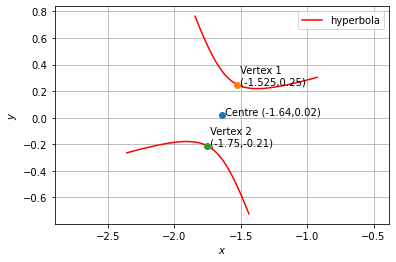
\includegraphics[width=\columnwidth]{./solutions/40/6/hyper.png}
	\caption{} \label{eq:solutions/40/6/linefig1}
\end{figure}

%
\item Find the asymptotes of the hyperbola given below and also the equations to their conjugate hyperbolas.\\
$8x^2+10xy-3y^2-2x+4y-2=0$
%
\solution
The above equation can be expressed in the form 
\begin{align}
\vec{x}^T\vec{V}\vec{x}+2\vec{u}^T\vec{x}+f&=0
%\label{eq:solutions/40/7/2.2} 
\label{eq:solutions/40/7/eq1}
\intertext{Comparing equation we get}
    \vec{V}=\vec{V}^T&=\myvec{8 & 5 \\ 5 &-3}\label{eq:solutions/40/7/eqv}\\
    \vec{u}&=\myvec{-1 \\2 }\label{eq:solutions/40/7/equ}\\
    f&=-2\label{eq:solutions/40/7/eqfv}
\end{align}   
Expanding the Determinant of $\vec{V}$.
\begin{align}
    \Delta_{V} &= \begin{array}{|cc|}
8 &5\\5 & -3
\end{array}<0\label{eq:solutions/40/7/eq:hyp}
\end{align}
Hence from \eqref{eq:solutions/40/7/eq:hyp} given
equation represents the hyperbola
The characteristic equation of $\vec{V}$ is obtained by evaluating the determinant 
\begin{align}
       \begin{array}{|c|}
V-\lambda\vec{I}
\end{array}&=0\\
   \begin{array}{|cc|}
8-\lambda & 5 \\ 5 & -3-\lambda
\end{array}&=0\\
    \brak{8-\lambda}\brak{-3-\lambda}-25=0\\
    \lambda_{1}= \frac{5+\sqrt{221}}{2}\label{eq:solutions/40/7/eq:matrix_l1}\\
    \lambda_{2}= \frac{5-\sqrt{221}}{2}\label{eq:solutions/40/7/eq:matrix_l2}
\end{align}
The eigenvector $\vec{p}$ is defined as 
\begin{align}
    \vec{V}\vec{p}&=\lambda\vec{p}\\
    \implies (\vec{V}-\lambda\vec{I})\vec{p}&=0\label{eq:solutions/40/7/eq:7/eqev}
\end{align}
For $\lambda_1=\frac{5+\sqrt{221}}{2}$ ,
\begin{align}
    (\vec{V}-\lambda_1\vec{I})=\myvec{\frac{11-\sqrt{221}}{2} & 5 \\5 & \frac{-11-\sqrt{221}}{2}}
\end{align}
By row reduction , 
\begin{align}
    &\myvec{\frac{11-\sqrt{221}}{2} & 5 \\5 & \frac{-11-\sqrt{221}}{2}}\\
    %&\xleftrightarrow{\frac{R_1}{\frac{\sqrt{533}+2}{2}}}\\
    &\xleftrightarrow{R_1\leftarrow R_2}
    \myvec{\frac{-11-\sqrt{221}}{2} & 5 \\ \frac{11-\sqrt{221}}{2} & 5}\\
 &\xleftrightarrow{R_2\leftarrow R_2-\frac{11-\sqrt{221}}{10}R_{1}}
    \myvec{5 & \frac{-11-\sqrt{221}}{2} \\ 0& 0}\\
     &\xleftrightarrow{R_1\leftarrow R_1/5}
    \myvec{1 & \frac{-11-\sqrt{221}}{10} \\ 0& 0}
    \label{eq:solutions/40/7/eq:7/eqs1}
\end{align}
Subsituting equation \ref{eq:solutions/40/7/eq:7/eqs1} in equation \ref{eq:solutions/40/7/eq:7/eqev} we get
\begin{align}
        & \myvec{1 & \frac{-11-\sqrt{221}}{10} \\ 0& 0}\myvec{v_1 \\ v_2}=\myvec{0 \\ 0}\label{eq:solutions/40/7/eq:7/eqei1}
\end{align}
Where, $\vec{p}=\myvec{v_1\\v_2}$
Let $v_2=t$
\begin{align}
    v_1&=\frac{t(11+\sqrt{221})}{10}
\end{align}
Eigen vector $\vec{p_1}$ is given by
\begin{align}
    \vec{p_1}&=\myvec{\frac{t(11+\sqrt{221})}{10} \\ t}
\end{align}
Let $t=1$, we get
\begin{align}
        \vec{p_1}&=\myvec{\frac{11+\sqrt{221}}{10} \\1 }\label{eq:solutions/40/7/eq:es71/eqp1}
\end{align}
For $\lambda_2=\frac{5-\sqrt{221}}{2}$ ,
\begin{align}
    (\vec{V}-\lambda_2\vec{I})=\myvec{\frac{11+\sqrt{221}}{2} & 5 \\5 & \frac{-11+\sqrt{221}}{2}}
\end{align}
By row reduction , 
\begin{align}
     \myvec{\frac{11+\sqrt{221}}{2} & 5 \\5 & \frac{-11+\sqrt{221}}{2}}
    \xleftrightarrow{R_1\leftarrow R_2+ \frac{11-\sqrt{221}}{10}R_1}
     \myvec{\frac{11+\sqrt{221}}{2} &5\\ 0& 0}\\  
 \xleftrightarrow{R_1\leftarrow
 \frac{R_1}{\frac{11+\sqrt{221}}{10}}}
    \myvec{1 & \frac{10}{11+\sqrt{221}} \\ 0& 0}
    \label{eq:solutions/40/7/eq:es71/eqs2}
\end{align} 
Substiuting equation \ref{eq:solutions/40/7/eq:es71/eqs2} in equation \ref{eq:solutions/40/7/eq:7/eqev} we get 
\begin{align}
    &\myvec{1 & \frac{10}{11+\sqrt{221}} \\0 & 0}\myvec{v_1 \\ v_2}=\myvec{0 \\ 0}
%\label{eq:solutions/40/7/eq:es71/eqei1}
\end{align}
Where, $\vec{p}=\myvec{v_1\\v_2}$
Let $v_2=t$
\begin{align}
    v_1&=\frac{-t\brak{10}}{11+\sqrt{221}}
\end{align}
Eigen vector $\vec{p_2}$ is given by
\begin{align}
        \vec{p_2}&=\myvec{\frac{-t\brak{10}}{11+\sqrt{221}} \\ t}
\end{align}
Let $t=1$, we get 
\begin{align}
    \vec{p_2}&=\myvec{\frac{\brak{-10}}{11+\sqrt{221}} \\1 }\label{eq:solutions/40/7/eq:es71/eqp2}
\end{align}
By eigen decompostion $\vec{V}$ can be represented by
\begin{align}
    \vec{V}&=\vec{P}\vec{D}\vec{P}^T\label{eq:solutions/40/7/eq:es71/eqsubs}
\end{align}
where 
\begin{align}
        \vec{P}&=\myvec{\vec{p_1} & \vec{p_2}}\label{eq:solutions/40/7/eq:es71/eqp}\\
    \vec{D}&=\myvec{\lambda_1 & 0 \\0 & \lambda_2}\label{eq:solutions/40/7/eq:es71/eqD}
\end{align}
Substituting equations \ref{eq:solutions/40/7/eq:es71/eqp1}, \ref{eq:solutions/40/7/eq:es71/eqp2} in equation \ref{eq:solutions/40/7/eq:es71/eqp} we get 
\begin{align}
    \vec{P}&=\myvec{\frac{11+\sqrt{221}}{10} & \frac{-10}{11+\sqrt{221}} \\1 & 1}\label{eq:solutions/40/7/eq:es71/eqP}
\end{align}
Substituting equations \ref{eq:solutions/40/7/eq:matrix_l1}, \ref{eq:solutions/40/7/eq:matrix_l2} in \ref{eq:solutions/40/7/eq:es71/eqD} we get
\begin{align}
       \vec{D}&=\myvec{\frac{5+\sqrt{221}}{2} & 0\\0 & \frac{5-\sqrt{221}}{2}}\label{eq:solutions/40/7/eq:es71/eqDD}
\end{align}
Centre of the hyperbola is given by 
\begin{align}
    \vec{c}&=-\vec{V}^{-1}\vec{u}\\
    \implies\vec{c}&=-\myvec{\frac{3}{49}&\frac{5}{49}\\\frac{5}{49}&\frac{-8}{49}}\myvec{-1 \\ 2}\\
    \implies\vec{c}&=\myvec{\frac{-3}{49}&\frac{-5}{49}\\\frac{-5}{49}&\frac{8}{49}}\myvec{-1 \\ 2}\\
    \implies\vec{c}&=\myvec{\frac{-1}{7}\\\frac{3}{7}}
\end{align}
Since,
\begin{align}
    \vec{u}^T\vec{V}^{-1}\vec{u}-f = 1 > 0\label{eq:solutions/40/7/eq:es71/cond}
\end{align} 
there isn't a need to swap axes
In hyperbola,
\begin{align}
axes=
\begin{cases}
\sqrt{\frac{\vec{u}^T\vec{V}^{-1}\vec{u}-f}{\lambda_1}}\\ \sqrt{\frac{f-\vec{u}^T\vec{V}^{-1}\vec{u}}{\lambda_2}}
\end{cases}
\end{align}
From above equations we can say that,
\begin{align}
\sqrt{\frac{\vec{u}^T\vec{V}^{-1}\vec{u}-f}{\lambda_1}}=\sqrt{ \frac{2}{5+\sqrt{221}}}\\
\sqrt{\frac{f-\vec{u}^T\vec{V}^{-1}\vec{u}}{\lambda_2}}=\sqrt{ \frac{2}{5-\sqrt{221}}}
\end{align}
Now we have,
\begin{align}
    \vec{y}^T\vec{D}\vec{y}&=\vec{u}^T\vec{V}^{-1}\vec{u}-f\label{eq:solutions/40/7/eq:es71/fi}
\end{align}
where ,
\begin{align}
    \vec{y}&=\vec{P}^T(\vec{x}-\vec{c})
\end{align}
To get $\vec{y}$,
\begin{align}
\vec{y}&=\vec{P}^T\vec{x}-\vec{P}^T\vec{c}\\
    \vec{y}&= \myvec{\frac{11+\sqrt{221}}{10} & 1 \\ \frac{-10}{11+\sqrt{221}} & 1}\vec{x}-\myvec{\frac{11+\sqrt{221}}{10} & 1 \\ \frac{-10}{11+\sqrt{221}} & 1}\myvec{\frac{-1}{7}\\\frac{3}{7}}\\
    \vec{y}&=\myvec{\frac{11+\sqrt{221}}{10} & 1 \\ \frac{-10}{11+\sqrt{221}} & 1}\vec{x}-\myvec{\frac{-11-\sqrt{221}}{70}+\frac{3}{7} \\ \frac{10}{(7)11+(7)\sqrt{221}}+\frac{3}{7}}
\end{align}
Subsituting the eqauations \eqref{eq:solutions/40/7/eq:es71/cond}, \eqref{eq:solutions/40/7/eq:es71/eqDD} in equation \eqref{eq:solutions/40/7/eq:es71/fi}
\begin{align}
   \implies\vec{y}^T\myvec{\frac{5+\sqrt{221}}{2} & 0 \\0 & \frac{5-\sqrt{221}}{2}}\vec{y}+2&=0
\end{align}
{Asymptotes of hyperbola}
Equation of a hyperbola and the combined equation of the Asymptotes differ only in the constant term.
\begin{align}
 8x^2+10xy-3y^2-2x+4y+K=0   
\end{align}
The above equation can be expressed in the form 
\begin{align}
\vec{x}^T\vec{V}\vec{x}+2\vec{u}^T\vec{x}+f&=0
%\label{eq:solutions/40/7/2.2} 
%\label{eq:solutions/40/7/eq1}
\intertext{Comparing equation we get}
    \vec{V}=\vec{V}^T&=\myvec{8 & 5 \\ 5 &-3}\label{eq:solutions/40/7/es1/eqv}\\
    \vec{u}&=\myvec{-1 \\2 }\label{eq:solutions/40/7/eq:equ}\\
    f&=K\label{eq:solutions/40/7/eq:es1/eqfv}
\end{align}   
\begin{align}
\Delta&=\begin{array}{|ccc|}
8 & 5 & -1\\ 5& -3 & 2\\ -1 & 2 & K
\end{array}\\
\implies K&=-1
\end{align}
Similar way expanding the Determinant of $\vec{V}$.
\begin{align}
    \Delta_{V} &= \begin{array}{|cc|}
8 &5\\5 & -3
\end{array}<0\label{eq:solutions/40/7/eq:es/17/hyp}
\end{align}
From \eqref{eq:solutions/40/7/eq:es/17/hyp} we could say that the given equation represents two straight lines
Let the equations of lines be,
\begin{align}
	\brak{\vec{n_1}^T \vec{x} - c_1}\brak{\vec{n_1}^T \vec{x} - c_1} =
        \vec{x}^{T}\vec{Vx} + 2\vec{u}^{T}\vec{x} + f=0\label{eq:solutions/40/7/eq:eql7/03}
\end{align}
\begin{align}
\brak{\vec{n_1}^T\vec{x}-c_1}\brak{\vec{n_2}^T\vec{x}-c_2}
&=\vec{x}^T\myvec{8 & 5 \\ 5 & -3}\vec{x}\notag\\
+2\myvec{-1 & 2}\vec{x}-1\label{eq:solutions/40/7/equate}\\
    \vec{n_1}*\vec{n_2} = \myvec{a\\2b\\c} &= \myvec{8\\10\\-3}\label{eq:solutions/40/7/conv}\\
    c_2\vec{n_1}+c_1\vec{n_2}&=-2\myvec{-1\\2}\label{eq:solutions/40/7/eq17/c1c2}\\
    c_1c_2&=-1
\end{align}
The slopes of the lines are given by the roots of the polynomial 
\begin{align}
    &cm^2+2bm+a=0\label{eq:solutions/40/7/e}\\
    \implies m_i&=\frac{-b\pm{\sqrt{-\Delta_{V}}}}{c}\\
    \vec{n_i}&=k\myvec{-m_i\\1}
\end{align}
Substituting the given data in above equations \eqref{eq:solutions/40/7/e} we get,
\begin{align}
    &-3m^2+10m+8=0\\
    m_1&=4,  m_2=\frac{-2}{3}\\
   &= \vec{n_1}=\myvec{-4\\ 1}, \vec{n_2}=\myvec{-2\\-3} \label{eq:solutions/40/7/eq:normal1}
\intertext{We know that,}
& \vec{n_1}\ast \vec{n_2} = \myvec{a\\2b\\c} \label{eq:solutions/40/7/eq:conv1}
\end{align}
Verification using Toeplitz matrix, From equation \eqref{eq:solutions/40/7/eq:normal1}
\begin{align}
    \vec{n_1}=\myvec{-4&0\\1&-4\\0&-1}
    \vec{n_2}=\myvec{-2\\-3}\label{eq:solutions/40/7/eq:conv2}\\
\implies \myvec{-4&0\\1&-4\\0&1}\myvec{0\\ -1} = \myvec{8\\10\\-3} = \myvec{a\\2b\\c}\label{eq:solutions/40/7/eq:conv3}
\end{align}
$\implies$ Equation \eqref{eq:solutions/40/7/eq:normal1} satisfies \eqref{eq:solutions/40/7/eq:conv1}\\
$c_1$ and $c_2$ can be obtained as,
\begin{align}
\myvec{\vec{n_1} & \vec{n_2}}\myvec{c_2\\c_1}&=-2\vec{u} \label{eq:solutions/40/7/eq:aug1}
\end{align}
Substituting \eqref{eq:solutions/40/7/eq:normal1} in \eqref{eq:solutions/40/7/eq:aug1}, the augmented matrix is,
\begin{align}
\myvec{-4 & -2 & -2 \\ 1 & -3 & 4}
\xleftrightarrow[R_2\leftarrow R_2-R_1]{R_1\leftarrow -R_1/4}
\myvec{1 &\frac{1}{2} &\frac{1}{2} \\ 0 & -\frac{7}{2} & \frac{7}{2}} \label{eq:solutions/40/7/eq:aug5}\\
\xleftrightarrow[R_1\leftarrow R_1-\frac{1}{2}R_2]{R_2\leftarrow -\frac{2}{7}R_2}
\myvec{1 &0 &1 \\ 0& 1 & -1} \label{eq:solutions/40/7/eq:aug2}\\
\implies c_1 = 1, c_2=-1 \label{eq:solutions/40/7/eq:const1}
\end{align}
Equations \eqref{eq:solutions/40/7/eq:eql7/03}, can be modified as,from \eqref{eq:solutions/40/7/eq:normal1} and \eqref{eq:solutions/40/7/eq:const1} in we get,
\begin{align}
    \myvec{-4 & 1}\vec{x}&=1\\
    \myvec{-2 & -3}\vec{x}&=-1
\end{align}
\begin{multline}
\implies \brak{-4x+y-1}\brak{-2x-3y+1}= 0\\
\implies \boxed{\brak{4x-y+1}\brak{2x+3y-1} = 0} \label{eq:solutions/40/7/eq:line1}
\end{multline}
The angle between the lines can be expressed as, 
\begin{align}
	\vec{n_1}=\myvec{-4\\1} , \quad \vec{n_2}=\myvec{-2\\-3}\\
	\cos\theta=\frac{\vec{n_1}^T\vec{n_2}}{\norm{\vec{n_1}}\norm{\vec{n_2}}} \\
	\implies \quad \theta=\cos^{-1}({\frac{0}{\sqrt{221}}}) = 90\degree.
\end{align}
{Equation of Asymptotes: }
The characteristic equation of $\vec{V}$ is obtained by evaluating the determinant \eqref{eq:solutions/40/7/es1/eqv}
\begin{align}
       \begin{array}{|c|}
V-\lambda\vec{I}
\end{array}&=0\\
   \begin{array}{|cc|}
8-\lambda & 5 \\ 5 & -3-\lambda
\end{array}&=0\\
    \brak{8-\lambda}\brak{-3-\lambda}-25=0\\
    \lambda_{1}= \frac{5+\sqrt{221}}{2}\\
    \lambda_{2}= \frac{5-\sqrt{221}}{2}
\end{align}
The eigenvector $\vec{p}$ is defined as 
\begin{align}
    \vec{V}\vec{p}&=\lambda\vec{p}\\
    \implies (\vec{V}-\lambda\vec{I})\vec{p}&=0\label{eq:solutions/40/7/eq:es/2701}
\end{align}
For $\lambda_1=\frac{5+\sqrt{221}}{2}$ ,
\begin{align}
    (\vec{V}-\lambda_1\vec{I})=\myvec{\frac{11-\sqrt{221}}{2} & 5 \\5 & \frac{-11-\sqrt{221}}{2}}
\end{align}
By row reduction , 
\begin{align}
    &\myvec{\frac{11-\sqrt{221}}{2} & 5 \\5 & \frac{-11-\sqrt{221}}{2}}\\
    %&\xleftrightarrow{\frac{R_1}{\frac{\sqrt{533}+2}{2}}}\\
    &\xleftrightarrow{R_1\leftarrow R_2}
    \myvec{\frac{-11-\sqrt{221}}{2} & 5 \\ \frac{11-\sqrt{221}}{2} & 5}\\
 &\xleftrightarrow{R_2\leftarrow R_2-\frac{11-\sqrt{221}}{10}R_{1}}
    \myvec{5 & \frac{-11-\sqrt{221}}{2} \\ 0& 0}\\
     &\xleftrightarrow{R_1\leftarrow R_1/5}
    \myvec{1 & \frac{-11-\sqrt{221}}{10} \\ 0& 0}
    \label{eq:solutions/40/7/eq:es27/02}
\end{align}
Subsituting equation \ref{eq:solutions/40/7/eq:es27/02} in equation \ref{eq:solutions/40/7/eq:es/2701} we get
\begin{align}
        & \myvec{1 & \frac{-11-\sqrt{221}}{10} \\ 0& 0}\myvec{v_1 \\ v_2}=\myvec{0 \\ 0}\label{eq:solutions/40/7/eq:es27/eqei1}
\end{align}
Where, $\vec{p}=\myvec{v_1\\v_2}$
Let $v_2=t$
\begin{align}
    v_1&=\frac{t(11+\sqrt{221})}{10}
\end{align}
Eigen vector $\vec{p_1}$ is given by
\begin{align}
    \vec{p_1}&=\myvec{\frac{t(11+\sqrt{221})}{10} \\ t}
\end{align}
Let $t=1$, we get
\begin{align}
        \vec{p_1}&=\myvec{\frac{11+\sqrt{221}}{10} \\1 }\label{eq:solutions/40/7/eq:es27/eqp1}
\end{align}
For $\lambda_2=\frac{5-\sqrt{221}}{2}$ ,
\begin{align}
    (\vec{V}-\lambda_2\vec{I})=\myvec{\frac{11+\sqrt{221}}{2} & 5 \\5 & \frac{-11+\sqrt{221}}{2}}
\end{align}
By row reduction , 
\begin{align}
    \myvec{\frac{11+\sqrt{221}}{2} & 5 \\5 & \frac{-11+\sqrt{221}}{2}}
    \xleftrightarrow{R_1\leftarrow R_2+ \frac{11-\sqrt{221}}{10}R_1}
     \myvec{\frac{11+\sqrt{221}}{2} &5\\ 0& 0}\\  
 \xleftrightarrow{R_1\leftarrow
 \frac{R_1}{\frac{11+\sqrt{221}}{10}}}
    \myvec{1 & \frac{10}{11+\sqrt{221}} \\ 0& 0}
    \label{eq:solutions/40/7/eq:es27eqs02}
\end{align}
Subsituting equation \ref{eq:solutions/40/7/eq:es27eqs02} in equation \ref{eq:solutions/40/7/eq:es/2701} we get 
\begin{align}
    &\myvec{1 & \frac{10}{11+\sqrt{221}} \\0 & 0}\myvec{v_1 \\ v_2}=\myvec{0 \\ 0}
%\label{eq:solutions/40/7/eq:es27/eqei1}
\end{align}
Where, $\vec{p}=\myvec{v_1\\v_2}$
Let $v_2=t$
\begin{align}
    v_1&=\frac{-t\brak{10}}{11+\sqrt{221}}
\end{align}
Eigen vector $\vec{p_2}$ is given by
\begin{align}
        \vec{p_2}&=\myvec{\frac{-t\brak{10}}{11+\sqrt{221}} \\ t}
\end{align}
Let $t=1$, we get 
\begin{align}
    \vec{p_2}&=\myvec{\frac{\brak{-10}}{11+\sqrt{221}} \\1 }\label{eq:solutions/40/7/eq:es27/eqp2}
\end{align}
By eigen decompostion $\vec{V}$ can be represented by
\begin{align}
    \vec{V}&=\vec{P}\vec{D}\vec{P}^T\label{eq:solutions/40/7/eq:es27/eqsubs}
\end{align}
where 
\begin{align}
        \vec{P}&=\myvec{\vec{p_1} & \vec{p_2}}\label{eq:solutions/40/7/eq:es27/eqp}\\
    \vec{D}&=\myvec{\lambda_1 & 0 \\0 & \lambda_2}\label{eq:solutions/40/7/eq:es27/eqD}
\end{align}
Substituting equations \ref{eq:solutions/40/7/eq:es27/eqp1}, \ref{eq:solutions/40/7/eq:es27/eqp2} in equation \ref{eq:solutions/40/7/eq:es27/eqp} we get 
\begin{align}
    \vec{P}&=\myvec{\frac{11+\sqrt{221}}{10} & \frac{-10}{11+\sqrt{221}} \\1 & 1}\label{eq:solutions/40/7/eq:es27/eqP}
\end{align}
\begin{align}
       \vec{D}&=\myvec{\frac{5+\sqrt{221}}{2} & 0\\0 & \frac{5-\sqrt{221}}{2}}\label{eq:solutions/40/7/eq:es27/eqDD}
\end{align}
Centre of the hyperbola is given by 
\begin{align}
    \vec{c}&=-\vec{V}^{-1}\vec{u}\\
    \implies\vec{c}&=-\myvec{\frac{3}{49}&\frac{5}{49}\\\frac{5}{49}&\frac{-8}{49}}\myvec{-1 \\ 2}\\
    \implies\vec{c}&=\myvec{\frac{-3}{49}&\frac{-5}{49}\\\frac{-5}{49}&\frac{8}{49}}\myvec{-1 \\ 2}\\
    \implies\vec{c}&=\myvec{\frac{-1}{7}\\\frac{3}{7}}
\end{align}
Since,
\begin{align}
    \vec{u}^T\vec{V}^{-1}\vec{u}-f = 0\label{eq:solutions/40/7/eq:es27/cond}
\end{align} 
Now,
\begin{align}
    \vec{y}^T\vec{D}\vec{y}&=\vec{u}^T\vec{V}^{-1}\vec{u}-f\label{eq:solutions/40/7/eq:es27/fi}
\end{align}
where ,
\begin{align}
    \vec{y}&=\vec{P}^T(\vec{x}-\vec{c})
\end{align}
To get $\vec{y}$,
\begin{align}
\vec{y}&=\vec{P}^T\vec{x}-\vec{P}^T\vec{c}\\
    \vec{y}&= \myvec{\frac{11+\sqrt{221}}{10} & 1 \\ \frac{-10}{11+\sqrt{221}} & 1}\vec{x}-\myvec{\frac{11+\sqrt{221}}{10} & 1 \\ \frac{-10}{11+\sqrt{221}} & 1}\myvec{\frac{-1}{7}\\\frac{3}{7}}\\
    \vec{y}&=\myvec{\frac{11+\sqrt{221}}{10} & 1 \\ \frac{-10}{11+\sqrt{221}} & 1}\vec{x}-\myvec{\frac{-11-\sqrt{221}}{70}+\frac{3}{7} \\ \frac{10}{(7)11+(7)\sqrt{221}}+\frac{3}{7}}
\end{align}
Subsituting the eqauations \eqref{eq:solutions/40/7/eq:es27/cond}, \eqref{eq:solutions/40/7/eq:es27/eqDD} in equation \eqref{eq:solutions/40/7/eq:es27/fi}
Equation of asymptotes is
\begin{align}
    \implies \vec{y}^T\myvec{\frac{5+\sqrt{221}}{2} & 0 \\0 & \frac{5-\sqrt{221}}{2}}\vec{y}+1&=0
\end{align}
And the Equations of Conjugate hyperbola is 2(Equation of Asymptotes)- Equation of hyperbola. 
\begin{align}
    \implies \vec{y}^T\myvec{\frac{5+\sqrt{221}}{2} & 0 \\0 & \frac{5-\sqrt{221}}{2}}\vec{y}&=0
\end{align}
\begin{figure}[h]
    \centering
    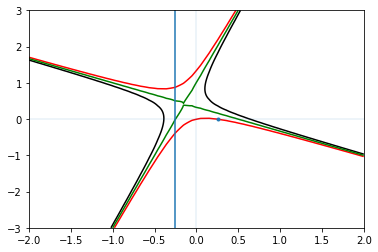
\includegraphics[width=\columnwidth]{./solutions/40/7/figs/A7_4.png}
    \caption{Hyperbola with assymptotes and its conjugate}
    \label{eq:solutions/40/7/Fig :1}
\end{figure}

%
\item What conics do the following equation represents? When possible, find the center and the equation reffered to the center.
\begin{multline}
55x^2 - 120xy + 20y^2 +64x -48y=0
\label{eq:solutions/40/9/eqn1}
\end{multline}
%
\solution
The general equation of second degree can be represented as:
\begin{align}
\vec{X}^T\vec{V}\vec{X} + 2\vec{u}^T\vec{X} + f = 0
\end{align}
The above \ref{eq:solutions/40/9/eqn1} can also be written as:
\begin{align}
\vec{X}^T\myvec{55 & -60\\-60 & 20}\vec{X} + 2\myvec{32 & -24}\vec{X} +0 = 0
\end{align}
So, 
\begin{align}
\vec{V} = \myvec{55 & -60\\-60 & 20}
\end{align}
and 
\begin{align}
\vec{u} = \myvec{32 \\ -24}\\
f=0
\end{align}
Now, 
\begin{align}
\det{\vec{V}} = \mydet{55 & -60\\-60 & 20}\\
\implies \det{\vec{V}} = -2500 <0
\end{align}

As $\det{\vec{V}}<0$, so we can say that the above conic section \ref{eq:solutions/40/9/eqn1} is hyperbola.Now,
\begin{align}
\vec{V}^{-1} =\frac{1}{-2500} \myvec{20 & 60\\60 & 55}
\end{align}
The center of this hyperbola will be:
\begin{align}
\vec{c} = - \vec{V}^{-1} \vec{u}\\
\implies \vec{c} = \frac{1}{2500} \myvec{20 & 60\\60 & 55} \myvec{32 \\ -24}\\
\implies \vec{c} = \myvec{-\frac{8}{25} \\ \frac{6}{25}}\\
\end{align}
 Now the characteristic equation of $\vec{V}$ is obtained as:
\begin{align}
\mydet{\vec{V} - \lambda\vec{I}} =0\\
\implies \mydet{55-\lambda & -60\\-60 & 20-\lambda} = 0\\
\implies \lambda^2 - 75\lambda - 2500=0
\end{align}
The eigen values are given by:
\begin{align}
\lambda_1=100\\
\lambda_2 = -25
\end{align}
The eigen vector $\vec{P}$ is defined as:
\begin{align}
\vec{V}\vec{P} = \lambda \vec{P}\\
\implies (\vec{V} -\lambda\vec{I})\vec{P} = \vec{0}
\end{align}
For $\lambda_1$=100,
\begin{align}
(\vec{V} -\lambda_1\vec{I}) = \myvec{-45 & -60\\-60 & -80}
\end{align}
By row reduction,
\begin{align}
\myvec{-45 & -60\\-60 & -80}\xleftrightarrow[R_1\leftarrow R_1 /(-5)]{R_2\leftarrow R_2/(-5)}\\
\myvec{9 & 12\\12 & 16}\xleftrightarrow[R_1\leftarrow R_1 /3]{R_2\leftarrow R_2/4}\\
\myvec{3 & 4\\3 & 4}\xleftrightarrow[]{R_2\leftarrow R_2-R_1}\myvec{3 & 4\\0 & 0}
\end{align}
So, 
\begin{align}
(\vec{V} -\lambda_1\vec{I})\vec{P_1} = \vec{0}\\
\implies \myvec{3 & 4\\0 & 0} \myvec{v_1\\v_2} = \myvec{0\\0}\\
\implies \vec{P_1} = \myvec{-\frac{4}{3}\\1}
\end{align}
Similarly,
For $\lambda_2$=100,
\begin{align}
(\vec{V} -\lambda_2\vec{I}) = \myvec{80 & -60\\-60 & 45}
\end{align}
By row reduction,
\begin{align}
\myvec{80 & -60\\-60 & 45}\xleftrightarrow[R_1\leftarrow R_1 /5]{R_2\leftarrow R_2/5}\\
\myvec{16 & -12\\-12 & 9}\xleftrightarrow[R_1\leftarrow R_1 /4]{R_2\leftarrow R_2/(-3)}\\
\myvec{4 & -3\\4 & -3}\xleftrightarrow[]{R_2\leftarrow R_2-R_1}\myvec{4 & -3\\0 & 0}
\end{align}
So, 
\begin{align}
(\vec{V} -\lambda_2\vec{I})\vec{P_2} = \vec{0}\\
\implies \myvec{4 & -3\\0 & 0} \myvec{v_1\\v_2} = \myvec{0\\0}\\
\implies \vec{P_2} = \myvec{1\\ \frac{4}{3}}
\end{align}
By eigen decomposition $\vec{V}$ can also be written as:
\begin{align}
\vec{V} = \vec{P}\vec{D}\vec{P}^T
\end{align}
where 
\begin{align}
\vec{P} = \myvec{\vec{P_1} & \vec{P_2}}\\
\vec{D} =\myvec{\lambda_1 & 0\\0 & \lambda_2}
\end{align}
So, 
\begin{align}
\vec{P} = \myvec{-\frac{4}{3} & 1\\1 & \frac{4}{3}}\\
\vec{D} =\myvec{100 & 0\\0 & -25}
\end{align}
and 
\begin{align}
\vec{u}^T\vec{V}^{-1}\vec{u}-f=16>0
\end{align}
So, the axes are:
\begin{align}
a=\sqrt{\frac{\vec{u}^T\vec{V}^{-1}\vec{u}-f}{\lambda_1}} = \frac{2}{5}\\
b=\sqrt{\frac{f-\vec{u}^T\vec{V}^{-1}\vec{u}}{\lambda_2}} = \frac{4}{5}
\end{align}
Now, the equation \ref{eq:solutions/40/9/eqn1} can be written as:
\begin{align}
\vec{y}^T\vec{D}\vec{y}=\vec{u}^T\vec{V}^{-1}\vec{u}-f
\end{align}
where, 
\begin{align}
\vec{y}= \vec{P}^T (\vec{x}-\vec{c})
\end{align}
So, 
\begin{align}
\vec{y}^T\myvec{100 & 0\\0 & -25}\vec{y}=16\\
\implies \vec{y}^T\myvec{100 & 0\\0 & -25}\vec{y}-16=0
\end{align}

\begin{figure}[!ht]
\centering
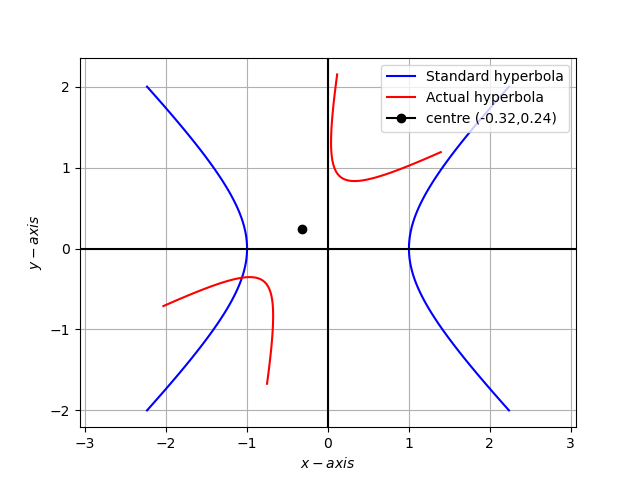
\includegraphics[width=\columnwidth]{./solutions/40/9/figs/hyperbola_2.png}
\caption{Comparison of the Standerd and Actual Hyperbola}
\label{eq:solutions/40/9/fig:hyperbola}
\end{figure}





%
\item  Find the asymptotes of the given hyperbola and also the equation to its conjugate hyperbola
\begin{align}
19x^2 + 24xy+y^2-22x-6y=0 \label{eq:solutions/40/10/1.1}
\end{align}
%
\solution
The general equation of second degree is given by
\begin{align}
ax^2+2bxy+cy^2+2dx+2ey+f=0\label{eq:solutions/40/10/2.1}
\end{align}
and can be expressed as
\begin{align}
\vec{x}^T\vec{V}\vec{x}+2\vec{u}^T\vec{x}+f=0 \label{eq:solutions/40/10/2.2}
\end{align}
where
\begin{align}
\vec{V} &= \vec{V}^T = \myvec{a & b \\ b & c}
\\
\vec{u} &= \myvec{d \\ e}
\intertext{Comparing equations \ref{eq:solutions/40/10/1.1} and \ref{eq:solutions/40/10/2.2} we get}
    \vec{V}=\vec{V}^T&=\myvec{19 & 12 \\ 12 &1}\label{eq:solutions/40/10/2.5}\\
    \vec{u}&=\myvec{-11 \\-3 }\label{eq:solutions/40/10/2.6}\\
    f&=0\label{eq:solutions/40/10/2.7}
\end{align}   
Expanding the Determinant of $\vec{V}$.
\begin{align}
    \Delta_{V} &= \begin{array}{|cc|}
19 &12\\12 & 1
\end{array}<0\label{eq:solutions/40/10/2.8}
\end{align}
Hence from \ref{eq:solutions/40/10/2.8} given
equation represents the hyperbola.\\
The characteristic equation of $\vec{V}$ is obtained by evaluating the determinant 
\begin{align}
       \begin{array}{|c|}
V-\lambda\vec{I}
\end{array}&=0\\
   \begin{array}{|cc|}
19-\lambda & 12 \\ 12 & 1-\lambda
\end{array}&=0\\
    \brak{19-\lambda}\brak{1-\lambda}-144=0\\
    \lambda_{1}=-5,   \lambda_{2}= 25 \label{eq:solutions/40/10/2.12}
\end{align}
The eigenvector $\vec{p}$ is defined as 
\begin{align}
    \vec{V}\vec{p}&=\lambda\vec{p}\\
    \implies (\vec{V}-\lambda\vec{I})\vec{p}&=0\label{eq:solutions/40/10/2.14}
\end{align}
For $\lambda_1=-5$ ,
\begin{align}
    (\vec{V}-\lambda_1\vec{I})=\myvec{19+5 & 12 \\12 & 1+5}
\end{align}
By row reduction , 
\begin{align}
    &\myvec{24 & 12 \\12 & 6}\\
&\xleftrightarrow{R_2\leftarrow 2R_2 -R_1}
    \myvec{24 & 12 \\ 0& 0}\\
        &\xleftrightarrow{R_1\leftarrow \frac{R_1}{12}}
    \myvec{2 & 1 \\ 0& 0}
    \label{eq:solutions/40/10/2.18}
\end{align}
Subsituting equation \ref{eq:solutions/40/10/2.18} in equation \ref{eq:solutions/40/10/2.14} we get
\begin{align}
        &   \myvec{2 & 1 \\ 0& 0}\myvec{u_1 \\ u_2}=\myvec{0 \\ 0}\label{eq:solutions/40/10/2.19}
\end{align}
Where, $\vec{p}=\myvec{u_1\\u_2}$
Let $u_1=t$
\begin{align}
    u_2&=-2t
\end{align}
Eigen vector $\vec{p_1}$ is given by
\begin{align}
    \vec{p_1}&=\myvec{t \\ -2t}
\end{align}
Let $t=1$, we get
\begin{align}
        \vec{p_1}&=\myvec{1 \\-2 }\label{eq:solutions/40/10/2.22}
\end{align}
For $\lambda_2=25$ ,
\begin{align}
    (\vec{V}-\lambda_2\vec{I})=\myvec{19-25 & 12 \\12 & 1-25}
\end{align}
By row reduction , 
\begin{align}
    &\myvec{-6 & 12 \\12 & -24}\\
&\xleftrightarrow{R_2\leftarrow R_2 +2R_1}
    \myvec{-6 & 12 \\ 0& 0}\\
        &\xleftrightarrow{R_1\leftarrow \frac{R_1}{6}}
    \myvec{-1 & 2 \\ 0& 0}
    \label{eq:solutions/40/10/2.26}
\end{align}
Subsituting equation \ref{eq:solutions/40/10/2.26} in equation \ref{eq:solutions/40/10/2.14} we get
\begin{align}
        &   \myvec{-1 & 2 \\ 0& 0}\myvec{v_1 \\ v_2}=\myvec{0 \\ 0}\label{eq:solutions/40/10/2.27}
\end{align}
Where, $\vec{p}=\myvec{v_1\\v_2}$
Let $v_1=t$
\begin{align}
    v_2&=\frac{t}{2}
\end{align}
Eigen vector $\vec{p_2}$ is given by
\begin{align}
    \vec{p_2}&=\myvec{t \\ \frac{t}{2}}
\end{align}
Let $t=1$, we get
\begin{align}
        \vec{p_2}&=\myvec{1 \\\frac{1 }{2}}\label{eq:solutions/40/10/2.30}
\end{align}
By eigen decompostion $\vec{V}$ can be represented by
\begin{align}
    \vec{V}&=\vec{P}\vec{D}\vec{P}^T\label{eq:solutions/40/10/2.31}
\end{align}
where 
\begin{align}
        \vec{P}&=\myvec{\vec{p_1} & \vec{p_2}}\label{eq:solutions/40/10/2.32}\\
    \vec{D}&=\myvec{\lambda_1 & 0 \\0 & \lambda_2}\label{eq:solutions/40/10/2.33}
\end{align}

Substituting equations \ref{eq:solutions/40/10/2.22}, \ref{eq:solutions/40/10/2.30} in equation \ref{eq:solutions/40/10/2.32} we get 
\begin{align}
    \vec{P}&=\myvec{1 & 1 \\-2 & \frac{1}{2}}\label{eq:solutions/40/10/2.34}
\end{align}
Substituting equation \ref{eq:solutions/40/10/2.12} in \ref{eq:solutions/40/10/2.33} we get
\begin{align}
       \vec{D}&=\myvec{-5 & 0\\0 & 25}\label{eq:solutions/40/10/2.35}
\end{align}
Equation of a hyperbola and the combined equation of the Asymptotes differ only in the constant term.
\begin{align}
 19x^2 + 24xy+y^2-22x-6y+K=0   \label{eq:solutions/40/10/2.36}
\end{align}
The above equation can be expressed in the form 
\begin{align}
\vec{x}^T\vec{V}\vec{x}+2\vec{u}^T\vec{x}+f&=0 \label{eq:solutions/40/10/2.37}
\intertext{Comparing equation we get}
    \vec{V}=\vec{V}^T&=\myvec{19 & 12 \\ 12 &1}\label{eq:solutions/40/10/2.38}\\
    \vec{u}&=\myvec{-11 \\-3 }\label{eq:solutions/40/10/2.39}\\
    f&=K\label{eq:solutions/40/10/2.40}
\end{align}
\begin{align}
\Delta&=\begin{array}{|ccc|}19 & 12 & -11\\ 12& 1 & -3\\ -11 & -3 & K
\end{array}
\end{align}
Since the equations represent pair of straight lines, equating the determinant to zero, we can get the value of K
\begin{align}
\implies K=4 \label{eq:solutions/40/10/2.42}
\end{align}
Let $(\alpha,\beta)$ be their point of intersection, then
\begin{equation}\label{eq:solutions/40/10/2.43}
	\myvec{ a & b\\ b & c}\myvec{\alpha \\ \beta} = \myvec{-d \\ -e}
\end{equation}
Substituting the values, we obtain,
\begin{align}
\myvec{19 & 12 \\ 12 &1}\myvec{\alpha \\ \beta} = \myvec{11 \\ 3}\\
\text{We get, } \alpha =  \frac{1}{5} , \beta = \frac{3}{5}
\end{align}

Using Affine transformation and Spectral decomposition, we get
\begin{align}
X^\prime = \pm \sqrt{-\frac{\lambda_2}{\lambda_1}}Y^\prime\\
\text{where } X^\prime = Xu_1 + Yu_2 \\
Y^\prime = Xv_1 + Yv_2\\
X = x-\alpha \text{ and } Y = y - \beta
\end{align}
Therefore, 
\begin{multline}
	u_1(x-\alpha) + u_2(y-\beta) = \\ \pm \sqrt{-\frac{\lambda_2}{\lambda_1}}(v_1(x-\alpha) + v_2(y-\beta))  
%\label{eq:solutions/40/10/2.57}
\end{multline}
Substituting values, we get 
\begin{multline}
	(x-\frac{1}{5})-2(y-\frac{3}{5}) = \\ \pm \sqrt{\frac{25}{5}}(x-\frac{1}{5})+\frac{1}{2}(y-\frac{3}{5}) 
\end{multline}
Simplifying above equation
\begin{align}
	8x+ 9y - 7 = 0 \\
	12x + y + 7 = 0\\
	\implies (8x+ 9y - 7 )(12x + y + 7) = 0
\end{align}
Thus the equation of lines are
\begin{align}
	\myvec{8 & 9}\vec{x} = 7 \\
	\myvec{12 & 1}\vec{x} = -7 
\end{align}

 The Equation of Conjugate hyperbola is given by:\\
\\
2(Equation of Asymptotes)- Equation of hyperbola.\\
\\
From Eq \ref{eq:solutions/40/10/1.1} and \ref{eq:solutions/40/10/2.36}, we obtain equation of Conjugate hyperbola as:-
\begin{align}
19x^2 + 24xy+y^2-22x-6y+8=0  \label{eq:solutions/40/10/2.57}
\end{align}
The general equation of second degree is given by
\begin{align}
ax^2+2bxy+cy^2+2dx+2ey+f=0\label{eq:solutions/40/10/2.59}
\end{align}
comparing equation \ref{eq:solutions/40/10/2.57} with the general equation of second degree given at \ref{eq:solutions/40/10/2.59}, it can be expressed as
\begin{align}
\vec{x}^T\vec{V}\vec{x}+2\vec{u}^T\vec{x}+f=0 \label{eq:solutions/40/10/2.58}
\end{align}
where
\begin{align}
\vec{V} &= \vec{V}^T = \myvec{a & b \\ b & c}
\\
\vec{u} &= \myvec{d\\ e}
\intertext{Comparing equations \ref{eq:solutions/40/10/2.57} and \ref{eq:solutions/40/10/2.58} we get}
    \vec{V}=\vec{V}^T&=\myvec{19 & 12 \\ 12 &1}\\
    \vec{u}&=\myvec{-11 \\-3 }\\
    f&=8
\end{align}   
Therefore, the equation of the conjugate hyperbola is as given below:-
\begin{align}
\vec{x}^T\myvec{19 & 12 \\12 & 1}\vec{x} +2\myvec{-11 & -3} \vec{x}&+8= 0 \label{eq:solutions/40/10/2.66}
\end{align}

\begin{figure}[h]
    \centering
    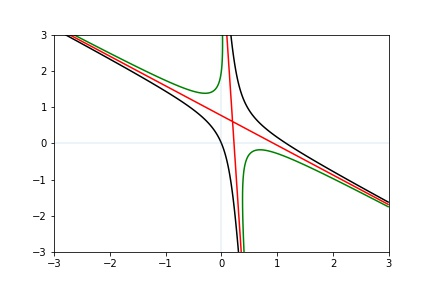
\includegraphics[width=\columnwidth]{./solutions/40/10/hyperbola.jpg}
    \caption{Hyperbola, Conjugate Hyperbola and Asymptotes}
    \label{eq:solutions/40/10/Fig :1}
\end{figure}

\end{enumerate}



\subsection{41}
\renewcommand{\theequation}{\theenumi}
\renewcommand{\thefigure}{\theenumi}
\begin{enumerate}[label=\thesubsection.\arabic*.,ref=\thesubsection.\theenumi]
\numberwithin{equation}{enumi}
\numberwithin{figure}{enumi}
%
\item Trace the parabola:
\begin{align}
	(x-4y)^2=51y
\end{align}
%
\solution
Expanding the given equation, we have,
\begin{align}
    x^2 -8xy +16y^2 -51y =0 \label{eq:solutions/41/1/eq:1}
\end{align}
The general equation of second degree is given by
\begin{align}
	ax^2+2bxy+cy^2+2dx+2ey+f=0 \label{eq:solutions/41/1/gen_eq}
\end{align}
and can be expressed as
\begin{align}
	\vec{x}^T\vec{V}\vec{x}+2\vec{u}^T\vec{x}+f=0 \label{eq:solutions/41/1/conic_eq}
\end{align}
where
\begin{align}
	\vec{V} &= \vec{V}^T = \myvec{a & b \\ b & c}
	\\
	\vec{u}^T &= \myvec{d & e}
\end{align}
From equation \eqref{eq:solutions/41/1/eq:1} , we get
\begin{align}
	\vec{V} &= \myvec{1 & -4\\-4 & 16}\label{eq:solutions/41/1/eq:2}\\
	\vec{u} &= \myvec{0\\-\frac{51}{2}}\label{eq:solutions/41/1/eq:3}\\ 
	f &= 0 \label{eq:solutions/41/1/eq:4}
\end{align}
Expanding the determinant of $\vec{V}$ we observe, 
\begin{align}
	\mydet{1 & -4\\-4 & 16} = 0
\end{align}
Therefore, \eqref{eq:solutions/41/1/eq:1} is a parabola.

The characteristic equation of $\vec{V}$ is given as follows,
\begin{align}
		\mydet{\lambda\vec{I}-\vec{V}} = \mydet{\lambda-1&4\\ 4&\lambda-16} &= 0\\
		\implies \lambda^2-17\lambda &= 0\label{eq:solutions/41/1/eq:5}
\end{align}
The eigenvalues are given by
\begin{align}
		\lambda_1=0, \lambda_2=17\label{eq:solutions/41/1/eq:6}    
\end{align}
For $\lambda_1 = 0$, the eigen vector $\vec{p}$ is given by 
\begin{align}
		\vec{V}\vec{p} = 0
\end{align}

Row reducing $\vec{V}$ 
\begin{align}
		\myvec{1&-4\\-4&16}\xleftrightarrow[R_2=R_2+R_1]{R_2=R_2/4}\myvec{1&-4\\0&0}\\
		\implies\vec{p}_1=\frac{1}{\sqrt{17}}\myvec{-4\\-1} \label{eq:solutions/41/1/eq:7}
\end{align}
Similarly, 
\begin{align}
		\vec{p}_2=\frac{1}{\sqrt{17}}\myvec{-1\\4} \label{eq:solutions/41/1/eq:8}
\end{align}

Thus,
\begin{align}
		\vec{P}&=\myvec{\vec{p_1}&\vec{p_2}}=\frac{1}{\sqrt{17}} \myvec{-4 & -1\\ -1 & 4} 
\end{align}
The equation of the parabola is:
\begin{align}
		\vec{y^T}\vec{D}\vec{y}&=-2\eta\myvec{1&0}\vec{y}
\end{align}
where
\begin{align}
		\eta=\vec{u}^T\vec{p_1}=\frac{51}{2\sqrt{17}}
\end{align}
and focal length of the parabola is given by 
\begin{align}
	\frac{\abs{2\vec{u}^T\vec{p_1}}}{\lambda_2}	= \frac{3}{\sqrt{17}}
\end{align}

Now,
\begin{align}
		\myvec{\vec{u^T}+\eta\vec{p_1^T} \\ \vec{V}}\vec{c}=
		\myvec{-f \\ \eta\vec{p_1}-\vec{u}} \label{eq:solutions/41/1/eq:9}
\end{align}
using equations \eqref{eq:solutions/41/1/eq:2}, \eqref{eq:solutions/41/1/eq:3} and \eqref{eq:solutions/41/1/eq:9}
\begin{align}
	\myvec{-6& -27 \\ 1 & -4 \\  -4 & 16 }\vec{c}=\myvec{0 \\ -6\\ 24} 
\end{align}

Forming the augmented matrix and row reducing it:
\begin{align}
		\myvec{-6 & -27 & 0\\1 & -4 & -6 \\-4 & 16 & 24}\\
		\xleftrightarrow[]{R_3\leftarrow R_3+ 4R_2} 
		\myvec{-6 & -27 & 0\\1 & -4 & -6 \\0 & 0 &0 }\\
		\xleftrightarrow[]{R_1\leftarrow R_1/(-6)} 
		\myvec{1 & 9/2 & 0\\1 & -4 & -6\\0 & 0 &0 }\\
		\xleftrightarrow[]{R_2\leftarrow R_2-R_1} 
		\myvec{1 & 9/2 & 0\\0 & -17/2 & -6 \\0 & 0 &0 }\\
		\xleftrightarrow[]{R_2\leftarrow (-\frac{2}{17})R_2}
		\myvec{1 & 9/2 & 0\\0 & 1 & 12/17\\0 & 0 &0}\\ 
		\xleftrightarrow[]{R_1\leftarrow R_1 -(\frac{9}{2})R_2}
		\myvec{1 & 0 & -54/17\\0 & 1 & 12/17 \\0 & 0 &0}
\end{align}

Thus the vertex is:
\begin{align}
	&\vec{c}= \myvec{-\frac{54}{17}\\ \frac{12}{17}} \\
	&\approx \myvec{-3.18\\ 0.71}
\end{align}

\begin{figure}[!htbp]
	\centering
	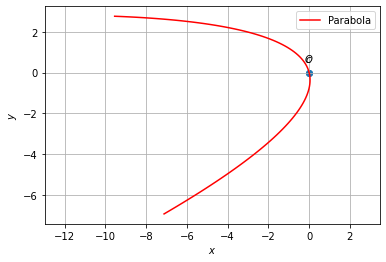
\includegraphics[width =\columnwidth]{solutions/41/1/parabola plot.png}
	\caption{Parabola }
	\label{eq:solutions/41/1/fig:1}
\end{figure}	



%
\item 	Trace the curve 
	\begin{align}
	\left(x-y\right)^2 = x+y+1
	\label{eq:solutions/41/2/eq0}
	\end{align}
%
\solution
	
	We have given equation as :
	\begin{align}
\left(x-y\right)^2 = x+y+1
\end{align}	
\begin{align}
\implies x^2  -2xy + y^2 -x - y -1 = 0
\label{eq:solutions/41/2/eq1}
\end{align}
The general equation of second degree is given by
\begin{align}
ax^2+2bxy+cy^2+2dx+2ey+f=0 \label{eq:solutions/41/2/eq2}
\end{align}
and can be expressed as
\begin{align}
\vec{x}^T\vec{V}\vec{x}+2\vec{u}^T\vec{x}+f=0 \label{eq:solutions/41/2/eq3}
\end{align}
where
\begin{align}
\vec{V} &= \vec{V}^T = \myvec{a & b \\ b & c}
\\
\vec{u}^T &= \myvec{d & e}
\end{align}

Comparing \eqref{eq:solutions/41/2/eq1} with \eqref{eq:solutions/41/2/eq2}, we get

\begin{align}
\vec{V} &= \vec{V}^T = \myvec{ 1 &  -1 \\ -1 & 1 }
\\
\vec{u}^T &= \myvec{-\frac{1}{2} & - \frac{1}{2}}
\\
f &= -1
\end{align}


Expanding the determinant of V we observe,
\begin{align}
\abs{\vec{V}} = \mydet{1 & -1 \\ -1 & 1} = 0 \label{eq:solutions/41/2/eq10}
\end{align}
Also
\begin{align}
\mydet{\vec{V} & \vec{u} \\ \vec{u}^T & f} = 
\mydet{
1 & -1 & -\frac{1}{2} \\ 
-1 & 1 & -\frac{1}{2} \\ 	
-\frac{1}{2} & -\frac{1}{2} & -1}
\neq 0
\label{eq:solutions/41/2/eq11}
\end{align}

Hence from \eqref{eq:solutions/41/2/eq10} and \eqref{eq:solutions/41/2/eq11} we conclude
that given equation is an parabola.The characteristic equation of $\vec{V}$ is given as
follows,


\begin{align}
\mydet{\lambda \vec{I}-\vec{V}} = \mydet{\lambda -1 & -1 \\ -1 & \lambda - 1} &= 0
\\
\implies \left(\lambda - 1 \right)^2 -1 &= 0
\label{eq:solutions/41/2/eq12}
\end{align}
The eigenvalues are the roots of \eqref{eq:solutions/41/2/eq12} given by
\begin{align}
\lambda_1 = 0, \lambda_2 = 2
\label{eq:solutions/41/2/eq13}
\end{align}
The eigenvector $\vec{p}$ is defined as:
\begin{align}
\vec{V} \vec{p}&= \lambda \vec{p}
\\
\implies \brak{\lambda\vec{I}-\vec{V}}\vec{p} &=0
\end{align}
where $\lambda$ is the eigenvalue.  For $\lambda_1$ = 0,
\begin{align}
\vec{V} \vec{p}&=0
\end{align}
Row reducing $\vec{V}$ yields,
\begin{align}
 \myvec{ 1 & -1 \\ -1 & 1} 
\xleftrightarrow{R_2\leftarrow R_2+R_1} 
\myvec{
	1 &  -1 \\ 0 & 0 
} 
\label{eq:solutions/41/2/eq18}
\end{align}

  Similarly, the eigenvector corresponding to $\lambda_2$ can be obtained as
  
  \begin{align}
  \brak{\lambda_2\vec{I}-\vec{V}}
  = \myvec{ 1 & 1 \\ 1 & 1} 
  \xleftrightarrow{R_2\leftarrow R_2 - R_1}
  \myvec{
  	1 & 1   \\ 0 & 0 
  }
  \label{eq:solutions/41/2/eq19}
  \end{align}
  
  
  

It is easy to verify that 
\begin{align}
\vec{V} &= \vec{P}\vec{D}\vec{P}^{-1}=\vec{P}\vec{D}\vec{P}^T \quad \because \vec{P}^{-1} = \vec{P}^{T} \label{eq:solutions/41/2/eq:solutions/41/ex1/ellipse_spectrum_eq}
\\
\text{or, } \vec{D} &= \vec{P}^T\vec{V}\vec{P}
\end{align}


From equation \eqref{eq:solutions/41/2/eq18} and \eqref{eq:solutions/41/2/eq19}, we have
\begin{align}
\vec{p_1} =  \frac{1}{\sqrt{2}} \myvec{1 \\ 1} 
\text{and},  \vec{p_2} =  \frac{1}{\sqrt{2}} \myvec{1 \\ -1} 
\end{align}
Thus, the eigenvector rotation matrix and the
eigenvalue matrix are 
\begin{align}
\vec{P} &= \frac{1}{\sqrt{2}} \myvec{ \vec{p_1} & \vec{p_2}} = \frac{1}{\sqrt{2}} \myvec{ 1 & 1 \\ 1 & -1} \\
 \vec{D} &= \myvec{0 & 0 \\ 0 & 2} 
\end{align}

\begin{figure}[htb!]	
	\centering	
	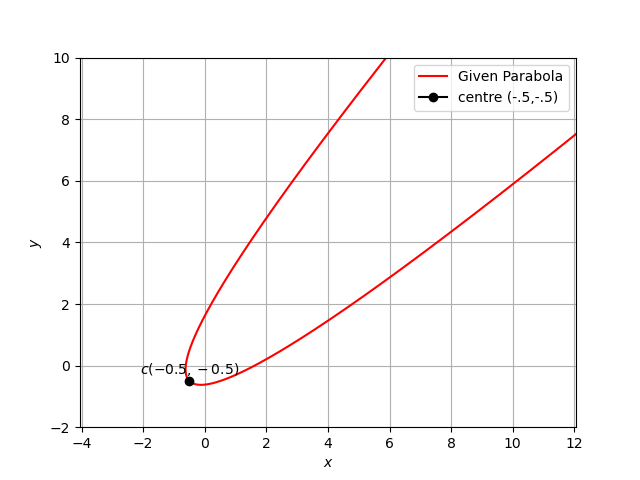
\includegraphics[width=\columnwidth]{./solutions/41/2/parabola.png}	
	\caption{Parabola with the center c}
	\label{eq:solutions/41/2/fig1}	
\end{figure}

The focal length of the parabola is
given by
\begin{align}
\frac{\mydet{2{\vec{u}}^T\vec{p_1}}}{\lambda_2 } = \frac{\sqrt{2}}{2} = \sqrt{2}
\end{align}
and its equation is
\begin{align}
\vec{y}^T\vec{D}\vec{y} = -2 \eta\myvec{1 & 0 }\vec{y}
\end{align}
where,
\begin{align}
\eta = \vec{u}^T\vec{p_1} = - \frac{1}{\sqrt{2}}
\end{align}

\begin{align}
\myvec{\vec{u}^T + \eta\vec{p_1}^T \\ \vec{V}}\vec{c} = \myvec{-f \\ \eta\vec{p_1} - \vec{u}} 
\end{align}
\begin{align}
\implies \myvec{ -1 & -1   \\ 1 & -1 \\ -1 & 1 }\vec{c} = \myvec{1 \\ 0 \\ 0}
\end{align}
Forming the augmented matrix and row reducing
it:


%\begin{align}
%\myvec{-1  &  -1 &  1 \\   1 & -1 &  1 \\  -1 & 1 & 0}  \label{eq:solutions/41/2/2.30}
%\end{align}

\begin{align}
\myvec{-1  &  -1 &  1 \\   1 & -1 &  1 \\  -1 & 1 & 0}  \label{eq:solutions/41/2/2.30}
\xleftrightarrow[]{R_2 \leftarrow R_2+R_1  }
%
\myvec{
-1 & -1 & 1 \\ 0 & -2 & 1 \\ -1 & 1 & 0  
} 
\xleftrightarrow[R_1 \leftarrow -1R_1] {R_3 \leftarrow  R_3 - R_1}  \nonumber  \\
%
\myvec{
1 & 1 & -1 \\ 0 & -2 & 1 \\ 0 & 2 & -1 
}
\xleftrightarrow[]{R_3 \leftarrow R_3 +R_2 } 
%	
\myvec{
1 & 1 & -1 \\ 0 & -2 & 1 \\ 0 & 0 & 0 
} \nonumber   \\
\xleftrightarrow[R_1 \leftarrow R_1 -R_2]{R_1 \leftarrow \frac{R_1}{-2}} 
\myvec{
1 & 0 & -\frac{1}{2} \\ 0 & 1 & - \frac{1}{2} \\ 0 & 0 & 0
}
\end{align}
So,
\begin{align}
\vec{c} = \myvec{ -\frac{1}{2} \\ -\frac{1}{2}  } \label{eq:solutions/41/2/2.31}
\end{align}







%
\item Trace the parabola
\begin{align}
    (4x+3y+15)^2=5(3x-4y)
\end{align}
%
\solution
%
The given equation can be rewritten as
\begin{align}\label{eq:solutions/41/4/eq:quadraticparabola}
    16x^2+24xy+9y^2+105x+110y+225 = 0
\end{align}
Comparing this to the standard equation,
%\vec{x}^T\vec{V}\vec{x}+2\vec{u}^T\vec{x}+f = 0
\begin{align}
    \vec{V} = \vec{V}^T = \myvec{16 & 12\\12 & 9}, \quad \vec{u} = \myvec{\frac{105}{2} \\ 55}, \quad f = 225 \label{eq:solutions/41/4/eq:Vufvals}
\end{align}
The characteristic equation of $\vec{V}$ is given as
\begin{align}
    \mydet{\lambda\vec{I}-\vec{V}} = 0\\
    \implies \mydet{\lambda-16 & -12 \\ -12 & \lambda-9} = 0\\
    \implies \lambda^2 -25\lambda = 0 \label{eq:solutions/41/4/eq:lambdaeq}
\end{align}
The eigenvalues are the roots of the equation \eqref{eq:solutions/41/4/eq:lambdaeq}, which are as follows :
\begin{align}
    \lambda_1 = 0, \quad \lambda_2 = 25 \label{eq:solutions/41/4/eq:eigenval}
\end{align}
The eigen vector $\vec{p}$ is defined as, 
\begin{align}
    \vec{V}\vec{p} &= \lambda\vec{p}\\
    \implies(\lambda\vec{I}-\vec{V})\vec{p}&=0
\end{align}
For $\lambda_1=0$
\begin{align}
    (\lambda_1\vec{I}-\vec{V}) = \myvec{-16 & -12\\-12 & -9}\xleftrightarrow[R_2\leftarrow R_2-3R_1]{R_1\leftarrow \frac{1}{4}R_1}\myvec{-4 & -3\\0 & 0}
\end{align}
\begin{align}
    \implies\vec{p_1}&=\frac{1}{5}\myvec{-3\\4}\label{eq:solutions/41/4/eq:p1val}
\end{align}
For $\lambda_2=25$
\begin{align}
    (\lambda_2\vec{I}-\vec{V}) = \myvec{9 & -12\\-12 & 16}\xleftrightarrow[R_2\leftarrow R_2+4R_1]{R_1\leftarrow \frac{1}{3}R_1}\myvec{3 & -4\\0 & 0}
\end{align}
\begin{align}
    \implies\vec{p_2}=\frac{1}{5}\myvec{4\\3}\label{eq:solutions/41/4/eq:p2val}
\end{align}
So, using Eigenvalue decomposition, $\vec{P}^T\vec{V}\vec{P}=\vec{D}$, where
\begin{align}
    \vec{P} = \frac{1}{5}\myvec{-3 & 4\\4 & 3}\\
    \vec{D} = \myvec{\lambda_1 & 0\\0 & \lambda_2} = \myvec{0 & 0\\ 0 & 25}
\end{align}
Then, for the parabola
\begin{align}
    \text{focal length} = \abs{\frac{2\eta}{\lambda_2}} \label{eq:solutions/41/4/eq:focallen}\\
    \eta = \vec{p}_1^T\vec{u} = \frac{25}{2}\label{eq:solutions/41/4/eq:etaval}\\
    \intertext{Substituting values from \eqref{eq:solutions/41/4/eq:etaval} and \eqref{eq:solutions/41/4/eq:eigenval} in \eqref{eq:solutions/41/4/eq:focallen}, we get}
    \text{focal length} = 1
\end{align}
The standard equation of the parabola is given by
\begin{align}
    \vec{y}^T\vec{D}\vec{y} = -2\eta\myvec{1 & 0}\vec{y}
\end{align}
And the vertex $\vec{c}$ is given by
\begin{align}
    \myvec{\vec{u}^T + \eta\vec{p}_1^T \\ \vec{V}}\vec{c} = \myvec{-f \\ \eta\vec{p}_1 - \vec{u}} \label{eq:solutions/41/4/eq:c}
\end{align}
Substituting values from \eqref{eq:solutions/41/4/eq:Vufvals},\eqref{eq:solutions/41/4/eq:etaval},\eqref{eq:solutions/41/4/eq:p1val} in \eqref{eq:solutions/41/4/eq:c},
\begin{align}
    \myvec{45 & 65\\16 & 12\\12 & 9}\vec{c} = \myvec{-225\\-60\\-45}
\end{align}
To find $\vec{c}$, performing row reduction on the augmented matrix as follows:
\begin{align}
    \myvec{45 & 65 & -225\\16 & 12 & -60\\12 & 9 & -45}\xleftrightarrow[R_1\leftarrow \frac{1}{45}R_1]{R_3\leftarrow R_3-\frac{3}{4}R_2}\myvec{1 & \frac{13}{9} & -5\\16 & 12 & -60\\0&0&0}\\
    \xleftrightarrow{R_2\leftarrow R_2-16R_1}\myvec{1 & \frac{13}{9} & -5\\0 & \frac{-100}{9} & 20\\0&0&0}\\\xleftrightarrow{R_2\leftarrow \frac{-9}{100}R_2}\myvec{1 & \frac{13}{9} & -5\\0 & 1 & \frac{-9}{5}\\0&0&0}\\\xleftrightarrow{R_1\leftarrow R_1-\frac{13}{9}R_2}\myvec{1 & 0 & \frac{-12}{5}\\0 & 1 & \frac{-9}{5}\\0&0&0}
\end{align}
Thus,
\begin{align}
    \vec{c} = \myvec{\frac{-12}{5}\\\frac{-9}{5}} = \myvec{-2.4 \\ -1.8}
\end{align}
\begin{figure}[h!]
    \centering
    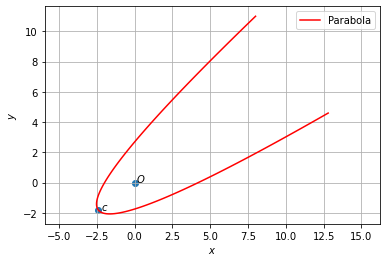
\includegraphics[width=\columnwidth]{./solutions/41/4/assignment5parabola.png}
    \caption{Parabola with vertex c}
    \label{eq:solutions/41/4/fig:fig1}
\end{figure}

%
\item Trace the parabola
\begin{align}\nonumber
    16x^2+24xy+9y^2-5x-10y+1 = 0
\end{align}
%
\solution
Compare the given equation with the standard form
\begin{align}\label{eq:solutions/41/5/eq:1}
    ax^2+2bxy+cy^2+2dx+2ey+f = 0
\end{align}
Write the values Of V and u as follows
\begin{align}
    \vec{V} = \vec{V}^T = \myvec{16 & 12\\12 & 9} \quad
    \vec{u} =\myvec{-\frac{5}{2} \\ -5} \quad
     f = 1 \label{eq:solutions/41/5/eq:2}
\end{align}
The characteristic equation of $\vec{V}$ is given as
\begin{align}
    \mydet{\lambda\vec{I}-\vec{V}} = 0\\
    \implies \mydet{\lambda-16 & -12 \\ -12 & \lambda-9} = 0\\
    \implies \lambda^2 -25\lambda = 0 \label{eq:solutions/41/5/eq:3}
\end{align}
The eigenvalues are the roots of the equation \eqref{eq:solutions/41/5/eq:3} are
\begin{align}
    \lambda_{1} = 0, \quad \lambda_{2} = 25 \label{eq:solutions/41/5/eq:4}
\end{align}
The eigen vector $\vec{p}$ is defined as, 
\begin{align}
    \vec{V}\vec{p} &= \lambda\vec{p}\\
    \implies(\lambda\vec{I}-\vec{V})\vec{p}&=0
\end{align}
For $\lambda_1=0$
\begin{align}
    (\lambda_1\vec{I}-\vec{V}) = \myvec{-16 & -12\\-12 & -9}\xleftrightarrow[R_2\leftarrow R_2-3R_1]{R_1\leftarrow \frac{1}{4}R_1}\myvec{-4 & -3\\0 & 0}
\end{align}
\begin{align}
    \implies\vec{p_1}&=\frac{1}{5}\myvec{-3\\4}\label{eq:solutions/41/5/eq:p1val}
\end{align}
For $\lambda_2=25$
\begin{align}
    (\lambda_2\vec{I}-\vec{V}) = \myvec{9 & -12\\-12 & 16}\xleftrightarrow[R_2\leftarrow R_2+4R_1]{R_1\leftarrow \frac{1}{3}R_1}\myvec{3 & -4\\0 & 0}
\end{align}
\begin{align}
    \implies\vec{p_2}=\frac{1}{5}\myvec{4\\3}\label{eq:solutions/41/5/eq:p2val}
\end{align}
Use Eigenvalue decomposition, $\vec{P}^T\vec{V}\vec{P}=\vec{D}$, where
\begin{align}
    \vec{P} = \frac{1}{5}\myvec{-3 & 4\\4 & 3}\\
    \vec{D} = \myvec{\lambda_1 & 0\\0 & \lambda_2} = \myvec{0 & 0\\ 0 & 25}
\end{align}
Focal length of the parabola is given as
\begin{align}
    \text{focal length} = \abs{\frac{2\eta}{\lambda_2}}\label{eq:solutions/41/5/eq:fl}\\
    \eta = \vec{p}_1^T\vec{u} = -\frac{5}{2}\label{eq:solutions/41/5/eq:eta}\\
    \intertext{Substituting values from \eqref{eq:solutions/41/5/eq:eta} and \eqref{eq:solutions/41/5/eq:4} in \eqref{eq:solutions/41/5/eq:fl}, we get}
    \text{focal length} = \frac{1}{5}
\end{align}
The standard equation of the parabola is given by
\begin{align}
    \vec{y}^T\vec{D}\vec{y} = -2\eta\myvec{1 & 0}\vec{y}
\end{align}
And the vertex $\vec{c}$ is given by
\begin{align}
    \myvec{\vec{u}^T + \eta\vec{p}_1^T \\ \vec{V}}\vec{c} = \myvec{-f \\ \eta\vec{p}_1 - \vec{u}} \label{eq:solutions/41/5/eq:c}
\end{align}
Substituting values from \eqref{eq:solutions/41/5/eq:2},\eqref{eq:solutions/41/5/eq:eta},\eqref{eq:solutions/41/5/eq:p1val} in \eqref{eq:solutions/41/5/eq:c},
\begin{align}
    \myvec{-1 & -7\\16 & 12\\12 & 9}\vec{c} = \myvec{-1\\4\\3}
\end{align}
To find $\vec{c}$, performing row reduction on the augmented matrix as follows:
\begin{align}
    \myvec{-1 & -7 & -1\\16 & 12 & 4\\12 & 9 & 3}\xleftrightarrow[R_1\leftarrow -R_1]{R_3\leftarrow R_3-\frac{3}{4}R_2}\myvec{1 & 7 & 1\\16 & 12 & 4\\0&0&0}\\
    \xleftrightarrow{R_2\leftarrow R_2-16R_1}\myvec{1 & 7 & 1\\0 & -100 & -12\\0&0&0}\\\xleftrightarrow{R_2\leftarrow \frac{-1}{100}R_2}\myvec{1 & 7 & 1\\0 & 1 & \frac{3}{25}\\0&0&0}\\\xleftrightarrow{R_1\leftarrow R_1-7R_2}\myvec{1 & 0 & \frac{4}{25}\\0 & 1 & \frac{3}{25}\\0&0&0}
\end{align}
Thus,
\begin{align}
    \vec{c} = \myvec{\frac{4}{25}\\\frac{3}{25}} %= \myvec{-2.4 \\ -1.8}
\end{align}
\begin{figure}[h!]
    \centering
    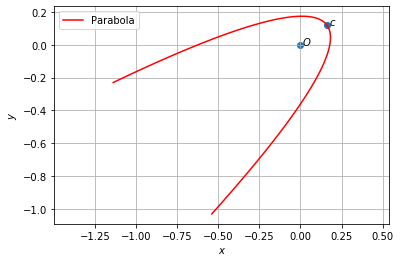
\includegraphics[width=\columnwidth]{./solutions/41/5/A6.png}
    \caption{Parabola with vertex c}
    \label{eq:solutions/41/5/fig:fig1}
\end{figure}

%
\item Trace the parabola
\begin{align}
  9x^2+24xy+16y^2-4y-x+7=0 \label{eq:solutions/41/6/eq:prob}
\end{align}
%
\solution
The general second degree equation can be expressed as
\begin{align}
    \vec{x}^T\vec{V}\vec{x}+2\vec{u}^T\vec{x}+f = 0\label{eq:solutions/41/6/eq:gen}
\end{align}
Comparing \eqref{eq:solutions/41/6/eq:prob} and \eqref{eq:solutions/41/6/eq:gen} we get
\begin{align}
    \vec{V}&=\myvec{9 & 12 \\ 12 & 16}\label{eq:solutions/41/6/eq:V}\\
    \vec{u}&=\myvec{\frac{-1}{2} \\ -2}\label{eq:solutions/41/6/eq:u}\\
    f&=7\label{eq:solutions/41/6/eq:f}
\end{align}
The characteristic equation of $\vec{V}$ is given as
\begin{align}
    \mydet{\vec{V}-\lambda\vec{I}}&=0\\
    \implies\mydet{9-\lambda & 12\\12&16-\lambda}&=0\\
    \implies\lambda^2-25\lambda&=0\label{eq:solutions/41/6/eq:characteristic}
\end{align}
The roots of $\eqref{eq:solutions/41/6/eq:characteristic}$ are eigenvalue of $\vec{V}$ and are given by
\begin{align*}
    \lambda_1=0,\lambda_2=25
\end{align*}
The eigenvector $\vec{p}$ is defined as
\begin{align}
    \vec{V}\vec{p}&=\lambda\vec{p}\\
    \implies(\vec{V}-\lambda\vec{I})\vec{p}&=0\label{eq:solutions/41/6/eq:eigenval}
\end{align}
For $\lambda_1=0$
\begin{align}
    &(\vec{V}-\lambda\vec{I})=\myvec{9&12\\12&16}\xleftrightarrow{R_2=R_2-\frac{4}{3}R_1}\myvec{9&12\\0&0}\label{eq:solutions/41/6/eq:lambda1}
\end{align}
Substituting equation \eqref{eq:solutions/41/6/eq:lambda1} in equation \eqref{eq:solutions/41/6/eq:eigenval} and upon normalization we get
\begin{align}
    \vec{p_1} = \frac{1}{5}\myvec{-4\\3}\label{eq:solutions/41/6/eq:p1}
\end{align}
For $\lambda_2=25$
\begin{align}
    &(\vec{V}-\lambda\vec{I})=\myvec{-16&12\\12&-9}\xleftrightarrow{R_2=R_2+\frac{3}{4}R_1}\myvec{-16&12\\0&0}\label{eq:solutions/41/6/eq:lambda2}
\end{align}
Substituting equation \eqref{eq:solutions/41/6/eq:lambda2} in equation \eqref{eq:solutions/41/6/eq:eigenval} and upon normalization we get
\begin{align}
    \vec{p_2} = \frac{1}{5}\myvec{3\\4}
\end{align}
The matrix $\vec{P}$ and $\vec{D}$ are
\begin{align}
    \vec{P} = \myvec{\vec{p1}&\vec{p2}}=\frac{1}{5}\myvec{-4&3\\3&4}
\end{align}
and
\begin{align}
    \vec{D} = \myvec{\lambda_1&0\\0&\lambda_2} = \myvec{0&0\\0&25}
\end{align}
Then for the parabola
\begin{align}
    \eta = 2\vec{p_1}^T\vec{u}&=-\frac{8}{5}\label{eq:solutions/41/6/eq:eta}\\
    focal\;length =\mydet{\frac{\eta}{\lambda_2}}&=\frac{8}{125}
\end{align}
For parabola $\mydet{\vec{V}}$ = 0,so equation \eqref{eq:solutions/41/6/eq:gen} can be written as
\begin{align}
    \vec{y}^T\vec{D}\vec{y}=-\eta\myvec{1&0}\vec{y}
\end{align}
And the vertex $\vec{c}$ is given by
\begin{align}
    \myvec{\vec{u}^T+\frac{\eta}{2}\vec{p_1}^T\\\vec{V}}\vec{c}=\myvec{-f\\\frac{\eta}{2}\vec{p_1}-\vec{u}}\label{eq:solutions/41/6/eq:c}
\end{align}
Substituting values from \eqref{eq:solutions/41/6/eq:V}, \eqref{eq:solutions/41/6/eq:u}, \eqref{eq:solutions/41/6/eq:f}, \eqref{eq:solutions/41/6/eq:p1}, \eqref{eq:solutions/41/6/eq:eta} in \eqref{eq:solutions/41/6/eq:c}
\begin{align}
    \myvec{\frac{7}{50}&-\frac{124}{50}\\9&12\\12&16}\vec{c}=\myvec{-7\\\frac{57}{50}\\\frac{76}{50}}
\end{align}
To find $\vec{c}$,performing row reduction in augmented matrix as follows
\begin{align*}
    \myvec{\frac{7}{50}&-\frac{124}{50}&-7\\9&12&\frac{57}{50}\\12&16&\frac{76}{50}}\xleftrightarrow[R_1\leftarrow \frac{50}{7}R_1]{R_3\leftarrow R_3-\frac{4}{3}R_2}\myvec{1&-\frac{124}{7}&-50\\9&12&\frac{57}{50}\\0&0&0}\\
    \xleftrightarrow{R_2\leftarrow R_2-9R_1}\myvec{1&-\frac{124}{7}&-50\\0&\frac{1200}{7}&\frac{22557}{50}\\0&0&0}\\
    \xleftrightarrow{R_2\leftarrow\frac{7}{1200}R_2}\myvec{1&-\frac{124}{7}&-50\\0&1&\frac{52633}{20000}\\0&0&0}\\
    \xleftrightarrow{R_1\leftarrow R_1+\frac{124}{7}R_2}\myvec{1&0&-\frac{16911}{5000}\\0&1&\frac{52633}{20000}\\0&0&0}
\end{align*}
Thus
\begin{align}
    \vec{c} = \myvec{-\frac{16911}{5000}\\\frac{52633}{20000}}
\end{align}
  \begin{figure}[!ht]
        \centering
        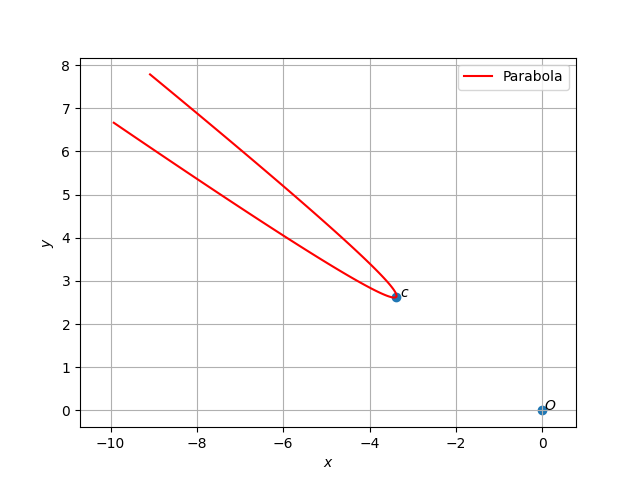
\includegraphics[width=\columnwidth]{./solutions/41/6/parab.png}
        \caption{Graph of $9x^2+24xy+16y^2-4y-x+7=0$}
        \label{eq:solutions/41/6/myfig}
\end{figure}

%
\item Trace the parabola and find its focus.
\begin{align}
144y^2-120xy+25x^2+619x-272y+663=0
\end{align}
%
%
\solution
The general second degree equation can be expressed as follows,
\begin{align}
\Vec{x}^T\Vec{V}\Vec{x}+2\Vec{u}^T\Vec{x}+f=0
\intertext{where,}
\vec{V} &= \myvec{144&-60\\-60&25}\\ \label{eq:solutions/41/7/eq:conics/ex/solution/given1}
\vec{u} &= \myvec{\cfrac{619}{2}\\-136}\\ 
f &= 663 \label{eq:solutions/41/7/eq:conics/ex/solution/given2}
\end{align}
\begin{enumerate}
\item Expanding the determinant of $\vec{V}$ we observe, 
\begin{align}
\mydet{144&-60\\-60&25} = 0 \label{eq:solutions/41/7/eq:conics/ex/solution/eq2.1}
\end{align}
Also
\begin{align}
    \mydet{\vec{V} & \vec{u} \\ \vec{u}^T & f}=
    \mydet{144&-60 & \cfrac{619}{2} \\-60&25 & -136 \\ \cfrac{619}{2} & -136 & 663} \\
    \neq 0\label{eq:solutions/41/7/eq:conics/ex/solution/eq2.2}
\end{align}
Hence from \eqref{eq:solutions/41/7/eq:conics/ex/solution/eq2.1} and \eqref{eq:solutions/41/7/eq:conics/ex/solution/eq2.2} we conclude that given equation is an parabola. The characteristic equation of $\vec{V}$ is given as follows,
\begin{align}
\mydet{\lambda\vec{I}-\vec{V}} = \mydet{\lambda-144&60\\60&\lambda-25} &= 0\\
\implies \lambda^2-169\lambda &= 0\label{eq:solutions/41/7/eq:conics/ex/solution/eqchar}
\end{align}
Hence the characteristic equation of $\vec{V}$ is given by \eqref{eq:solutions/41/7/eq:conics/ex/solution/eqchar}. The roots of \eqref{eq:solutions/41/7/eq:conics/ex/solution/eqchar} i.e the eigenvalues are given by
\begin{align}
\lambda_1=0, \lambda_2=169\label{eq:solutions/41/7/eq:conics/ex/solution/eqeigenvals}    
\end{align}
\item For $\lambda_1 = 0$, the eigen vector $\vec{p}$ is given by 
\begin{align}
\vec{V}\vec{p} = 0
\end{align}
Row reducing $\vec{V}$ yields
\begin{align}
\implies
\myvec{-144&60\\60&-25}\xleftrightarrow[R_2=R_2+5R_1]{R_1=\frac{R_1}{12}}\myvec{-12&5\\0&0}\\
\implies\vec{p}_1=\cfrac{1}{13}\myvec{5\\12} \label{eq:solutions/41/7/eq:conics/ex/solution/eq2.3}
\end{align}
Similarly, 
\begin{align}
\vec{p}_2=\frac{1}{13}\myvec{12\\-5} 
\end{align}
%
Thus, the eigenvector rotation matrix and the eigenvalue matrix are
\begin{align}
\vec{P}&=\myvec{\vec{p_1}&\vec{p_2}}=\frac{1}{13}\myvec{5&12\\ 12 &-5} \\
\vec{D}&=\myvec{0&0\\0&169}
\end{align}
The focal length of the parabola is given by 
\begin{align}
\frac{\abs{2\vec{u}^T\vec{p_1}}}{\lambda_2}
    = \frac{13}{169}=\cfrac{1}{13}
\end{align}
and its equation is
\begin{align}
    \vec{y^T}\vec{D}\vec{y}&=-\eta\myvec{1&0}\vec{y}\label{eq:solutions/41/7/eq:conics/ex/solution/eq2.4}
\end{align}
where
\begin{align}
    \eta=2\vec{u}^T\vec{p_1}=-13
\end{align}
and the vertex $\vec{c}$ is given by 
\begin{align}
    \myvec{\vec{u^T}+\frac{\eta}{2}\vec{p_1^T} \\ \vec{V}}\vec{c}=
    \myvec{-f \\\frac{\eta}{2}\vec{p_1}-\vec{u}} 
\end{align}
using equations \eqref{eq:solutions/41/7/eq:conics/ex/solution/given1},\eqref{eq:solutions/41/7/eq:conics/ex/solution/given2} and \eqref{eq:solutions/41/7/eq:conics/ex/solution/eq2.3}
\begin{align}
    \myvec{307& -142 \\ 144 & -60 \\  -60 & 25 }\vec{c}=\myvec{-663 \\ -312\\ 130} \label{eq:solutions/41/7/eq:conics/ex/solution/eqcen}
\end{align}
Forming the augmented matrix and row reducing it:
\begin{align}
\myvec{307 & -142 & -663\\144 & -60 & -312 \\-60 & 25 &130 }\\
R_2\leftrightarrow \cfrac{R_2}{12} \nonumber \\
\myvec{307 & -142 & -663\\12 & -5 & -26 \\-60 & 25 &130}\\
R_3\leftrightarrow R_3+5R_2 \nonumber \\
\myvec{307 & -142 & -663\\12 & -5 & -26 \\0 & 0 &0}\\
R_1\leftrightarrow \cfrac{R_1}{307} \nonumber \\
\myvec{1 & \cfrac{-142}{307} & \cfrac{-663}{307}\\0 & \cfrac{169}{307} & \cfrac{-26}{307} \\0 & 0 &0}\\ R_2\leftrightarrow R_2-12R_1 \nonumber \\
\myvec{1 & \cfrac{-142}{307} & \cfrac{-663}{307}\\0 & 1 & \cfrac{-26}{307} \\0 & 0 &0}\\
R_1\leftrightarrow R_1 +(142/307)R_2 \nonumber \\
\myvec{1 & 0 & -29/13\\0 & 1 & -2/13 \\0 & 0 &0}
\end{align}
Thus the vertex $\vec{c}$ is:
\begin{align}
\vec{c}=\myvec{ -29/13\\-2/13} 
\end{align}

The direction vector of axis of symmetry is given by :
\begin{align}
\vec{m}=\vec{Vc}+\vec{u}\\
=\myvec{144&-60\\-60&25}\myvec{-\cfrac{29}{13}\\-\cfrac{2}{13}}+\myvec{\cfrac{619}{2}\\-\cfrac{272}{2}}\\
=\myvec{-\cfrac{5}{2}\\-6}\\
\vec{m}=\cfrac{13}{2}\\
\implies \cfrac{\vec{m}}{\norm{\vec{m}}}=\myvec{-\cfrac{5}{13}\\-\cfrac{12}{13}}
\end{align}

The focus is given by:
\begin{align}
\vec{F}=\vec{c}-
\brak{
\frac
{
\vec{m}
}
{
\norm
{
\vec{m}
}
\times a
}
}
\\
=\myvec
{
-\cfrac{29}{13}
\\
-\cfrac{2}{13}
}
-\myvec
{
\myvec
{
-\cfrac{5}{13}
\\
-\cfrac{12}{13}
}
}
\times \cfrac{1}{52}\\
=\myvec{
-\cfrac{1503}{676}
\\
-\cfrac{23}{169}
}
\end{align}

\begin{figure}[!ht]
    \centering
    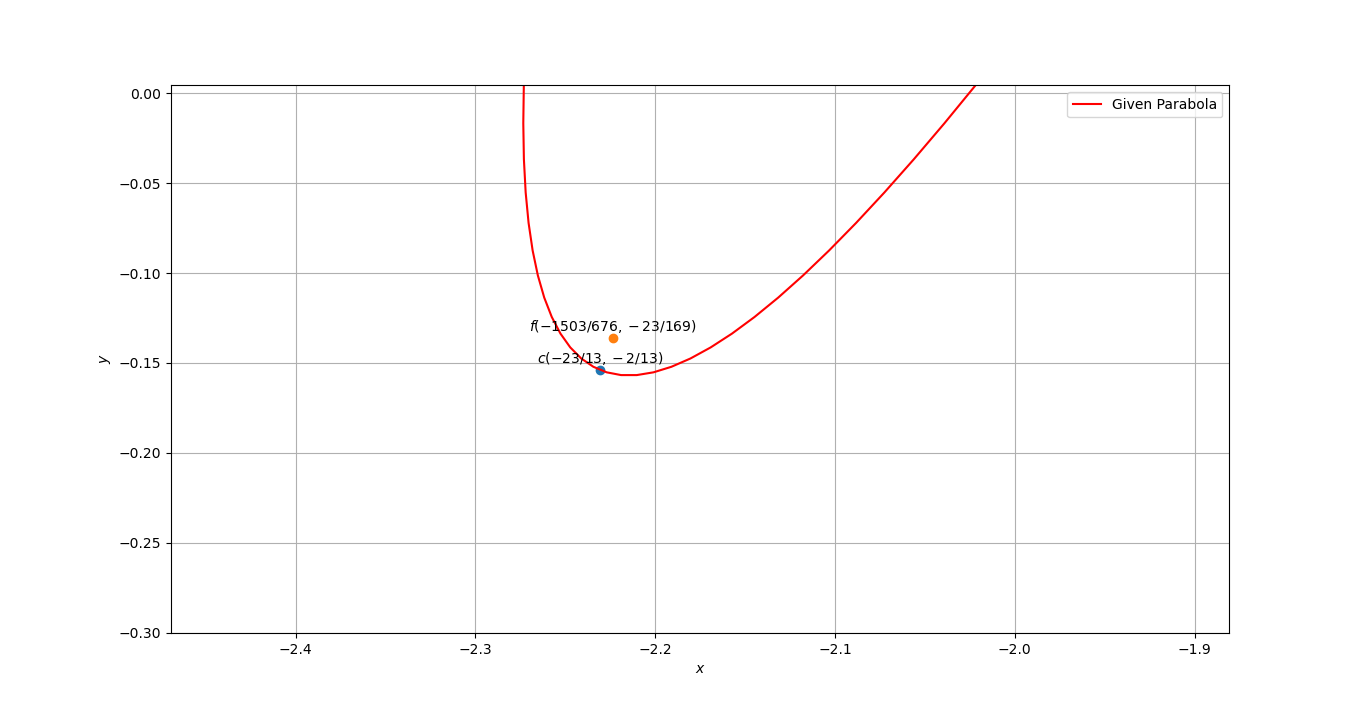
\includegraphics[width=\columnwidth]{./solutions/41/7/figs/parabola}
\caption{Traced parabola}
\label{eq:solutions/41/7/parabola}
\end{figure}

\end{enumerate}




\item Trace the parabola
\begin{align}
   16x^2-24xy+9y^2+32x+86y-39=0 \label{eq:solutions/41/8/eq:given}
\end{align}
%
\solution
The general equation of a second degree can be expressed as: 
\begin{align}
   \vec{x}^T\vec{V}\vec{x}+2\vec{u}^T\vec{x}+f=0 \label{eq:solutions/41/8/eq:conic}
\end{align}
Comparing \eqref{eq:solutions/41/8/eq:given} and \eqref{eq:solutions/41/8/eq:conic}
\begin{align}
\vec{V}=\vec{V}^T =\myvec{16 & -12 \\ -12 & 9 }, \quad\vec{u}=\myvec{16 \\ 43},\quad f=-39 \label{eq:solutions/41/8/eq:parametrics}
\end{align}
{Eigen Values:}
The characteristic equation of $\vec{V}$ is given as
\begin{align}
\mydet{\lambda \vec{I}-\vec{V}} = 0
\end{align}
\begin{align}
\implies \mydet{\lambda-16 & 12 \\ 12 & \lambda-9} =0
\end{align}
\begin{align}
\implies \lambda^2-25\lambda=0 \label{eq:solutions/41/8/eq:chartistic}
\end{align}
The eigenvalues are the roots of the equation \eqref{eq:solutions/41/8/eq:chartistic}, which are as follows:
\begin{align}
 \lambda_1=0, \quad  \lambda_2=25 \label{eq:solutions/41/8/eq:eigenval}
\end{align}
{Eigen Vectors:}
The eigen vector $\vec{p}$ is defined as
\begin{align}
\vec{V}\vec{p}=\lambda\vec{p}     
\end{align}
\begin{align}
\implies (\lambda \vec{I} - \vec{V} ) \vec{p} = 0
\end{align}
For $\lambda_1 = 0 $
\begin{align}
(\lambda_1 \vec{I}-\vec{V} ) = \myvec{-16 & 12 \\ 12 & -9 }\xleftrightarrow[R_2\leftarrow R_2+3R_1]{R_1\leftarrow \frac{1}{4}R_1}\myvec{-4 & 3\\0 & 0}
\end{align}
\begin{align}
\implies \vec{p_1} = \frac{1}{5} \myvec{3 \\ 4} \label{eq:solutions/41/8/eq:p1val}
\end{align}
For $\lambda_2 = 25$
\begin{align}
(\lambda_2 \vec{I}-\vec{V} ) = \myvec{9 & 12 \\ 12 & 1}\xleftrightarrow[R_2\leftarrow R_2-4R_1]{R_1\leftarrow \frac{1}{3}R_1}\myvec{3 & 4\\0 & 0}
\end{align}
\begin{align}
\implies \vec{p_2} = \frac{1}{5} \myvec{-4\\ 3} \label{eq:solutions/41/8/eq:p2val}
\end{align}
{Eigen Value Decomposition:}
Using EVD, we can write 
\begin{align}
 \vec{D} = \vec{P} \vec{V} \vec{P}^T
\end{align}
From \eqref{eq:solutions/41/8/eq:p1val} and \eqref{eq:solutions/41/8/eq:p2val}
\begin{align}
 \vec{P} = \frac{1}{5} \myvec{3 & -4 \\ 4 & 3}
\end{align}
From \eqref{eq:solutions/41/8/eq:eigenval}
\begin{align}
 \vec{D} = \myvec{\lambda_1 & 0 \\ 0 & \lambda_2} = \myvec{0 & 0 \\ 0 & 25}
\end{align}
{Parabola}
\begin{align}
\text{Focal Length} = \abs{\frac{2\eta}{\lambda_2}} \label{eq:solutions/41/8/eq:focallen}\\
\intertext{From \eqref{eq:solutions/41/8/eq:p1val} and \eqref{eq:solutions/41/8/eq:parametrics}}
\eta = \vec{p}_1^T\vec{u} = 44 \label{eq:solutions/41/8/eq:etaval}\\
\intertext{Substituting values of \eqref{eq:solutions/41/8/eq:etaval} and \eqref{eq:solutions/41/8/eq:eigenval} in \eqref{eq:solutions/41/8/eq:focallen}, we get}
\text{Focal Length} = \abs{\frac{88}{25}}=3.52
\end{align}
The standard equation of parabola is given by:
\begin{align}
 \vec{y}^T\vec{D}\vec{y} = -2\eta \myvec{1 & 0}\vec{y} \label{eq:solutions/41/8/eq:parabola}
\end{align}
And the vertex $\vec{c}$ is:
\begin{align}
 \myvec{\vec{u}^T+\eta \vec{p_1}^T \\ \vec{V}}\vec{c} = \myvec{-f \\ \eta \vec{p_1}-\vec{u}}
\end{align}
From \eqref{eq:solutions/41/8/eq:parametrics} \eqref{eq:solutions/41/8/eq:etaval} and \eqref{eq:solutions/41/8/eq:p1val},
\begin{align}
\myvec{\frac{212}{5} & \frac{391}{5} \\ 16 & -12 \\ -12 & 9}\vec{c}=\myvec{39 \\ \frac{52}{5}\\ \frac{-39}{5}}
\end{align}
To find $\vec{c}$, perform row reduction on the augmented matrix as follows:
\begin{align}
    \myvec{\frac{212}{5} & \frac{391}{5} & 39\\16 & -12 & \frac{52}{5}\\-12 & 9 & \frac{-39}{5}}\xleftrightarrow[R_1\leftarrow \frac{5}{212}R_1]{R_3\leftarrow R_3+\frac{3}{4}R_2}\myvec{1 & \frac{391}{212} & \frac{195}{212}\\16 & -12 & \frac{52}{5}\\0&0&0}\\
    \xleftrightarrow{R_2\leftarrow R_2-16R_1}\myvec{ 1 & \frac{391}{212} & \frac{195}{212}\\0 & \frac{-2200}{53} & \frac{-1144}{265} \\0&0&0}\\\xleftrightarrow{R_2\leftarrow \frac{-53}{2200}R_2}\myvec{1 & \frac{391}{212} & \frac{195}{212} \\0 & 1 & \frac{13}{125}\\0&0&0}\\\xleftrightarrow{R_1\leftarrow R_1-\frac{391}{212}R_2}\myvec{1 & 0 & \frac{4823}{6625}\\0 & 1 & \frac{13}{125}\\0&0&0}
\end{align}
Hence,
\begin{align}
\vec{c}=\myvec{\frac{4823}{6625}\\ \frac{13}{125}}= \myvec{0.728 \\ 0.104}
\end{align}
\begin{figure}[h!]
	\centering
	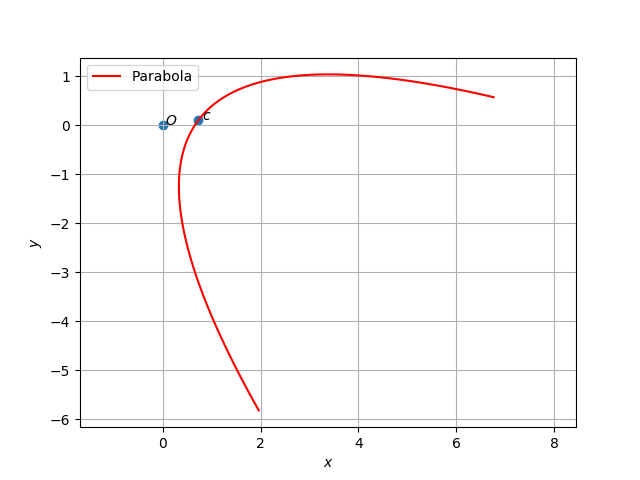
\includegraphics[width=\columnwidth]{./solutions/41/8/Codes/A5.png}
	\caption{Parabola with vertex c }
	\label{eq:solutions/41/8/myfig}
\end{figure}

\item Trace the following parabola
\begin{align}
    4x^2-4xy+y^2-12x+6y+9=0
\end{align}
%
%
\solution
The given quadratic equation can be written in the matrix form as
\begin{align}
    \vec{x}^T\myvec{4&-2\\-2&1}\vec{x}+2\myvec{-6&3}\vec{x}+9=0\label{eq:solutions/41/9/eq:1}
\end{align}
Calculating the parameters,we get
\begin{align}
    \mydet{\vec{V}}=\mydet{4&-2\\-2&1}=0\\
    \mydet{\vec{V}&\vec{u}\\\vec{u}^T&f}=\mydet{4&-2&-6\\-2&1&3\\-6&3&9}=0
\end{align}
Therefore the given parabola equation is a degenerate.The quadratic equation corresponds to a pair of coincident straight lines.\par
The characteristic equation of $\vec{V}$ will be
\begin{align}
    \mydet{\vec{V}-\lambda\vec{I}}&=\mydet{4-\lambda&-2\\-2&1-\lambda}\\
    &=\lambda^2-5\lambda\\
    &\lambda_1=0,\lambda_2=5
\end{align}
The eigen vectors are the nullspace of the matrix $\vec{V}-\lambda\vec{I}$.For $\lambda_1=0$
\begin{align}
    \myvec{4&-2\\-2&1}\xleftrightarrow{R_2=2R_2+R_1}\myvec{4&-2\\0&0}\\
    p_1=\myvec{1\\2}
\end{align}
Therefore the normalized eigen vector will be
\begin{align}
    p_1=\myvec{\frac{1}{\sqrt{5}}\\\frac{2}{\sqrt{5}}}
\end{align}
For $\lambda_2=5$
\begin{align}
    \myvec{-1&-2\\-2&-4}\xleftrightarrow{R_2=R_2-2R_1}\myvec{-1&-2\\0&0}\\
    p_2=\myvec{-2\\1}
\end{align}
Therefore the normalized eigen vector will be
\begin{align}
    p_2=\myvec{-\frac{2}{\sqrt{5}}\\\frac{1}{\sqrt{5}}}
\end{align}
Therefore the transformation matrix will be
\begin{align}
    \vec{P}=\myvec{p_1&p_2}=\myvec{\frac{1}{\sqrt{5}}&-\frac{2}{\sqrt{5}}\\\frac{2}{\sqrt{5}}&\frac{1}{\sqrt{5}}}
\end{align}
The value of $\eta$ will be
\begin{align}
    \eta&=2p_1^T\vec{u}\\
    &=2\myvec{\frac{1}{\sqrt{5}}&\frac{2}{\sqrt{5}}}\myvec{-6\\3}\\
    &=0
\end{align}
A point on the line can be found by using to following formula
\begin{align}
    \myvec{\vec{u}^T+\frac{\eta}{2}p_1^T\\\vec{V}}c=\myvec{-f\\\frac{\eta}{2}p_1-\vec{u}}\\
    \myvec{\vec{u}^T\\\vec{V}}c=\myvec{-f\\-\vec{u}}\\
    \myvec{-6&3\\4&-2\\-2&1}c=\myvec{-9\\6\\-3}
\end{align}
Writing it in augmented form, we get
\begin{align}
    \myvec{-6&3&-9\\4&-2&6\\-2&1&-3}\xleftrightarrow{R_3=R_3-\frac{R_1}{3}}\myvec{-6&3&-9\\4&-2&6\\0&0&0}\\
    \xleftrightarrow{R_2=\frac{3}{2}R_2+R_1}\myvec{-6&3&-9\\0&0&0\\0&0&0}
\end{align}
Therefore we can see that the point $c=\myvec{1\\-1}$ lies on the line.
{Equation of the straight line}
Applying affine transformation we get
\begin{align}
    \vec{y}^T\vec{D}\vec{y}=-\eta\myvec{1&0}\vec{y}\\
    \vec{y}^T\myvec{0&0\\0&5}\vec{y}=0\\
    5y^2=0
\end{align}
Therefore the transformed line is $y=0$,which in vector form will be $\myvec{0&1}\vec{y}=0$.\par
Taking the Inverse affine transformation we get
\begin{align}
    \myvec{0&1}\brak{P^T\brak{\vec{x}-c}}=0\\
    \myvec{0&1}\myvec{\frac{1}{\sqrt{5}}&\frac{2}{\sqrt{5}}\\-\frac{2}{\sqrt{5}}&\frac{1}{\sqrt{5}}}\brak{\vec{x}-c}=0\\
    \myvec{-\frac{2}{\sqrt{5}}&\frac{1}{\sqrt{5}}}\brak{\vec{x}-c}=0\\
    \myvec{-\frac{2}{\sqrt{5}}&\frac{1}{\sqrt{5}}}\vec{x}-\myvec{-\frac{2}{\sqrt{5}}&\frac{1}{\sqrt{5}}}\myvec{1\\-1}=0\\
    \myvec{-\frac{2}{\sqrt{5}}&\frac{1}{\sqrt{5}}}\vec{x}+\frac{3}{\sqrt{5}}=0\\
    \myvec{2&-1}\vec{x}=3
\end{align}
Therefore the equation of coincident lines is $\brak{2x-y-3}=0$.

%
\item Trace the central conic,
\begin{align}
2x^2 - 2xy + y^2 + 2x - 2y = 0\label{eq:solutions/41/17/eq:1}
\end{align}
%
\\
\solution
The general equation of a second degree (In algebraic form) can be expressed as,
\begin{align}
ax^2 + 2bxy + cy^2 + 2dx + 2ey + f = 0 \label{eq:solutions/41/17/eq:2}
\end{align}
The general equation of a second degree (In vector form) can be expressed as,
\begin{align}
\vec{x^T}\vec{V}\vec{x} + 2\vec{u^T}\vec{x} + f = 0
\end{align}
Comparing \eqref{eq:solutions/41/17/eq:1} with \eqref{eq:solutions/41/17/eq:2} , we get,
\begin{align}
a = 2, \ b = -1, \ c = 1, \ d = 1, \ e = -1 \ and \ f = 0
\end{align}
where,
\begin{align}
\vec{V} = \myvec{a & b \\ b & c} = \myvec{2 & -1 \\ -1 & 1} = \vec{V^T}\\
\implies \vec{V} = \myvec{2 & -1 \\ -1 & 1}
\end{align}
and
\begin{align}
\vec{u} = \myvec{1 \\ -1}    
\end{align}
Finding the determinant of V we obtain, 
\begin{align}
|\vec{V}| = 1 > 0
\end{align}
which means the given central conic is an ellipse which can be proven more effectively using,
\begin{align}
\vec{V} = \vec{PDP^T}\label{eq:solutions/41/17/eq:9}    
\end{align}
where $\vec{P}$ is a matrix of Eigen vectors and $\vec{D}$ is a diagonal matrix of Eigen values which will be computed subsequently.\\
Computing Eigen values for $\vec{V}$ using the characteristic equation of the matrix, we get the following quadratic equation in terms of $\lambda$
\begin{align}
\lambda^{2} - 3\lambda + 1 = 0\\
\implies \lambda_{1} = \frac{3 + \sqrt{5}}{2} \ and \ \lambda_{2} = \frac{3 - \sqrt{5}}{2}
\end{align}
Eigen vectors can be computed using the following equation,
\begin{align}
(\lambda\vec{I - V})\vec{p} = 0
\end{align}
Solving this for $\lambda_{1}$ and $\lambda_{2}$ respectively and normalizing them we obtain,
\begin{align}
\vec{p_1} = \sqrt{\frac{2}{5-\sqrt{5}}}\myvec{1 \\[1em] \frac{1-\sqrt{5}}{2}}\\
\vec{p_2} = \sqrt{\frac{2}{5+\sqrt{5}}}\myvec{1 \\[1em] \frac{\sqrt{5}+1}{2}}
\end{align}
Simplifying, 
\begin{align}
\implies \vec{P} = \myvec{\sqrt{\frac{2}{5-\sqrt{5}}} & \sqrt{\frac{2}{5+\sqrt{5}}} \\[1em] \frac{1-\sqrt{5}}{\sqrt{5\sqrt{2}-\sqrt{10}}} & \frac{1+\sqrt{5}}{\sqrt{5\sqrt{2}+\sqrt{10}}}} \label{eq:solutions/41/17/eq:15}
\end{align}
\begin{align}
\vec{D} = \myvec{\frac{3+\sqrt{5}}{2} & 0 \\ 0 & \frac{3-\sqrt{5}}{2}}
\end{align}
Using \eqref{eq:solutions/41/17/eq:9} can verify that it holds which means that the given central conic is an ellipse.
The center of the ellipse can be computed using,
\begin{align}
\vec{c} = \vec{-V^{-1}u}\\
\implies \vec{c} = \myvec{0 \\ 1} \label{eq:solutions/41/17/eq:18}
\end{align}
The parameters of the ellipse are computed as follows,
\begin{align}
\sqrt{\frac{{\vec{u^{T}V^{-1}u} - f}}{\lambda_{1}}} = \sqrt{\frac{3-\sqrt{5}}{2}}\\
\sqrt{\frac{{\vec{u^{T}V^{-1}u} - f}}{\lambda_{2}}} = \sqrt{\frac{3+\sqrt{5}}{2}}
\end{align}
The angle of Rotation can be obtained by equating $\vec{P}$ with the Rotation matrix which is,
\begin{align}
\vec{P} = \myvec{\cos{\theta} & \sin{\theta} \\ -\sin{\theta} & cos{\theta}} \label{eq:solutions/41/17/eq:21}
\end{align}
Comparing \eqref{eq:solutions/41/17/eq:15} and \eqref{eq:solutions/41/17/eq:21} we get,
\begin{align}
\theta = \frac{\pi}{5.66} \label{eq:solutions/41/17/eq:22}  
\end{align}
Using the Affine transformation we find out the actual ellipse,
\begin{align}
\vec{y} = \vec{P^Tx} + \vec{c}     
\end{align}
which means the actual ellipse is obtained by translating and rotating the standard ellipse w.r.t center, $\vec{c}$ from \eqref{eq:solutions/41/17/eq:18} and angle of rotation, $\theta$ from \eqref{eq:solutions/41/17/eq:22} respectively.\\
Using the above data along with $\vec{o}$ (Origin), the center of the standard ellipse, the actual ellipse is plotted as follows.  
\begin{figure}[!ht]
    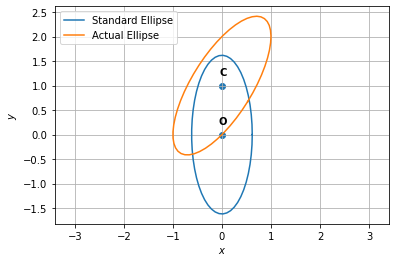
\includegraphics[width=\columnwidth]{solutions/41/17/Figure.png}
    \caption{Standard and Actual Ellipses}
    \label{eq:solutions/41/17/Fig.1}
\end{figure}

\item Trace the following central conic : 
\begin{align}
    x^2+y^2+xy+x+y=1\label{eq:solutions/41/18/eq:0}
\end{align}
%
\\
\solution
General equation of second degree is given by :
\begin{align}
\vec{x}^T\vec{V}\vec{x}+2\vec{u}^T\vec{x}+f=0\label{eq:solutions/41/18/eq:1}
\end{align}
In the vector form \eqref{eq:solutions/41/18/eq:0} can be written as :
\begin{align}
\vec{x}^T\myvec{1&\frac{1}{2}\\[0.1cm]\frac{1}{2}&1}\vec{x}+2\myvec{\frac{1}{2}\\[0.1 cm]\frac{1}{2}}^T\vec{x}-1=0\label{eq:solutions/41/18/eq:2}
\end{align}
By comparing \eqref{eq:solutions/41/18/eq:1} and \eqref{eq:solutions/41/18/eq:2} we get : 
\begin{align}
    \vec{V}=\myvec{1&\frac{1}{2}\\[0.1cm]\frac{1}{2}&1},\vec{u}=\myvec{\frac{1}{2}\\[0.1 cm]\frac{1}{2}},f=-1\label{eq:solutions/41/18/eq:3}
\end{align}
Eigen values for matrix $\vec{V}$ can be calculated by solving :  
\begin{align}
    \mydet{1-\lambda&\frac{1}{2}\\[0.1cm]\frac{1}{2}&1-\lambda}&=0\\
    \lambda^2-2\lambda+\frac{3}{4}&=0\\
    \lambda_1=\frac{3}{2},\lambda_2&=\frac{1}{2}
\end{align}
By doing Eigenvalue Decomposition and Affine Transformation we get : 
\begin{align}
    \vec{P}^{-1}\vec{V}\vec{P}&=\vec{D}=\myvec{\lambda_1&0\\0&\lambda_2}\\
    \vec{x}&=\vec{P}\vec{y}+\vec{c}\label{eq:solutions/41/18/eq:8}
\end{align}
Where the matrix $\vec{P}$ is normalised eigenbasis and $\vec{c}$ is the center.\\
By putting the value of $\vec{x}$ from \eqref{eq:solutions/41/18/eq:8} in \eqref{eq:solutions/41/18/eq:1} we get : 
\begin{align}
    (\vec{P}\vec{y}+\vec{c})^T\vec{V}(\vec{P}\vec{y}+\vec{c})+2\vec{u}^T\vec{x}+f=0
\end{align}
Further solving this we get : 
\begin{align}
    \vec{V}\vec{c}+\vec{u}&=0\implies\vec{c}=-\vec{V}^{-1}\vec{u}\label{eq:solutions/41/18/eq:10}\\
    \vec{y}^T\vec{D}\vec{y}&=\vec{u}^T\vec{V}^{-1}\vec{u}-f\label{eq:solutions/41/18/eq:11}
\end{align}
As
\begin{align}
    \mydet{\vec{V}} =\mydet{1&\frac{1}{2}\\[0.1cm]\frac{1}{2}&1}=\frac{3}{4}>0
\end{align}
Equation \eqref{eq:solutions/41/18/eq:11} forms an ellipse centered at origin with major and minor axis given as : 
\begin{align}
    a=\sqrt{\frac{\vec{u}^T\vec{V}^{-1}\vec{u}-f}{\lambda_1}}\label{eq:solutions/41/18/eq:13}\\
    b=\sqrt{\frac{\vec{u}^T\vec{V}^{-1}\vec{u}-f}{\lambda_2}}\label{eq:solutions/41/18/eq:14}
\end{align} 
Using Gauss Jordan Elimination on matrix $\vec{V}$ : 
\begin{align}
 \xleftrightarrow{R_2 \leftarrow \frac{1}{2} R_1-R_2}\myvec{1&\frac{1}{2}&:&1&0\\[0.1cm]0&\frac{-3}{4}&:&\frac{1}{2}&-1}\\
 \xleftrightarrow{R_2 \leftarrow \frac{-4}{3} R_2}\myvec{1&\frac{1}{2}&:&1&0\\[0.1cm]0&1&:&\frac{-2}{3}&\frac{4}{3}}\\
 \xleftrightarrow{R_1 \leftarrow R_1-\frac{1}{2} R_2}\myvec{1&0&:&\frac{4}{3}&\frac{-2}{3}\\[0.1cm]0&1&:&\frac{-2}{3}&\frac{4}{3}}
 \end{align}
 Therefore,
 \begin{align}
 \vec{V}^{-1}=\myvec{\frac{4}{3}&\frac{-2}{3}\\[0.2cm]\frac{4}{3}&\frac{-2}{3}}\label{eq:solutions/41/18/eq:18}
\end{align}
Using \eqref{eq:solutions/41/18/eq:10} and \eqref{eq:solutions/41/18/eq:18} we get : 
\begin{align}
    \vec{c}=-\vec{V}^{-1}\vec{u}=-\myvec{\frac{4}{3}&\frac{-2}{3}\\[0.2cm]\frac{4}{3}&\frac{-2}{3}}\myvec{\frac{1}{2}\\[0.2cm]\frac{1}{2}}=\myvec{\frac{-3}{10}\\[0.2cm]\frac{-3}{10}}
\end{align}
By putting the values of $\vec{u}$, $\vec{V}^{-1}$, $f$, $\lambda_1$ and $\lambda_2$ in \eqref{eq:solutions/41/18/eq:13} and \eqref{eq:solutions/41/18/eq:14} respectively we get :   
\begin{align}
    a&=\sqrt{\frac{\myvec{\frac{1}{2}&\frac{1}{2}}\myvec{\frac{4}{3}&\frac{-2}{3}\\[0.2cm]\frac{4}{3}&\frac{-2}{3}}\myvec{\frac{1}{2}\\[0.2cm]\frac{1}{2}}-1}{\frac{3}{2}}}=\frac{9}{10}\\
    b&=\sqrt{\frac{\myvec{\frac{1}{2}&\frac{1}{2}}\myvec{\frac{4}{3}&\frac{-2}{3}\\[0.2cm]\frac{4}{3}&\frac{-2}{3}}\myvec{\frac{1}{2}\\[0.2cm]\frac{1}{2}}-1}{\frac{1}{2}}}=\frac{8}{5}
\end{align}

In the transformed space with Eigenbasis, an ellipse centered at origin with major and minor axis as $a$ and $b$ is traced as 'Standard Ellipse' in the plot.\\


And after doing Affine Transformation on $\vec{y}$ as in \eqref{eq:solutions/41/18/eq:8} we get our 'Actual Ellipse' centered at $\vec{c}$ shown in the plot.
\begin{figure}[h]
\centering
    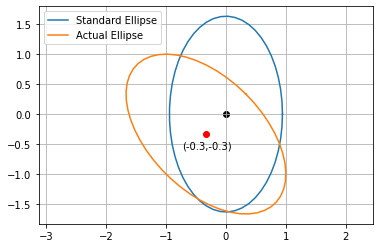
\includegraphics[width=\columnwidth]{solutions/41/18/ellipse.png}
    \caption{Standard Ellipse centered at origin and Actual Ellipse centered at $(-0.3,-0.3)$.}
    \label{eq:solutions/41/18/tangent}
\end{figure}

\item Trace the following central conic:
\begin{align}
  2x^2 + 3xy - 2y^2 - 7x + y - 2 = 0 \label{eq:solutions/41/19/eq:1}
\end{align}
%
\\
\solution
Any second degree equation of the form:
\begin{align}
  ax^2 + 2bxy + cy^2 + 2dx + 2ey + f = 0
\end{align}
Can be represented in matrix / vector form as:
\begin{align}
  \vec{x}^T\vec{Vx} + 2\vec{u}^T\vec{x} + f = 0
\end{align}
where,
\begin{align}
  \vec{V} = \vec{V}^T = \myvec{a & b \\ b & c} \\
  \vec{u} = \myvec{d & e}
\end{align}
Rewriting \eqref{eq:solutions/41/19/eq:1} in matrix form, we get:
\begin{align}
  \vec{x}^T\myvec{2 & \frac{3}{2} \\\frac{3}{2} & -2}\vec{x} + 2\myvec{-\frac{7}{2} & \frac{1}{2}} - 2 = 0
\end{align}
where,
\begin{align}
  \vec{V} = \myvec{2 & \frac{3}{2} \\\frac{3}{2} & -2} \\
  \vec{u} = \myvec{-\frac{7}{2} \\[0.2cm] \frac{1}{2}} \\
  f = -2 \\
  det(\vec{V}) = \mydet{2 & \frac{3}{2} \\\frac{3}{2} & -2} = -\frac{25}{4}
\end{align}
As $det(\vec{V}) < 0$, the given conic represents a hyperbola. \\
The characteristic equation of $\vec{V}$ is given by the determinant:
\begin{align}
  \mydet{\vec{V} - \lambda\vec{I}} = 0 \\
  \mydet{2 - \lambda & \frac{3}{2} \\\frac{3}{2} & -2 - \lambda} = 0 \\
  \implies \lambda^{2} - \frac{25}{4} = 0 \label{eq:solutions/41/19/eq:2}
\end{align}
The roots of \eqref{eq:solutions/41/19/eq:2} (the eigenvalues) are:
\begin{align}
  \lambda_1 = \frac{5}{2}, \lambda_2 = -\frac{5}{2}
\end{align}
The eigenvector $\vec{p}$ is defined as:
\begin{align}
  \vec{Vp} = \lambda \vec{p} \\
  \implies (\vec{V} - \lambda \vec{I})\vec{p} = 0 \label{eq:solutions/41/19/eq:3}
\end{align}
Evaluating \eqref{eq:solutions/41/19/eq:3} for $\lambda_1 = \frac{5}{2}$, we get:
\begin{align}
  (\vec{V} - \lambda_1 \vec{I})  = \myvec{-\frac{1}{2} & \frac{3}{2} \\[0.2cm]\frac{3}{2} & -\frac{9}{2}}
\end{align}
Reducing the above equation to row-echelon form, we get:
\begin{align}
  \xleftrightarrow[]{R_2 \rightarrow R_2 + 3R_1} \myvec{-\frac{1}{2} & \frac{3}{2} \\[0.2cm]0 & 0} \xleftrightarrow[]{R_1 \rightarrow -2R_1} \myvec{1 & -3 \\ 0 & 0} \label{eq:solutions/41/19/eq:4}
\end{align}
Substituting \eqref{eq:solutions/41/19/eq:4} in \eqref{eq:solutions/41/19/eq:3}, we get:
\begin{align}
  \myvec{1 & -3 \\ 0 & 0} \myvec{v_1 \\ v_2} = \myvec{0 \\ 0}
\end{align}
where,
\begin{align}
  \vec{p} = \myvec{v_1 \\ v_2}
\end{align}
Let $v_2 = t$. Then
\begin{align}
  v_1 = 3t
\end{align}
Let $t = 1$. The eigenvector $\vec{p_1}$ is:
\begin{align}
  \vec{p_1} = \myvec{3 \\ 1}
\end{align}
Similarly for $\lambda_2 = -\frac{5}{2}$, we get:
\begin{align}
    (\vec{V} - \lambda_2 \vec{I})  = \myvec{\frac{9}{2} & \frac{3}{2} \\[0.2cm]\frac{3}{2} & \frac{1}{2}} \xleftrightarrow[R_1 \rightarrow \frac{2}{9}R_1]{R_2 \rightarrow 3R_2 - R_1} \myvec{1 & \frac{1}{3} \\[0.2cm]0 & 0} \label{eq:solutions/41/19/eq:5}
\end{align}
Substituting \eqref{eq:solutions/41/19/eq:5} in \eqref{eq:solutions/41/19/eq:3}, we get:
\begin{align}
  \myvec{1 & \frac{1}{3} \\[0.2cm]0 & 0} \myvec{v_1 \\ v_2} = \myvec{0 \\ 0}
\end{align}
where,
\begin{align}
  \vec{p} = \myvec{v_1 \\ v_2}
\end{align}
Let $v_2 = t$. Then
\begin{align}
  v_1 = \frac{-t}{3}
\end{align}
Let $t = 1$. The eigenvector $\vec{p_2}$ is:
\begin{align}
  \vec{p_2} = \myvec{\frac{-1}{3} \\[0.2cm] 1}
\end{align}
As $\vec{V} = \vec{V}^T$, there exists an orthogonal matrix P such that:
\begin{align}
  \vec{PVP}^T = \vec{D} = diag(\lambda_1, \lambda_2)
\end{align}
$\vec{V}$ can be rewritten using the above equation as:
\begin{align}
  \vec{V} = \vec{PDP}^T
\end{align}
where,
\begin{align}
  \vec{P} = \myvec{\vec{p_1} & \vec{p_2}} \\
  \vec{D} = \myvec{\lambda_1 & 0 \\ 0 & \lambda_2}
\end{align}
Substituting the values -
\begin{align}
  \vec{P} = \myvec{3 & \frac{-1}{3}\\[0.2cm] 1 & 1} \\
  \vec{D} = \myvec{\frac{5}{2} & 0 \\[0.2cm] 0 & \frac{-5}{2}}
\end{align}
The center of hyperbola is given by:
\begin{align}
  \vec{c} = -\vec{V}^{-1}\vec{u} \\
  \implies \vec{c} = -\myvec{\frac{8}{25} & \frac{6}{25} \\[0.2cm] \frac{6}{25} & \frac{-8}{25}} \myvec{\frac{-7}{2} \\[0.2cm]\frac{1}{2}} = \myvec{1 \\ 1}
\end{align}
As
\begin{align}
  \vec{u}^T\vec{V}^{-1}\vec{u} - f = 5 > 0
\end{align}
there is no requirement for swapping the axes (which will be evident from the equation below). The axes of the hyperbola are given by:
\begin{align}
  axes = \begin{cases}
    \sqrt[]{\frac{\vec{u}^T\vec{V}^{-1}\vec{u} - f}{\lambda_1}} \\
    \sqrt[]{\frac{f - \vec{u}^T\vec{V}^{-1}\vec{u}}{\lambda_2}}
  \end{cases} \\
  \implies \sqrt[]{\frac{\vec{u}^T\vec{V}^{-1}\vec{u} - f}{\lambda_1}} = \sqrt[]{2} \\
  \implies \sqrt[]{\frac{f - \vec{u}^T\vec{V}^{-1}\vec{u}}{\lambda_2}} = \sqrt[]{2}
\end{align}
The standard form of conic is written as:
\begin{align}
  \vec{y}^T\vec{Dy} = \vec{u}^T\vec{V}^{-1}\vec{u} - f
\end{align}
where,
\begin{align}
  \vec{y} = \vec{P}^T(\vec{x-c}) \\
  \implies \vec{y}^T \myvec{\frac{5}{2} & 0 \\[0.2cm] 0 & \frac{-5}{2}} \vec{y} -5 = 0
\end{align}
The plot of both the conics are given below:
\begin{figure}[h!]
\centering
    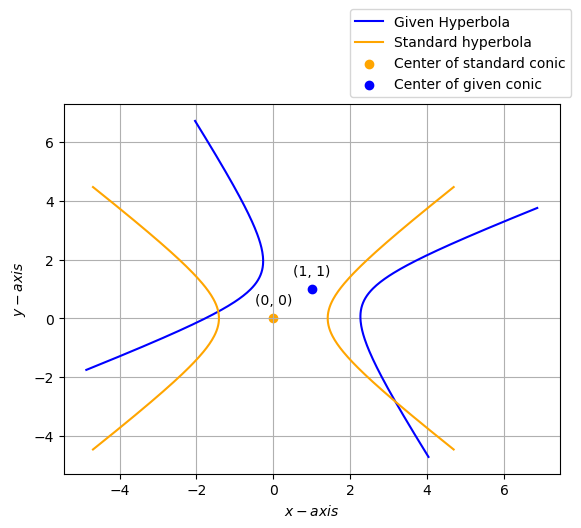
\includegraphics[width=\columnwidth]{solutions/41/19/Latex/hyperbola.png}
    \caption{Plot of given hyperbola and the standard hyperbola}
    \label{eq:solutions/41/19/fig:1}
\end{figure}

\item Trace the following central conics:
\begin{align}
   40{x^2}+36{xy}+25{y^2}-196{x}-122{y}+205=0
\end{align}
%
\\
\solution
The general equation of a second degree can
be expressed as:
\begin{align}
a{x^2}+2b{xy}+c{y^2}+2d{x}+2e{y}+f=0\label{eq:solutions/41/20/geneqn}\\
   \Longrightarrow \vec{x^TVx}+2\vec{u^Tx}+f=0\label{eq:solutions/41/20/geneqn2}
\end{align}
where\begin{align}
\vec{V} =\myvec{a\quad b\\b\quad c},\vec{u}=\myvec{d\\e}\label{eq:solutions/41/20/paraeqn} 
\end{align}
The given equation of the curve can be expressed as:
\begin{align}
    40{x^2}+2(18){xy}+25{y^2}+2(-98){x}+2(-61){y}+205=0\label{eq:solutions/41/20/giveneqn}
\end{align}
Comparing \eqref{eq:solutions/41/20/geneqn},\eqref{eq:solutions/41/20/paraeqn} and \eqref{eq:solutions/41/20/giveneqn}:\\
\begin{align}
\vec{V} = \myvec{40\quad\sqrt{18}\\\sqrt{18}\quad 25},\vec{u}=\myvec{-98\\-61} and\quad f=205 \\
       \Longrightarrow\mydet{\vec{V}}=982\quad and \quad b^2-ac=18-40.25 =-982
\end{align}
Since $\mydet{\vec{V}}>0$\quad and \quad $b^2<ac$ , \eqref{eq:solutions/41/20/giveneqn} represent an ellipse. \\
 The characteristic equation of $\vec{V}$ is given as follows,
\begin{align}
\mydet{\lambda\vec{I}-\vec{V}} = \mydet{\lambda-40\quad\sqrt{18}\\\sqrt{18}\quad\lambda -25} &= 0\\
\implies \lambda^2-65\lambda+982 &= 0\label{eq:solutions/41/20/eqchar}
\end{align}
Hence the characteristic equation of $\vec{V}$ is given by \eqref{eq:solutions/41/20/eqchar}. The roots of \eqref{eq:solutions/41/20/eqchar} i.e the eigenvalues are given by
\begin{align}
\lambda_1=\frac{65+\sqrt{297}}{2}, \lambda_2=\frac{65-\sqrt{297}}{2}\label{eq:solutions/41/20/eqeigenvals}    
\end{align}
The eigen vector $\vec{p}$ is defined as, 
\begin{align}
\vec{V}\vec{p} &= \lambda\vec{p}\\
\implies\brak{\lambda\vec{I}-\vec{V}}\vec{p}&=0\label{eq:solutions/41/20/eqneigvenvec}
\end{align}
for $\lambda_1=\frac{65+\sqrt{297}}{2}$,
\begin{align}
\brak{\lambda_1\vec{I}-\vec{V}}=\myvec{\frac{\sqrt{297}-15}{2}&-\sqrt{18}\\-\sqrt{18}&\frac{\sqrt{297}+15}{2}}\\\xleftrightarrow{R_2=R_2+\frac{2\sqrt{18}}{\sqrt{297}-15}R_1}\myvec{\frac{\sqrt{297}-15}{2}&-\sqrt{18}\\0&0}\label{eq:solutions/41/20/norm eqn1}
\end{align}
From \eqref{eq:solutions/41/20/eqneigvenvec} and \eqref{eq:solutions/41/20/norm eqn1}
\begin{align}
\implies\vec{p_1}&=\myvec{\sqrt{18}\\\frac{\sqrt{297}-15}{2}}
\end{align}
For $\lambda_2=\frac{65-\sqrt{297}}{2}$
\begin{align}
\brak{\lambda_2\vec{I}-\vec{V}}=\myvec{\frac{-\sqrt{297}-15}{2}&-\sqrt{18}\\-\sqrt{18}&\frac{15-\sqrt{297}}{2}}\\
\xleftrightarrow[R_1=-R_1]{R_2=R_2+\frac{2\sqrt{18}}{\sqrt{297}+15}R_1}\myvec{\frac{\sqrt{297}+15}{2}&\sqrt{18}\\0&0}
%\label{eq:solutions/41/20/norm eqn1}
\\
\implies\vec{p_2}=\myvec{-\sqrt{18}\\\frac{\sqrt{297}+15}{2}}
\end{align}
 \quad using the affine transformation
\begin{align}
\vec{x}&=\vec{P}\vec{y}+c
^{\prime}\intertext{such that}
\vec{P}^T\vec{V}\vec{P}=\vec{D}\quad and\quad\vec{P}&=\myvec{\vec{p_1}&\vec{p_2}},\quad\vec{P}^T=\vec{P}^{-1}\\
\intertext{Where $\vec{D}$ is a diagonal matrix, we get}
\vec{D}&=\myvec{\frac{65+\sqrt{297}}{2}&0\\0&\frac{65-\sqrt{297}}{2}}
\end{align}
Now \eqref{eq:solutions/41/20/geneqn2} can be written as,
\begin{align}
\vec{y^T}\vec{D}\vec{y}&=\vec{u^T}\vec{V^{-1}}\vec{u}-f\quad\text{$\mydet{\vec{V}}\not=0$}\label{eq:solutions/41/20/eqnewmain}\\
\intertext{And,}
\vec{c^\prime}&= -\vec{V^{-1}}\vec{u}\qquad\text{$\mydet{\vec{V}}\not=0$}\label{eq:solutions/41/20/eqcenter}\\
\vec{y} &= \vec{P^T}\brak{\vec{x-c}}\label{eq:solutions/41/20/eqY}
\end{align}
The centre of the conic section in \eqref{eq:solutions/41/20/giveneqn} is given by $\vec{c^\prime}$ in \eqref{eq:solutions/41/20/eqcenter}. 
We compute $\vec{V^{-1}}$ as follows,
\begin{align}
\myvec{40&\sqrt{18}&1&0\\\sqrt{18}&25&0&1}&\xleftrightarrow[R_1=\frac{1}{40}R_1]{R_2=R_2-\frac{\sqrt{18}}{40}R_1}\myvec{1&\frac{\sqrt{18}}{40}&\frac{1}{40}&0\\0&\frac{982}{40}&-\frac{\sqrt{18}}{40}&1}\\
&\xleftrightarrow[R_1=R_1-\frac{\sqrt{18}}{40}R_2]{R_2=\frac{40}{982}R_2}\myvec{1&0&\frac{25}{982}&-\frac{\sqrt{18}}{982}\\0&1&-\frac{\sqrt{18}}{982}&\frac{40}{982}}
\end{align}
Hence $\vec{V^{-1}}$ is given by,
\begin{align}
\vec{V^{-1}} = \myvec{\frac{25}{982}&-\frac{\sqrt{18}}{982}\\-\frac{\sqrt{18}}{982}&\frac{40}{982}}
\end{align}
Now $\vec{u^T}\vec{V^{-1}}\vec{u}$ is given by,
\begin{align}
\vec{u^T}\vec{V^{-1}}\vec{u}&=\frac{1}{982}\myvec{-98&-61}\myvec{25&-\sqrt{18}\\-\sqrt{18}&40}\myvec{-98\\-61}\\&=344.4203\label{eq:solutions/41/20/eqRHS}\\
\intertext{And, $\vec{V^{-1}}\vec{u}$ is given by,}
\vec{V^{-1}}\vec{u} &= \frac{1}{982}\myvec{25&-\sqrt{18}\\-\sqrt{18}&40}\myvec{-98\\-61}\label{eq:solutions/41/20/eqcenterRHS}\\
\end{align}
By putting the value of \eqref{eq:solutions/41/20/eqcenterRHS}, the center of the ellipse is given by \eqref{eq:solutions/41/20/eqcenter} as follows,
\begin{align}
\vec{c^\prime} = \myvec{2.231\\2.061}
\end{align}
Also the semi-major axis ($a$) and semi-minor axis ($b$) of the ellipse are given by,
\begin{align}
a = \sqrt{\frac{\vec{u^T}\vec{V^{-1}}\vec{u}-f}{\lambda_1}}=1.8414\\
b = \sqrt{\frac{\vec{u^T}\vec{V^{-1}}\vec{u}-f}{\lambda_2}}=2.416
\end{align}
Finally from \eqref{eq:solutions/41/20/eqnewmain}, the equation of ellipse is given by,
\begin{align}
&\vec{y^T}\myvec{41.116&0\\0&23.883}\vec{y}=139.4203\label{eq:solutions/41/20/eqFinal}
\end{align}
\begin{figure}[!]
 \begin{center}
  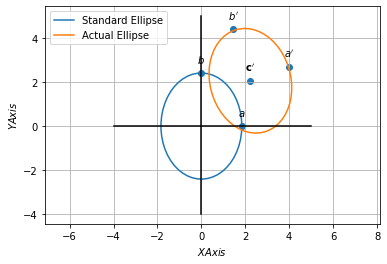
\includegraphics[width=\columnwidth]{solutions/41/20/assignment6_fig.png}
    \caption{Graphical representation of the actual curve  $40{x^2}+36{xy}+25{y^2}-196{x}-122{y}+205=0$, which represent an ellipse.}
\label{eq:solutions/41/20/myfig:1}
    \end{center}
\end{figure}

\item Trace the curve
\begin{align}
35x^2+30y^2+32x-108y-12xy+59=0 \label{eq:solutions/41/ex/given_curve_eq}
\end{align}
%
\solution
The general equation of second degree is given by
\begin{align}
ax^2+2bxy+cy^2+2dx+2ey+f=0 \label{eq:solutions/41/ex/gen_quad_eqn}
\end{align}
and can be expressed as
\begin{align}
\vec{x}^T\vec{V}\vec{x}+2\vec{u}^T\vec{x}+f=0 \label{eq:solutions/41/ex/conic_quad_eqn}
\end{align}
where
\begin{align}
\vec{V} &= \vec{V}^T = \myvec{a & b \\ b & c}
\\
\vec{u}^T &= \myvec{d & e}
\end{align}

Comparing \eqref{eq:solutions/41/ex/given_curve_eq} with \eqref{eq:solutions/41/ex/gen_quad_eqn}, we get
\begin{align}
\vec{V} &= \myvec{35  & -6 \\ -6 & 30}
\\
\vec{u}^T &= \myvec{16 & -54}
\end{align}
If $\abs{\vec{V}} > 0$, then \eqref{eq:solutions/41/ex/conic_quad_eqn} is an ellipse. 
\begin{align}
\abs{V} = 
\mydet{
35  & -6 \\ -6 & 30
}
= 1014 > 0
\end{align}
%
\eqref{eq:solutions/41/ex/conic_quad_eqn} can be expressed as
\begin{align}
\label{eq:solutions/41/ex/conic_simp_temp_nonparab_eq}
\vec{y}^T\vec{D}\vec{y} &=  \vec{u}^T\vec{V}^{-1}\vec{u} -f  &  \abs{V} &\ne 0
\\
\vec{y}^T\vec{D}\vec{y} &=  -\eta\myvec{1 & 0}\vec{y}   & \abs{V} &= 0
\label{eq:solutions/41/ex/conic_simp_temp_parab_eq}
\end{align}
with center as 
\begin{align}
    \vec{c} &= - \vec{V}^{-1}\vec{u} & \abs{V} &\ne 0
\end{align}
Calculating the center for given curve we get,
\begin{align}
    \vec{c} &= - \frac{1}{\abs{35*30 - 6*6}}\myvec{30  & 6 \\ 6 & 35}\myvec{16 \\ -54} \\
    &= \frac{1}{1014}\myvec{156 \\ -1794} \\
    &= \myvec{\frac{2}{13}  \\\frac{-23}{13}}
\end{align}

For 
\begin{align} 
\abs{\vec{V}} > 0, \quad \text{or, } \lambda_1 > 0, \lambda_2 > 0 
\end{align} 
\eqref{eq:solutions/41/ex/conic_simp_temp_nonparab_eq} becomes 
\begin{align} \lambda_1y_1^2 +\lambda_2y_1^2 = 
\vec{u}^T\vec{V}^{-1}\vec{u} -f 
\end{align} 
which is the equation of an ellipse with major and minor axes 
parameters
\begin{align} 
\sqrt{\frac{\lambda_1}{\vec{u}^T\vec{V}^{-1}\vec{u} -f}}, 
\sqrt{\frac{\lambda_2}{\vec{u}^T\vec{V}^{-1}\vec{u} -f}} \label{eq:solutions/41/ex/axes_eq}
\end{align}
The characteristic equation of $\vec{V}$ is obtained by evaluating the determinant
\begin{align}
\mydet{\lambda \vec{I}-\vec{V}} = \mydet{\lambda -35 & 6 \\ 6 & \lambda -30} &= 0
\\
\implies \lambda^2 - 65\lambda + 1014 &= 0
\label{eq:solutions/41/ex/ellipse_char_eq}
\end{align}
The eigenvalues are the roots of \eqref{eq:solutions/41/ex/ellipse_char_eq} given by
\begin{align}
\lambda_1 = 39, \lambda_2 = 26
\end{align}


Calculating the major and minor axes lengths using \eqref{eq:solutions/41/ex/axes_eq}, we get
\begin{align}
\vec{u}^T\vec{V}^{-1}\vec{u} &= \nonumber \\
&= \myvec{16 -54}\frac{1}{1014}\myvec{30 & 6 \\ 6 & 35 }\myvec{16 \\ -54} \nonumber \\
&= \frac{1}{1014}\myvec{16 & -54}\myvec{156 \\ -1794} \nonumber \\
&= 98 \nonumber \\
\vec{u}^T\vec{V}^{-1}\vec{u} -f &= 98 - 59 = 39 \\
\sqrt{\frac{\vec{u}^T\vec{V}^{-1}\vec{u} -f}{\lambda_1}} &= \sqrt{\frac{39}{39}} = 1 \\
\sqrt{\frac{\vec{u}^T\vec{V}^{-1}\vec{u} -f}{\lambda_2}} &= \sqrt{\frac{39}{26}} = \frac{\sqrt{6}}{2}
\end{align}


\begin{figure}[!ht]
\centering
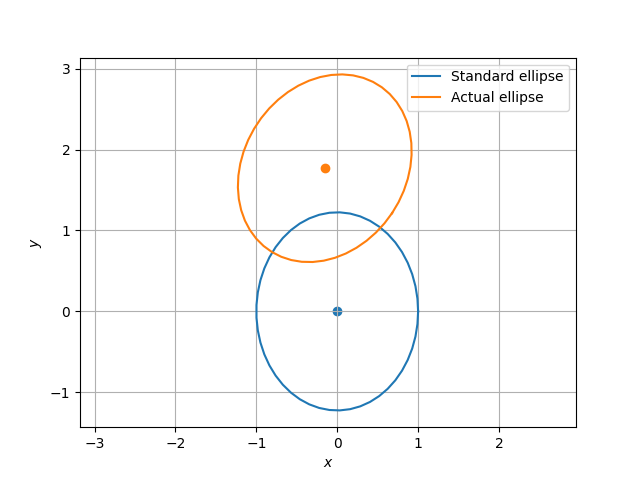
\includegraphics[width=\columnwidth]{./solutions/41/ex/Assignment7.png}

\caption{Ellipse with center \myvec{\frac{2}{13} & \frac{-23}{13}} and having the axes lengths as 1 and $\frac{\sqrt{6}}{2}$}
\label{eq:solutions/41/ex/Fig:Circle}
\end{figure}


\item Trace the curve
\begin{align}
14x^2 - 4xy + 11y^2 - 44x - 58y + 71 =0  \label{eq:solutions/41/ex1/given_curve_eq}
\end{align}

\solution
The general equation of second degree is given by
\begin{align}
ax^2+2bxy+cy^2+2dx+2ey+f=0 \label{eq:solutions/41/ex1/gen_quad_eqn}
\end{align}
and can be expressed as
\begin{align}
\vec{x}^T\vec{V}\vec{x}+2\vec{u}^T\vec{x}+f=0 \label{eq:solutions/41/ex1/conic_quad_eqn}
\end{align}
where
\begin{align}
\vec{V} &= \vec{V}^T = \myvec{a & b \\ b & c}
\\
\vec{u}^T &= \myvec{d & e}
\end{align}

Comparing \eqref{eq:solutions/41/ex1/given_curve_eq} with \eqref{eq:solutions/41/ex1/gen_quad_eqn}, we get
\begin{align}
\vec{V} &= \myvec{14  & -2 \\ -2 & 11}
\\
\vec{u}^T &= \myvec{-22 & -29}
\end{align}
If $\abs{\vec{V}} > 0$, then \eqref{eq:solutions/41/ex1/conic_quad_eqn} is an ellipse. 
\begin{align}
\abs{V} = \mydet{14 & -2 \\ -2 & 11} = 150 > 0 \label{eq:solutions/41/ex1/ellipse_proved_eq}
\end{align}
\eqref{eq:solutions/41/ex1/conic_quad_eqn} can be expressed as
\begin{align}
\label{eq:solutions/41/ex1/conic_simp_temp_nonparab_eq}
\vec{y}^T\vec{D}\vec{y} &=  \vec{u}^T\vec{V}^{-1}\vec{u} -f  &  \abs{V} &\ne 0
\\
\vec{y}^T\vec{D}\vec{y} &=  -\eta\myvec{1 & 0}\vec{y}   & \abs{V} &= 0
\label{eq:solutions/41/ex1/conic_simp_temp_parab_eq}
\end{align}
with center as 
\begin{align}
    \vec{c} &= - \vec{V}^{-1}\vec{u} & \abs{V} &\ne 0
\end{align}
Calculating the center for given curve we get,
\begin{align}
    \vec{c} &= - \frac{1}{\abs{14\times11 - \brak{-2\times-2}}}\myvec{11  & 2 \\ 2 & 14}\myvec{-22 \\ -29} \\
    &= \frac{1}{150}\myvec{300 \\ 450} \\
    &= \myvec{2 \\ 3}
\end{align}
For 
\begin{align} 
\abs{\vec{V}} > 0, \quad \text{or, } \lambda_1 > 0, \lambda_2 > 0 
\end{align} 
\eqref{eq:solutions/41/ex1/conic_simp_temp_nonparab_eq} becomes 
\begin{align} \lambda_1y_1^2 +\lambda_2y_1^2 = 
\vec{u}^T\vec{V}^{-1}\vec{u} -f 
\end{align} 
which is the equation of an ellipse with major and minor axes 
parameters
\begin{align} 
\sqrt{\frac{\lambda_1}{\vec{u}^T\vec{V}^{-1}\vec{u} -f}}, 
\sqrt{\frac{\lambda_2}{\vec{u}^T\vec{V}^{-1}\vec{u} -f}} \label{eq:solutions/41/ex1/axes_eq}
\end{align}
The characteristic equation of $\vec{V}$ is obtained by evaluating the determinant
\begin{align}
\mydet{\lambda \vec{I}-\vec{V}} = \mydet{\lambda -14 & 2 \\ 2 & \lambda -11} &= 0
\\
\implies \lambda^2 - 25\lambda + 150 &= 0
\label{eq:solutions/41/ex1/ellipse_char_eq}
\end{align}
The eigenvalues are the roots of \eqref{eq:solutions/41/ex1/ellipse_char_eq} given by
\begin{align}
\lambda_1 = 15, \lambda_2 = 10
\label{eq:solutions/41/ex1/ellipse_eval_eq}
\end{align}
The eigenvector $\vec{p}$ is defined as
\begin{align}
\vec{V} \vec{p}&= \lambda \vec{p}
\\
\implies \brak{\lambda\vec{I}-\vec{V}}\vec{p} &=0
\end{align}
where $\lambda$ is the eigenvalue.  For $\lambda_1 = 15$,
\begin{align}
\brak{\lambda_1\vec{I}-\vec{V}}
= \myvec{1 & 2 \\ 2 & 4} 
\xleftrightarrow{R_2\leftarrow R_2-2R_1}\myvec{1 & 2 \\0 & 0 }  
\\
\implies \vec{p}_1 = \frac{1}{\sqrt{5}}\myvec{2 \\ -1}
\end{align}
such that $\norm{\vec{p}_1} = 1$.  Similarly, the eigenvector corresponding to $\lambda_2$ can be obtained as
\begin{align}
 \vec{p}_2 = \frac{1}{\sqrt{5}}\myvec{1 \\ 2}
\end{align}
It is easy to verify that 
\begin{align}
\vec{V} &= \vec{P}\vec{D}\vec{P}^{-1}=\vec{P}\vec{D}\vec{P}^T \quad \because \vec{P}^{-1} = \vec{P}^{T} \label{eq:solutions/41/ex1/ellipse_spectrum_eq}
\\
\text{or, } \vec{D} &= \vec{P}^T\vec{V}\vec{P}
\end{align}
where 
\begin{align}
\vec{P} & =\myvec{\vec{p}_1 & \vec{p}_2} = \frac{1}{\sqrt{5}}\myvec{2 & 1\\ -1 & 2} \label{eq:solutions/41/ex1/ellipse_spectrum_P_eq}
\\
 \vec{D} &= \myvec{\lambda_1 & 0 \\ 0 & \lambda_2} =\myvec{15 & 0\\ 0 & 10}
\label{eq:solutions/41/ex1/eq:ellipse_spectrum_D}
\end{align}
Calculating the ellipse parameters using \eqref{eq:solutions/41/ex1/axes_eq}, we get
\begin{align}
\vec{u}^T\vec{V}^{-1}\vec{u} &= \nonumber \\
&= \myvec{-22 -29}\frac{1}{150}\myvec{11 & 2 \\ 2 &1 4 }\myvec{-22 \\ -29} \nonumber \\
&= \frac{1}{150}\myvec{300 & 450}\myvec{22 \\ 29} \nonumber \\
&= 131 \nonumber \\
\vec{u}^T\vec{V}^{-1}\vec{u} -f &= 131 - 71 = 60 \\
\sqrt{\frac{\vec{u}^T\vec{V}^{-1}\vec{u} -f}{\lambda_1}} &= \sqrt{\frac{60}{15}} = 2 \\
\sqrt{\frac{\vec{u}^T\vec{V}^{-1}\vec{u} -f}{\lambda_2}} &= \sqrt{\frac{60}{10}} = \sqrt{6}
\end{align}

Thus, the given curve is found to be an ellipse from \eqref{eq:solutions/41/ex1/ellipse_proved_eq} with center at $\myvec{2 & 3}$ and the major and minor axes lengths are calculated as $\sqrt{6}$, $2$. An ellipse with these parameters along with one having center as origin are plotted as shown.

\begin{figure}[!ht]
\centering
\includegraphics[width=\columnwidth]{./solutions/41/ex1/assignment_6_figure.png}
\caption{Ellipse with center (2 3) and having the axes lengths as $\sqrt{6}$ and 2 along with an ellipse with center as origin}
\label{eq:solutions/41/ex1/Fig:Ellipse}
\end{figure}

\item Trace the following 
\begin{align}
    x^2-3xy+y^2+10x-10y+21=0 \label{eq:solutions/41/ex2/eq 1}
\end{align}
%
\solution
The given quadratic equation can be written in the matrix form as
\begin{align}
    \vec{x}^T\myvec{1&-\frac{3}{2}\\-\frac{3}{2}&1}\vec{x}+2\myvec{5&-5}\vec{x}+21=0\label{eq:solutions/41/ex2/eq:1}
\end{align}
Calculating the parameters,we get
\begin{align}
    \mydet{\vec{V}}=\mydet{1&-\frac{3}{2}\\-\frac{3}{2}&1}=-\frac{5}{4}
\end{align}
Since, $\mydet{\vec{V}} < 0$, therefore the given  equation represents a hyperbola.\par
The characteristic equation of $\vec{V}$ will be
\begin{align}
    \mydet{\vec{V}-\lambda\vec{I}}&=\mydet{1-\lambda&-\frac{3}{2}\\-\frac{3}{2}&1-\lambda}=0\\
    &\implies 4\lambda^2-8\lambda-5 =0 \\
   &\implies\lambda_1=\frac{5}{2},\lambda_2=-\frac{1}{2}\label{eq:solutions/41/ex2/eq 2}
\end{align}
The eigen vector $\vec{p}$ is given by
\begin{align}
 \vec{V}\vec{p}=\lambda\vec{p}
\end{align}
\begin{align}
  \implies{\vec{V}-\lambda\vec{I}} \vec{p}=0 \label{eq:solutions/41/ex2/eq 3} 
\end{align}
For $\lambda_1 = \frac{5}{2} $
\begin{align}
\vec{V}-\lambda\vec{I}= \myvec{1-\frac{5}{2}&-\frac{3}{2}\\-\frac{3}{2}&1-\frac{5}{2}}
    \end{align}
    \begin{align}
 =\myvec{-\frac{3}{2}&-\frac{3}{2}\\-\frac{3}{2}&-\frac{3}{2}}
    \end{align}
    \begin{align}
    \myvec{-\frac{3}{2}&-\frac{3}{2}\\-\frac{3}{2}&-\frac{3}{2}}\xleftrightarrow{R_2=R_2-R_1}\myvec{-\frac{3}{2}&-\frac{3}{2}\\ 0 &0}
\end{align}
 \begin{align}
    \xleftrightarrow{R_1=R_1/-\frac{3}{2}}\myvec{1&1\\ 0 &0}\label{eq:solutions/41/ex2/eq 4}
   \end{align}
Substituting \eqref{eq:solutions/41/ex2/eq 4} in \eqref{eq:solutions/41/ex2/eq 3} we get 
\begin{align}
   \vec{p_1}=\myvec{-1\\1}
\end{align}
Therefore the normalized eigen vector will be
\begin{align}
    \vec{p_1}=\myvec{-\frac{1}{\sqrt{2}}\\\frac{1}{\sqrt{2}}}
\end{align}
For $\lambda_2 = -\frac{1}{2} $
\begin{align}
\vec{V}-\lambda\vec{I}= \myvec{1+\frac{1}{2}&-\frac{3}{2}\\-\frac{3}{2}&1+\frac{1}{2}}
    \end{align}
    \begin{align}
 =\myvec{\frac{3}{2}&-\frac{3}{2}\\-\frac{3}{2}&-\frac{3}{2}}
    \end{align}
    \begin{align}
    \myvec{-\frac{3}{2}&-\frac{3}{2}\\-\frac{3}{2}&-\frac{3}{2}}\xleftrightarrow{R_2=R_2+R_1}\myvec{-\frac{3}{2}&-\frac{3}{2}\\ 0 &0}
\end{align}
 \begin{align}
    \xleftrightarrow{R_1=R_1/\frac{3}{2}}\myvec{1&-1\\ 0 &0}\label{eq:solutions/41/ex2/eq 5}
   \end{align}
Substituting \eqref{eq:solutions/41/ex2/eq 5} in \eqref{eq:solutions/41/ex2/eq 3} we get 
\begin{align}
   \vec{p_2}=\myvec{1\\1}
\end{align}
Therefore the normalized eigen vector will be
\begin{align}
    \vec{p_2}=\myvec{\frac{1}{\sqrt{2}}\\\frac{1}{\sqrt{2}}}
\end{align}
Eigen decomposition\\ 
Since $\vec{V}=\Vec {V}^T$there exists an orthogonal matrix P such that
\begin{align}
    \vec{P}\vec{P}^T=\vec{I}
\end{align}
\begin{align}
    \vec{P}\vec{V}\vec{P}^T=\vec{D}= diag\brak{\lambda_1 \lambda_2}
\end{align}
or equivalently
\begin{align}
    \vec{V}= \vec{P} \vec{D} \vec{P}^T
\end{align}
As
\begin{align}
  \vec{P}=\myvec{p_1&p_2}= \myvec{-\frac{1}{\sqrt{2}}&\frac{1}{\sqrt{2}}\\\frac{1}{\sqrt{2}}& \frac{1}{\sqrt{2}}}\\
   \vec{D}=\myvec{\lambda_1&0\\0&\lambda_2}\\
   \implies 
   \vec{D}=\myvec{\frac{5}{2}&0\\0&-\frac{1}{2}} \label{eq:solutions/41/ex2/eq 6}\\
    \vec{C}=-\vec{V}^{-1}\vec{u}\\
    \implies\vec{C} =\myvec{-\frac{4}{5}&-\frac{6}{5}\\-\frac{6}{5}&-\frac{4}{5}} \myvec{-5\\ 5}\\
   = \myvec{-2\\2}
\end{align}
$\therefore$ Centre C is given by: 
\begin{align}
  \myvec{-2\\2}
%\label{eq:solutions/41/ex2/eq 6}
 \end{align}
 Now Equation \eqref{eq:solutions/41/ex2/eq 1} can be written as
\begin{align}
    \vec{y}^T\vec{D}\vec{y}=\vec{u}^T \vec {V}^{-1}\vec {u}-\vec {f}\\
\end{align}
where y is given by:
\begin{align}
     \vec{y}= \vec{P}^T\brak{\vec{x}-\vec{c}}
\end{align}
So 
\begin{align}
   \vec{y}^T\myvec{\frac{5}{2}&0\\0&-\frac{1}{2}}\vec{y}=-1\\
   \implies \vec{y}^T\myvec{\frac{5}{2}&0\\0&-\frac{1}{2}}\vec{y}+1=0
\end{align}
\begin{figure}[ht!]
	\centering
	\includegraphics[width=\columnwidth]{./solutions/41/ex2/hyberbola.png}
	\caption{Hyperbola plot when origin is shifted}
	\label{eq:solutions/41/ex2/myfig}
\end{figure}


\end{enumerate}


%\section{Exercises}
%

%\section{Triangle Exercises}
%\input{./chapters/tri_geo_exer}
%%
%\section{Quadrilateral Exercises}
%\input{./chapters/quad_geo_exer}
%%
%\section{Circle Exercises}
%\input{./chapters/circ_geo_exer}
%\section{Miscellaneous Exercises}
%\input{./chapters/geo_misc}

\end{document}


